%%% The ``\documentclass'' command has one parameter, based on the kind of
%%% document you are preparing.
%%%
%%% [annual] - Technical paper accepted for presentation at the ACM SIGGRAPH 
%%%   or SIGGRAPH Asia annual conference.
%%% [sponsored] - Short or full-length technical paper accepted for 
%%%   presentation at an event sponsored by ACM SIGGRAPH
%%%   (but not the annual conference Technical Papers program).
%%% [abstract] - A one-page abstract of your accepted content
%%%   (Technical Sketches, Posters, Emerging Technologies, etc.). 
%%%   Content greater than one page in length should use the "[sponsored]"
%%%   parameter.
%%% [preprint] - A preprint version of your final content.
%%% [review] - A technical paper submitted for review. Includes line
%%%   numbers and anonymization of author and affiliation information.

\documentclass[annual]{acmsiggraph}
\usepackage{amsmath}

%%% If you are submitting your paper to one of our annual conferences - the 
%%% ACM SIGGRAPH conference held in North America, or the SIGGRAPH Asia 
%%% conference held in Southeast Asia - there are several commands you should 
%%% consider using in the preparation of your document.

%%% 1. ``\TOGonlineID''
%%% When you submit your paper for review, please use the ``\TOGonlineID''
%%% command to include the online ID value assigned to your paper by the
%%% submission management system. Replace '45678' with the value you were
%%% assigned.

\TOGonlineid{45678}

%%% 2. ``\TOGvolume'' and ``\TOGnumber''
%%% If you are preparing a preprint of your accepted paper, and your paper
%%% will be published in an issue of the ACM ``Transactions on Graphics''
%%% journal, replace the ``0'' values in the commands below with the correct
%%% volume and number values for that issue - you'll get them before your
%%% final paper is due.

\TOGvolume{0}
\TOGnumber{0}

%%% 3. ``TOGarticleDOI''
%%% The ``TOGarticleDOI'' command accepts the DOI information provided to you
%%% during production, and which makes up the URLs which identifies the ACM
%%% article page and direct PDF link in the ACM Digital Library.
%%% Replace ``1111111.2222222'' with the values you are given.

\TOGarticleDOI{1111111.2222222}

%%% 4. ``\TOGprojectURL'', ``\TOGvideoURL'', ``\TOGdataURL'', ``\TOGcodeURL''
%%% If you would like to include links to personal repositories for auxiliary
%%% material related your research contribution, you may use one or more of
%%% these commands to define an appropriate URL. The ``\TOGlinkslist'' command
%%% found just before the first section of your document will add hyperlinked
%%% icons to your document, in addition to hyperlinked icons which point to
%%% the ACM Digital Library article page and the ACM Digital Library-held PDF.

\TOGprojectURL{}
\TOGvideoURL{}
\TOGdataURL{}
\TOGcodeURL{}

%%% Replace ``PAPER TEMPLATE TITLE'' with the title of your paper or abstract.

\title{Adaptive Motion Synthesis by Motion Invariant}

%%% The ``\author{}'' command takes the names and affiliations of each of the
%%% authors of your paper or abstract. The ``\thanks{}'' command takes the
%%% contact information for each author.
%%% For multiple authors, separate each author's information by the ``\and''
%%% command.

\author{Fangde Liu\thanks{e-mail: fliu@bmth.ac.uk}\\Bournemouth University %
\and Richard Southern%
\and Xiaosong Yang%
\and Jianjun Zhang}

%%% The ``pdfauthor'' command accepts the authors of the work,
%%% comma-delimited, and adds this information to the PDF metadata.

\pdfauthor{Fangde Liu,Richard Southern,Xiaosong Yang, Jianjun Zhang}

%%% Keywords that describe your work. The ``\keywordlist'' command will print
%%% them out.

\keywords{Motion Synthesis, Physically Based,CPG, Lie Group}
%\teaser{images/sampleteaser.eps}
%%% The ``\begin{document}'' command is the start of the document.

%%% If you have user-defined macros, you may include them here.

% example of a user-defined macro called ``remark.''
% \newcommand{\remark}[1]{\textcolor{red}{#1}}

\begin{document}

%%% A ``teaser'' image appears under the title and affiliation information,
%%% horizontally centered, and above the two columns of text. This is OPTIONAL.
%%% If you choose to have a ``teaser'' image, it needs to be placed between
%%% ``\begin{document}'' and ``\maketitle.''

\teaser{
   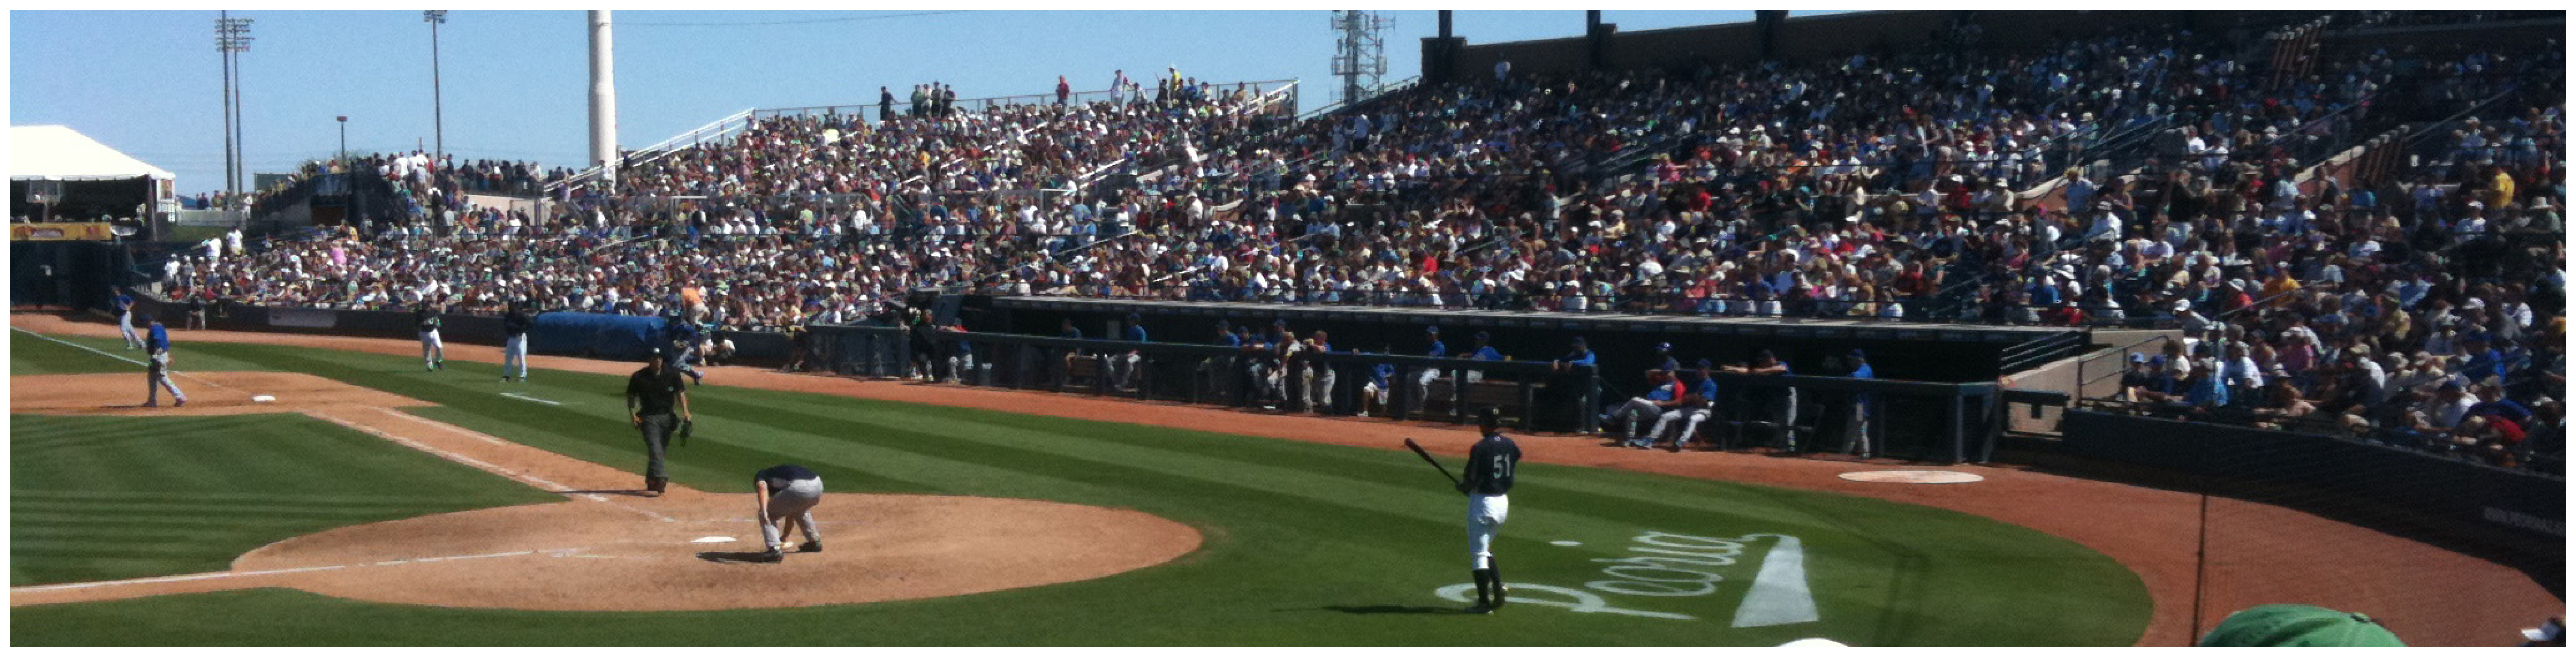
\includegraphics[height=1.5in]{images/sampleteaser}
   \caption{Spring Training 2009, Peoria, AZ.}
}


%%% The ``\maketitle'' command must appear after ``\begin{document}'' and,
%%% if you have one, after the definition of your ``teaser'' image, and
%%% before the first ``\section'' command.

\maketitle

%%% Your paper's abstract goes in its own section.




% Thesis Abstract -----------------------------------------------------


%\begin{abstractslong}    %uncommenting this line, gives a different abstract heading
\begin{abstracts}        %this creates the heading for the abstract page

Generating natural-looking motions for virtual characters is a challenging research topic.
It becomes even harder when generating adaptive motions interacting with the environment. 
Current methods are tedious, cost long computational time and fail to capture natural looking features.

This report proposes an efficient method of generating natural-looking motion based upon a new motor control theory.
The principal idea is motor repertoire is made up of a limited number of elements. Motor control basically connect the basic motion primitives together just like connecting alphabets into sentences.

we propose principle of motor control is not feedback based, they should by model as topology conjugacy.
During motion adaptation, neural system tweaks the basic mechanical system to form an analogous dynamic system that meets constraints and purpose.

When animals adapt their motion, some properties are maintained, which are called motor invariant.
Motion Primitives are identified by the qualitative properties, for which we use the mathematical tools of differential topology.
Tweaking of the motion primitives is model as Symmetry Preserved Transformation, for which we use lie group theory.



Following our idea, we generate adaptive natural looking motion with very little computational costs.
\end{abstracts}
%\end{abstractlongs}


% ----------------------------------------------------------------------


%%% Local Variables: 
%%% mode: latex
%%% TeX-master: "../thesis"
%%% End: 





%%% ACM Computing Review (CR) categories.
%%% See <http://www.acm.org/class/1998/> for details.
%%% The ``\CRcat'' command takes four arguments.

\begin{CRcatlist}
  \CRcat{I.3.7}{Computer Graphics}{Three-Dimensional Graphics and Realism}{Radiosity};
\end{CRcatlist}

%%% The ``\keywordlist'' command prints out the keywords.

\keywordlist

%%% The ``\TOGlinkslist'' command will insert hyperlinked icon(s) to your
%%% paper. This includes, at a minimum, hyperlinked icons to the ACM article
%%% page and the ACM Digital Library-held PDF. If you added URLs to
%%% ``\TOGprojectURL'' or the other, similar commands, they will be added to
%%% the list of icons.
%%% Note: this functionality only works for annual-conference papers.

\TOGlinkslist

%%% The ``\copyrightspace'' command 
%%% Do not remove this command.

\copyrightspace

%%% This is the first section of the body of your paper.

%%% Thesis Introduction --------------------------------------------------
\chapter{INTRODUCTION}
\label{chap:intro}

\graphicspath{{Introduction/IntroductionFigs/EPS/}{Introduction/IntroductionFigs/}}
\nomenclature[z1]{\cms}{Character Motion Synthesis}
\nomenclature[z2]{\cpg}{Central Pattern Generator}
\nomenclature[z3]{\dof}{Degree of Freedom}
\nomenclature[z2]{\moit}{Motor Invariant Theory}

\section{The Challenge}
Character Motion Synthesis (\cms) research aims at generating motion for virtual characters.
It is a topic of significant value in terms of theory and application. 
Besides major applications in the media industry, where both computer games and animation films depend heavily upon character motion for storytelling, 
current research also has applications in user interface design, psychology, sports and medicine.

The challenge of \cms  is not to make characters move, but  to make them lifelike. 
Underlying this challenge is the marvellous human ability of motion perception. 
In real life,people's motion is very similar, yet individuals vary considerably.
From the varieties in motion details, humans can infer mental states, health conditions or the surrounding environment.
%\note{uncanny valley}
Human motion perception has some very peculiar properties.
When wathing a film with computer generated characters, some awkward artefacts are spotted instantly even though they are physically feasible, while many physically impossible motions are accepted as realistic and entertaining. 

%nautral looking

Nowadays in industry, high quality motions are mainly generated manully. 
Very often, characters are complex and contain a large number of joints, making animation tedious work.
To make it worse, reusing motion animation is also difficult and prone to artefacts.
Therefore high level animation tools are badly needed. 

%\note{Do An introduction for physicall based animaiton?}


Real life motions interact extensively with the environment.
Currently, the most important research endeavour is the physics based approach.
Besides  the addition of the dynamic interactive responses, it is  expected that the elimination of  artefacts that violates physics  will make motions more natural looking.
However, this paradigm faces many difficulties:
dynamics of biological systems are much more complex than artificial systems,  attempts to dynamically simulate biological system face prohibitive  computational costs and modelling difficulties.
In fact, such problems have already been identified by biological researchers.







Motor Control and Motion Perception are close related.
Difficulties in \cms reflect the inferiority of artificial control method.
The peculiarity of motion perception and control suggests  biological systems may adopt a different principle.
To generate natural looking motion, it is worthwhile to synthesize motion following the biological motor control principle. 
This thesis is founded on new ideas from biological research.

 

\section{Agile Animals}
%\note{Underlying these problems} is our misunderstanding of animal motions.
Although animals have fascinated us for thousands of years, we still do not fully understand how they move.
Animals are very different from artificial machines and such comparisons may reflect the  biological motor control principle.
%some basic questions of motor control and motion perception remain open. 
%And answers to such questions become even more valuable nowadays. 
%Advance in this topic will greatly influence the biology, robotic engineering even intelligent research.
%\note{The difference between biological motor system}

%The paradoxes is even human are good at motor control and motion perception; human still don’t have an idea of how we move and how we perceive motion.
%Before going into details into the research ideas, we first review some puzzles troubles the foundation of CMS. 
\begin{itemize}
\HiItem {Degrees of freedom ({\dof}s)}.
From a mechanical perspective, animals have many more {\dof}s than their artificial counterparts.
An artificial ship can be approximated by a simple rigid body; whereas the flexible vertebrae of a finsih is made up of tens of {\dof}s.


In principle, the extra {\dof}s allows for more variations in adapting the environment. 
However, for the control system, too many extra {\dof}s are a disaster because of the computational burden. 
For a human to take one step,  the neural system controls more than $600$ muscles.
Even with nowadays computer, solving the dynamics directly would spend thousands of hours.

 
\HiItem {Versatility}
Most artificial machines are designed with a single purpose,while animals are capable  of unlimited tasks.
Many biological functions which are often neglected by \cms research, such as feeding, breeding, language and vision, depend on motor control. 
Besides walking, swimming and many other styles of locomotion, we utilize many tools, such as cars, skates, bicycles and tennis rackets.

Following traditional control methods, it seems that unlimited resources need to be  allocated for motor control, while biological research shows motor control requires very few mental resources.

\HiItem{Performance}
Although the problem of biological motor control is more complex, the resulting performance surpasses artificial machines in many aspects.
Natural motions are more
\begin{enumerate} 

\HiItem{Robust:}
A human can maintain walking stability on rough terrains which would be inaccessible for vehicles.

\HiItem{Manoeuvrability and speed:}
Typical modern aeroplanes  travel at a maximum of $32\: body\: length/sec$ and yaw at $720\: deg/sec$.
While pigeons may travel at $75 \:body\: length / sec$, yaw at about  $5000 \: deg/sec$.

\HiItem{Energy Efficiency:}
The energy consumed by a human walking is only $5\%$ of that for the world famous humanoid ASIMO.
\end{enumerate}

\end{itemize}



%For computer animation research, the key principle is we should know the things we animate.
%Natural motion system has many valuable properties which are not captured by current motion synthesis methods.
%\begin{itemize} 
% \HiItem{robust}
%Natural motions are adaptive to the changes in the environment or body conditions. 
%A common example is human locomotion. 
%Walking on different terrains will exhibit different gait while the balance is maintained. 
%
%\HiItem{speedy}
%Some motions of animals are very fast, honey birds may vibrate their wings in kHz.
%The astonishment is to the speed of motion, more puzzling is that the neural system can solve the complex motion control problem in such a short time. 
%When an animal avoids obstacles at very high running speed, 
%it must continue its running, make a turning and keep balance at the same time. 
%It seems easy for the neural system to plan complicate motions.
%\HiItem{Energy Efficient}
%Natural Motions are energy efficient.
%In theory, this idea is supported by Darwin's Theory of Evolution.
%But animals spent far less energy than our expectation.
%An example is that the energy consumed by human walking is only 5\% of that for a robot of the same scale.
%\end{itemize}

\section{Motor Invariant Theory}
\subsection{Utilizing Natural Dynamics}
Biological Motor Control has achieved a delicate balance of robustness, controllability and energy efficiency.
The real-time performance may further suggest that the biological method  is simple and requires little computational load.
These are the dreaming properties for \cms research and  the explanation that how biological system achieve this  forms the genesis of this thesis.



Interactions between the body and environment pose  complex dynamic problems for motor control.
In most \cms research studies, such natural dynamics are treated as noises or perturbations to motion planning, and the  effects  of natural dynamics are cancelled by control effort.
However from an evolutionary perspective, the mechanical structures are a product of natural selection which has evolved alongside with the environment for millions of years. 
These structures are an advantages rather than a handicap. 
Without the need to consider stability, energy efficiency and real-time constraints, motor control can be easily achieved if the motion is totally governed by natural dynamics and requires no control effort.
A new idea is that motor control is based on natural dynamics.
The neural system plays a minor role in planning; it simply utilizes natural dynamic properties.

Motor Invariant Theory (\moit)  proposes  how to utilize the natural dynamics in a systematic manner.








\subsection{Motor Invariant Theory}
%In this thesis, we propose different idea towards motor control and motion synthesis.
%In this research, we propose a different motion synthesis method based on a different motor control theory.
%
%An insightful discovery is that motor control can be “easy”.
%For some situation, some tasks mainly explore the properties of the body and environment and can be achieved with little control effort.
%In nature, we don’t finish difficult motion tasks, we select many easy motion tasks that we are good at, connect or modify them for our special purpose.
%
%The “easy” tasks are called motion primitives; they are the basic elements of our motor ability. 
%When we modify the motion primitives, some valuable properties of motion primitives are kept unchanged, and the maintained properties are called motor invariants.
%
%The inspiration of our idea comes from related biological research, which covers biomechanics and neural science.





This thesis proposes a new idea for the underlying reason for superiority of biological motor control.
The insight is that in the process of motion adaption, some valuable properties of natural dynamics are kept invariant.
The conjecture is that:  instead of detecting and cancelation all kinds of perturbations, biological motor control relies on the invariance of natural dynamic properties for motion success.
This is \emph{Motor Invariant Theory(\moit)}.


\moit incorporates the motion primitive conjecture.
In dynamics, invariant properties are stable properties. 
From a dynamic perspective, not all the motions generated by natural dynamics are stable, only the stable ones are utilized and treated as the templates.
In dynamics, invariant properties are stable properties.
From a dynamic perspective, not all the motions generated by natural dynamics are stable, only a few are stable, which can be utilized motion templates and become motion primitives.
The remaining question is how the motor control system utilizes the templates to synthesize motion.

The \moit propose that when facing a new situation, human don't solve motor control from ground up,
motor control system utilizes successful experience in similar situations.
In dynamics, adapted motions are qualitative the same with the motion primitives or templates.
In dynamics, adapted motions are qualitative the same with the motion primitives or templates, and there is a one-one mapping relationship between the adapted motion and the motion primitive.
This similarity in dynamics is topological conjugacy. 

In dynamic \cms research, a motion is represented by  a curve  $x(t)$ parameterized by $t$.
$x(t)$ is the solution to the equation (Equation ~\ref{eq:BodyEnvDym}) that describes the body and environment dynamics.
\begin{equation}
\dot{x}=F(x)
\label{eq:BodyEnvDym}
\end{equation}


To illustrate adaptation, we define a transformation $T$ that acts on the space of $x$.
\[
\tilde{x}=T(x)
\]

In this way, each equation can be described in two coordinate systems: one by $x$ and one by $\tilde{x}$.
As an example, Equation ~\ref{eq:EQtransform} is describes the same dynamics as  Equation ~\ref{eq:tranformedEQ} in a different coordinate system.
then we can obtain two equations in  the transformed state $\tilde{x}$ ( )and original state $x$(Equation ~\ref{eq:EQtransform}).

\begin{equation}
\dot{\tilde{x}}=F(\tilde{x})
\label{eq:tranformedEQ}
\end{equation}

\begin{equation}
\dot{x}=\tilde{F}(x)
\label{eq:EQtransform}
\end{equation}

Since such two equations describe the same motion in different coordinate systems, the solution to one equation can be achieved by transforming the solution to the other equation.
Supposing $x'(t)$ is the solution to Equation~\ref{eq:EQtransform} and $\tilde{x}(t)$ is the solution to the Equation~\ref{eq:tranformedEQ}, then we have
\[
x'(t)=T^{-1}(\tilde{x}(t))
\]
Equation~\ref{eq:tranformedEQ} and Equation~\ref{eq:BodyEnvDym} are the same, thus: 
\[
\tilde{x}(t)=x(t)
\]
Then we have
\[
x'(t)=T^{-1}(x(t))
\]

By transformation, we obtained a new motion $x'(t)$ from $x(t)$.





%if we substitue x=f(x,t) into (1).
%we can express equation (2) interm of (x,t,x)
%\dot(x)=F'(x).
%then the solution of the equation becomes 
%x2(t)=(x)t=f-1(xt)
%
%
The  transformation method has many advantages: it is much less computational expensive and keeps many important properties untouched.
For example, if the original dynamics is stable, then the transformed dynamics is also stable. 
%
If there exists continuous one-one mapping between the two dynamic equations, then the two are \emph{topological conjugate}.
This relationship is presented by $F \simeq \tilde{F}$.
$F$ and $\tilde{F}$ are called \emph{analogous systems},, which share the same topology structure.
The existence of one-one mapping is the necessary and sufficient condition for topological conjugate, thus there are two basic approaches for motion adaption.
Transformation can be specified explicitly or implicitly by maintaining the topology.



If the perturbation does not violate the topology, the corresponding one-one mapping will modify the motion without changing it qualitatively.
In dynamics,the topology preserving ability is an intrinsic property of many dynamic systems:
\emph{structural stability}.
One strategy of motor control is to enhance the structural stability. 
With this approach, the qualitative property is preserved and there exists a one-one mapping relationship, but finding out details of motion will be difficult or computational expensive.
Therefore this approach is qualitative.

In \moit,this approach models the involuntary motion adaptation which is low level function of neural control system.
The topological structure is one important property should be kept invariant, thus become a motor invariant in \moit: the \emph{Global Motor Invariant}.






Also if the transformation is known, then the two systems must be topological equivalent.
This method  modifies motion with precision and \moit applies this idea for high level voluntary motor control.
In many situations, to achieve desired transform $T$, control effort needs to be applied.
For this method, choosing a proper transformation $T$ is the most challenging  question.

In \moit, selection of $T$ is based on two principles.
\begin{itemize}
\item
Parameters of transformation $T$ should be easy to detect and formulated, which meets the biological sensing and computational constraints. 

\item 
The transformation $T$ should be energy efficient.
For differential dynamic system, some transformation explores the natural dynamics and requires little or no energy input.
\end{itemize}
Some quantitative properties will be unchanged during transformation, which are called \emph{Local Motor Invariant}






%the stability of the orignal system is known.
%if possible, we always try to tranform the stable motion.
%To this end motor control are applied to execute the transformation
%
%
%
%these two ideas have pros and cons.
%The first method maintail the qualitative properties, but details of motion can not be controlled precisely.
%if the second method is applied, given the transformation, the resulting motion can be know, while but to carried out such transformation, controll effort may needed.
%
%




Although new mathematical language seems obscure at first glimpse, the properties that the mathematical language describes are universal in physical world, with or without life.
The underlying idea is intuitive and can be explained well through commonly observed phenomena.



\subsection{The Floating Ship: An example of Stability}
The floating ship  example shows the idea of structural stability and topological conjugacy.
In real life, ships floating on the wave are typically taller than they are wide,as shown in Figure~\ref{fig:ShipFloating}.
An interesting  question is how the ship maintains its posture.

Through analysing the topology and structural stability, we see that it is trivial to maintain posture.
This conclusion applies to different ships since their dynamics are qualitative the same, or topological conjugate.


\subsubsection*{Dynamics}

\begin{figure}[!htbp]
  \begin{center}
    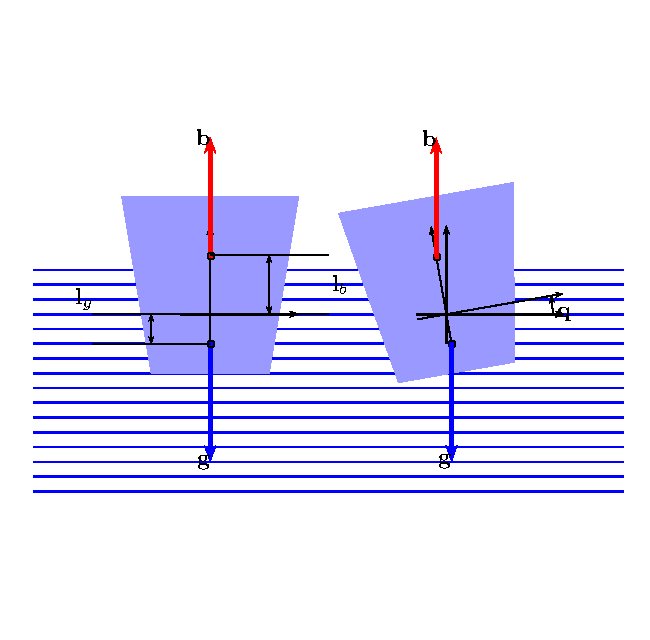
\includegraphics{ShipExample}
    \caption{The Floating Ship Example}
    \label{fig:ShipFloating}
  \end{center}
\end{figure}

The sway motion of the ship shown in Figure ~\ref{fig:ShipFloating} can be described by Equation~\ref{eq:shipflow}
\begin{equation}
\label{eq:shipflow}
J\ddot{q}+d\dot{q}=\tau(q)_{g}+\tau(q)_{b}+\tau_{u}
\end{equation}


where $q$ is the swaying angle.
$J$ is the inertia,  
$d$ is the damping coefficient,
and $\tau_{g}$,$\tau_{b}$,$\tau_{u}$ are the corresponding the torques of gravity, buoyancy and external control.

When a ship is on the sea, the motion is governed by the two forces, the buoyancy $b$ and gravity $g$.
When $\tau_{u}=0$,  the dynamics is becomes governed by its natural property.
Such a system is \emph{autonomous}.

To make it consistent with discussions in following chapters, Equation~\ref{eq:shipflow} is reformulated.
Defining the \emph{state} variable $\state=[q,\qd]$, then Equation~\ref{eq:shipflow} becomes
\[
\dot{\state}=F_{J,d}(\state)+Du
\]

where 
$F$ is a function of $\state$, the subscripts~$J$ and~$d$ are \emph{system parameters},
$D$ is a matrix, which describes how the control effort is applied,
and $u$ is \emph{control input}, for this example $u$ is $\tau_{u}$



\subsubsection*{Equilibrium Postures}
A ship will only rest when $\tau_{g}+\tau_{b}+\tau_{u}=0$, which are called \emph{Equilibrium} Postures.
The only two possible ones are show in Figure ~\ref{fig:ShipEqulibriumStable} and Figure~\ref{fig:ShipEqulibriumUnstable}.
\begin{figure}[!htbp]
  \begin{center}
     \includegraphics{leftPos}
    \caption{The Stable Equilibrium Posture}
    \label{fig:ShipEqulibriumStable}
  \end{center}
\end{figure}

\begin{figure}[!htbp]
  \begin{center}
     \includegraphics{rightPos}
    \caption{The Unstable Equilibrium Posture}
    \label{fig:ShipEqulibriumUnstable}
  \end{center}
\end{figure}



The two postures are different, illustrated with the \emph{phase plot}.
On the phase plot, the horizontal axis represents  $q$; and the vertical axis represents velocity $\qd$. 
The motion of the ship is shown as a curve on the phase plot, which is called \emph{flow}.

The posture in Figure ~\ref{fig:ShipEqulibriumStable} is \emph{attractive} or \emph{stable},
for if a small perturbation moves the ship away from the left posture, it will return to the equilibrium posture automatically as shown in Figure~\ref{fig:StablePosture}.
\begin{figure}[!htbp]
  \begin{center}
      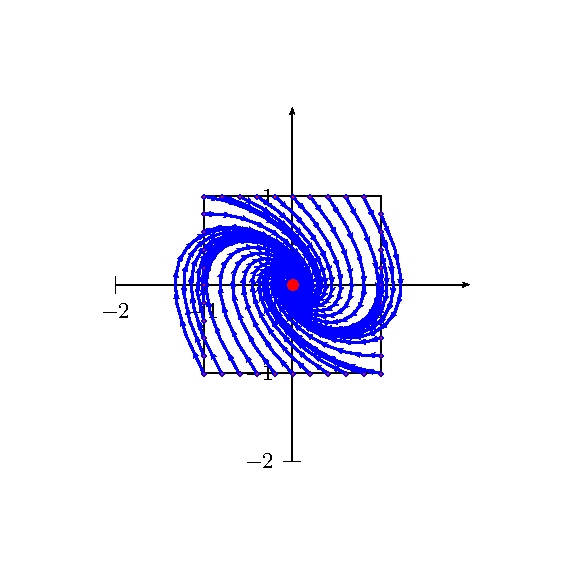
\includegraphics{stablePosition}
    \caption{Phase Plot of the Stable Posture}
    \label{fig:StablePosture}
  \end{center}
\end{figure}


Whereas the  posture in Figure~\ref{fig:ShipEqulibriumUnstable} is \emph{repelling} or \emph{unstable}, if being moved away from the equilibrium posture, the ship will move away further, as shown in Figure~\ref{fig:unStablePosture}.

\begin{figure}[!htbp]
  \begin{center}
      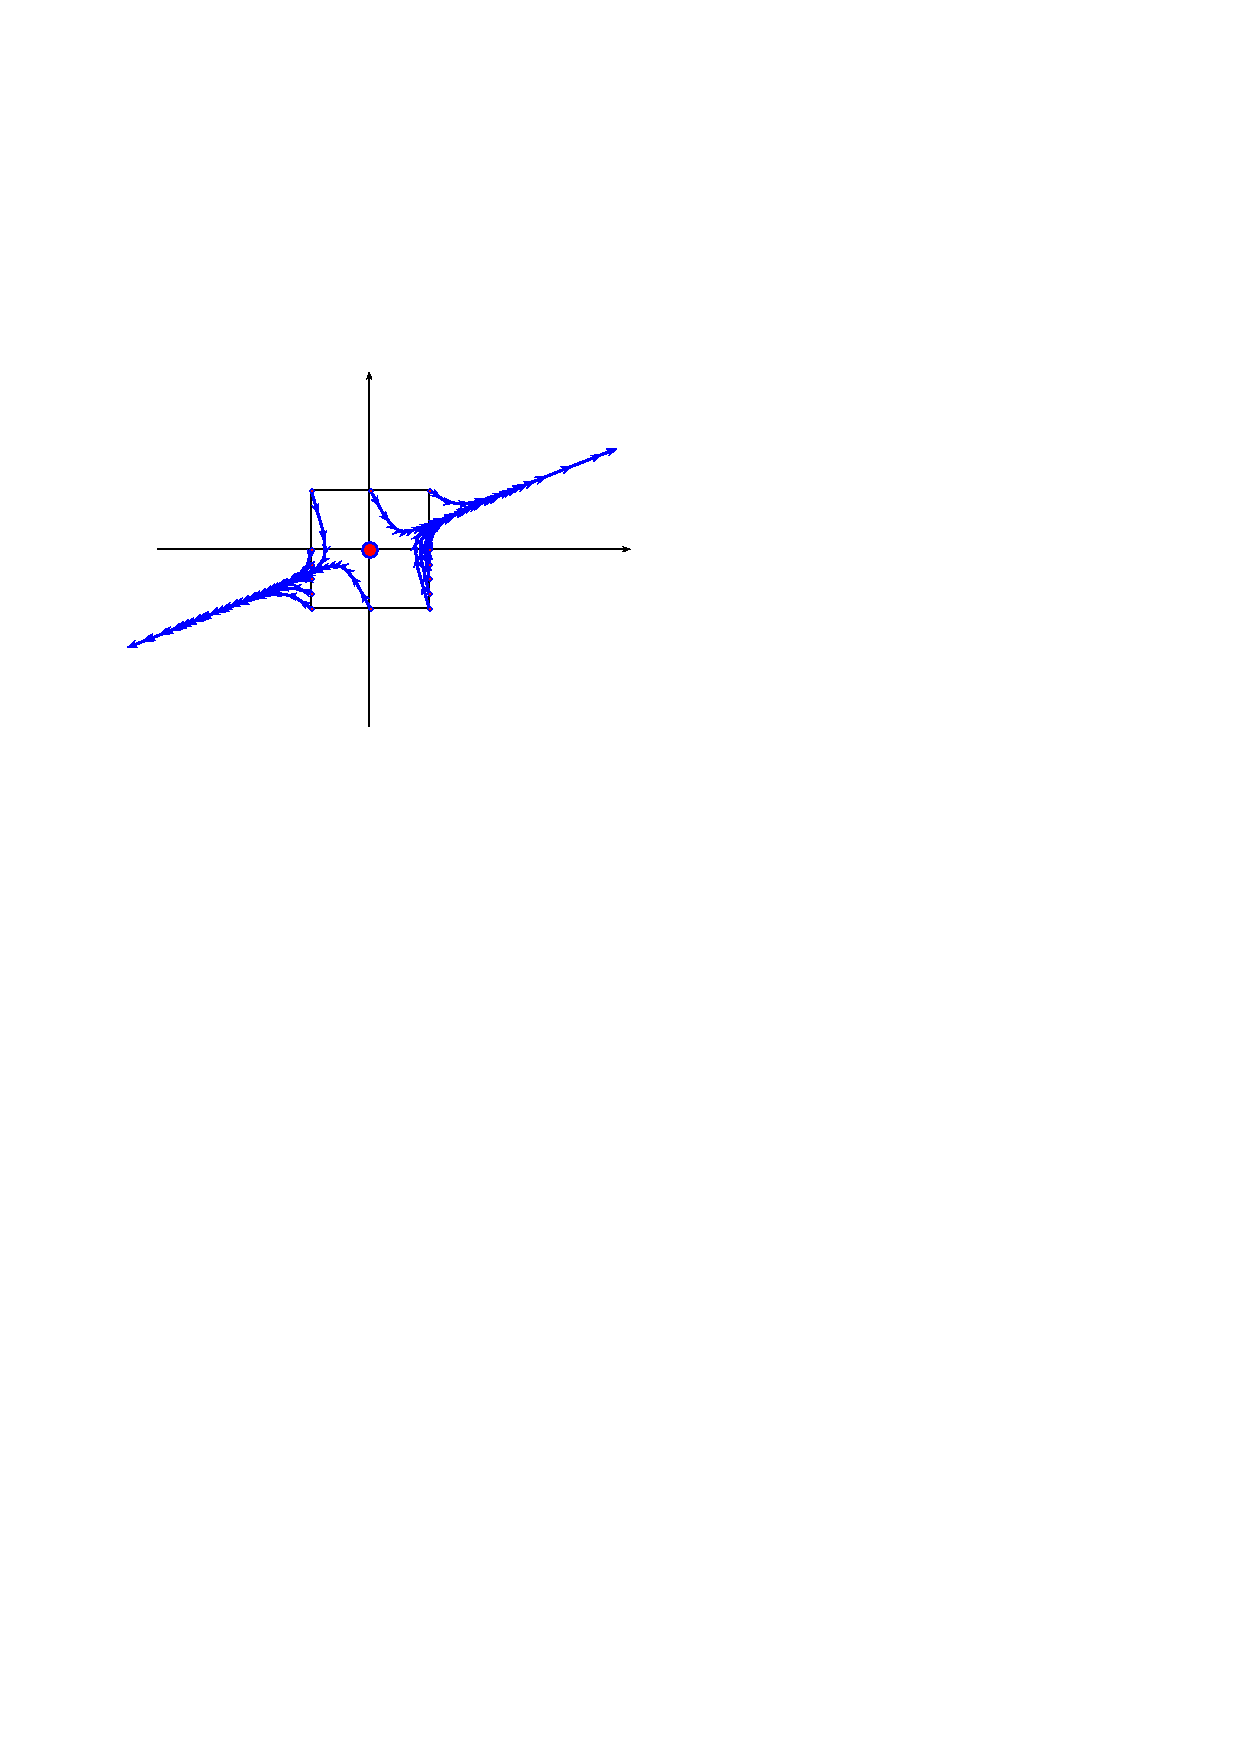
\includegraphics{unstablePosition}
    \caption{Phase Plot of the Unstable Posture}
    \label{fig:unStablePosture}
  \end{center}
\end{figure}


\subsubsection*{Trivial Task}
All the flows form the \emph{phase portrait} of the dynamic system. 
The discovery is that all the flows start from the repelling posture and ends at the attractive posture.
Several example curves are show in Figure ~\ref{fig:globalflow}.
This means no matter what the current posture is, the ship will return to the normal stable posture automatically.

This is an intrinsic property of the natural dynamics, and thanks to this, balancing is a trivial task which requires no control effort. 
This property is determined by the qualitative structure design criteria, makeing the centre of buoyancy  above the centre of gravity.

\begin{figure}[!htbp]
  \begin{center}
   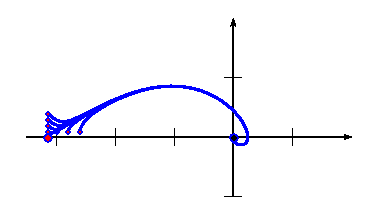
\includegraphics[width=0.7\textwidth]{ShipGlobalFlow}
   \caption{Global Properties of the Flows: All the curves start from the repelling posture(Red) and end at the attractive one(Blue)}
   \label{fig:globalflow}
  \end{center}
\end{figure}

 



\subsubsection*{Generalization of the Ship Example} 
This conclusion is independent of the shape, size, weight or material of the ship. 
In general cases, the same wave perturbation will result in different sway motions for different ships.
Howerver, as long as the qualitative structure design criteria is maintained, balancing remains ``easy''.
On phase portraits,  all the ships share following properties. 
\begin{itemize}
\item one repelling point 
\item one attractive point 
\item all flows start from repelling point and end at the  attractive point. 
\end{itemize}

In mathematical terms, all the phase portraits share the same topology structure of Figure~\ref{fig:topologyStructure}.

This phenomenon illustrates the principle idea of motion adaptation in \moit.
When the variations among individuals or situations result in motion variation, the qualitative dynamics or topological structure of the dynamic system remains invariant.

\begin{figure}[!htbp]
  \begin{center}
   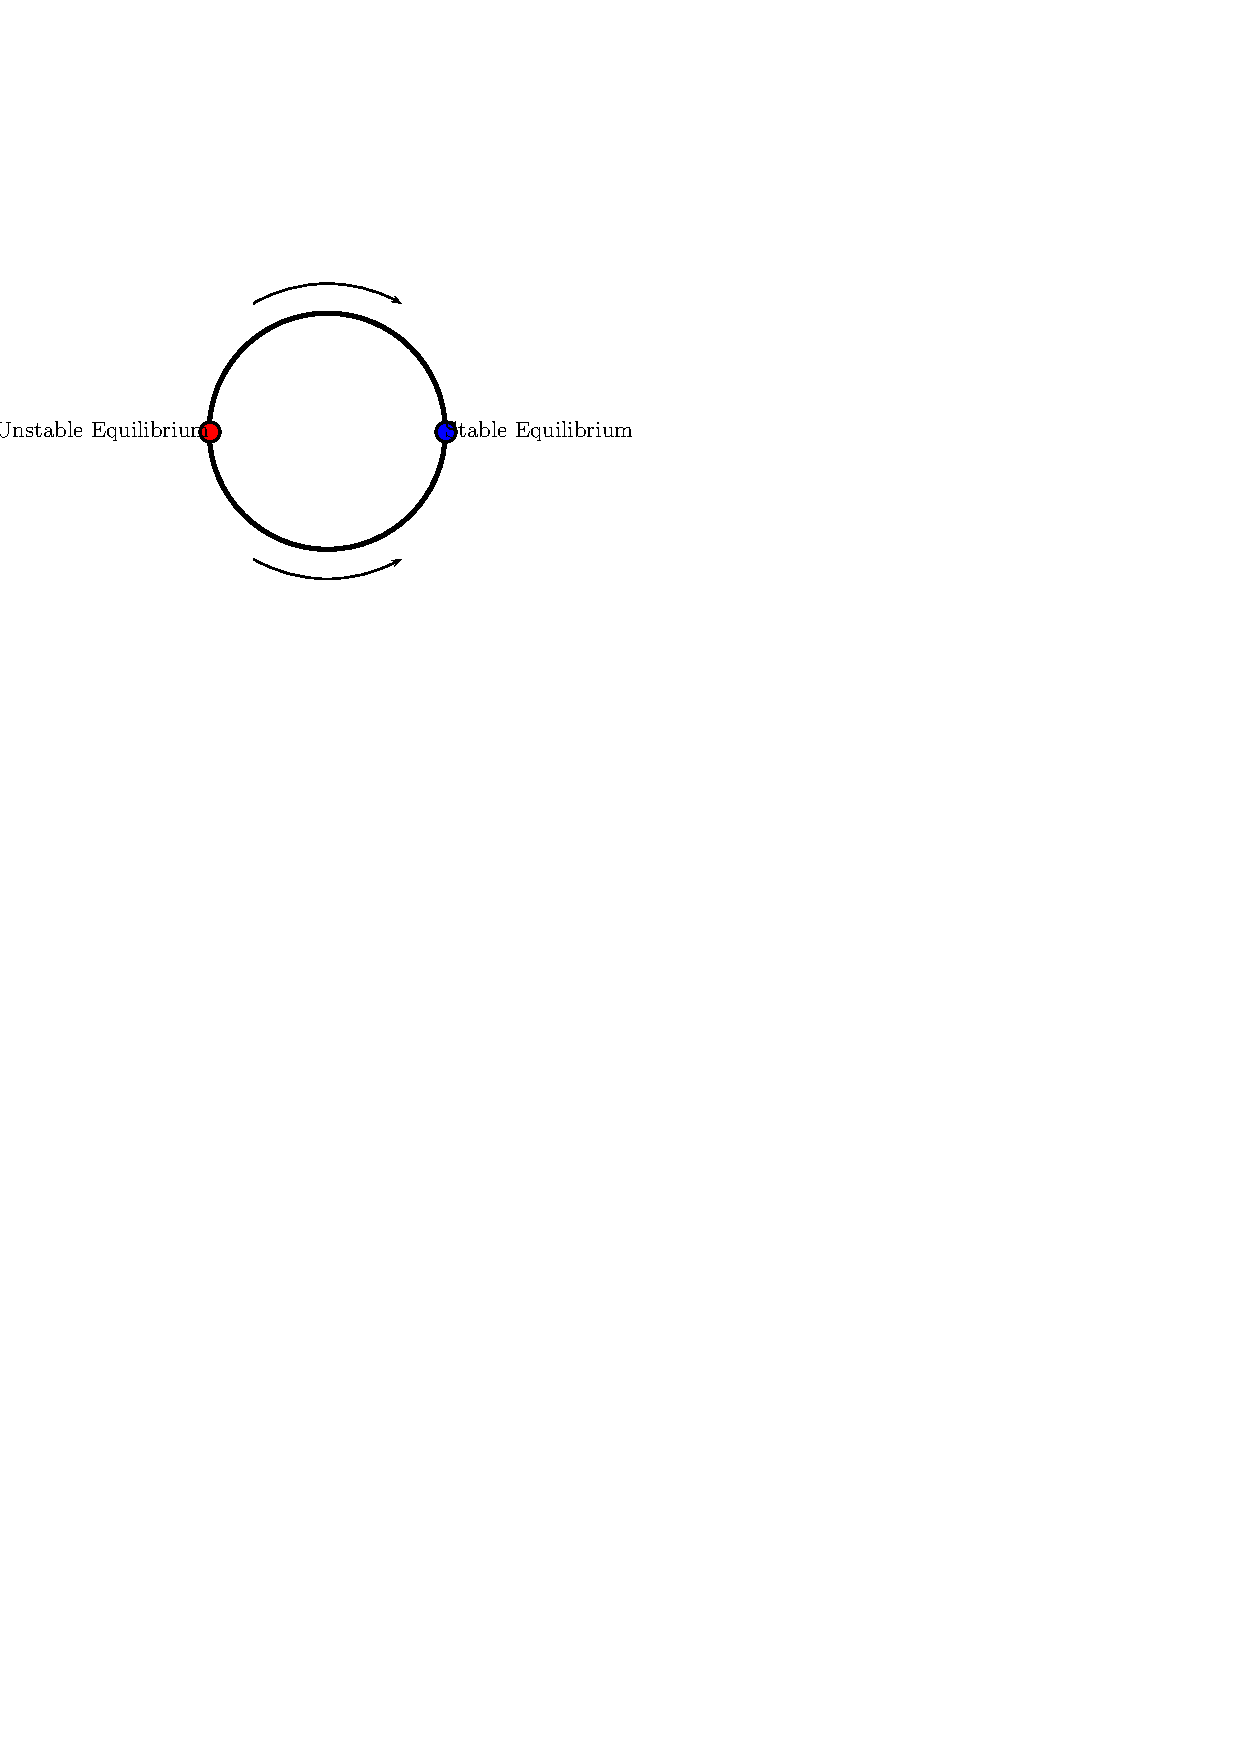
\includegraphics{topologyStructure}
   \caption{the topology  the phase portraits of ship dynamic}
   \label{fig:topologyStructure}
  \end{center}
\end{figure}




\subsection{The Mass Spring System:  Symmetry Transformation}
Despite the complexity of body structure, biological motor control is fast and accurate.
Such quantitative properties pose another puzzle in motor control research, as solving the complex dynamics directly would require prohibitive long computational time and excessive mental resources.

\moit proposes a new method to achieve the  speed and accuracy of motor control.
An efficient control strategy is based on the idea of transformation.
Without solving the dynamics, new motions are achieved through transforming template motions.
To keep the motion natural looking, control system chooses the transformation directions that are energy efficient, or in another term, allowed by the natural dynamics.


Such ideas can be illustrated by the following mass spring example, shown in Figure~\ref{fig:massspring}.
The mass spring system is selected for it captures some important properties of biological dynamics.
The compliant actuators of muscles work like springs, and rigid bones are modelled as mass.


\begin{figure}[!htbp]
  \begin{center}
    \includegraphics[width=0.7\textwidth]{MassSpring}
    \caption{the mass spring system}
    \label{fig:massspring}
  \end{center}
\end{figure}

\subsubsection*{Dynamics}
The canonical equation of mass spring system is
\begin{equation}
\label{eq:mass-spring}
\ddot{q}+q=0.
\end{equation}
where $q$ is the offset distance.

By defining the \emph{state variable}, $\state=[q,\qd]$, Equation~\ref{eq:mass-spring} can also be reformulated in the form as
\[
\dot{\state}=F(\state)
\]

 Figure~\ref{fig:massSpringPhasePlot} shows two flows passing through different states $x$ and $x'$ on the phase plot.


\begin{figure}[!htbp]
  \begin{center}
     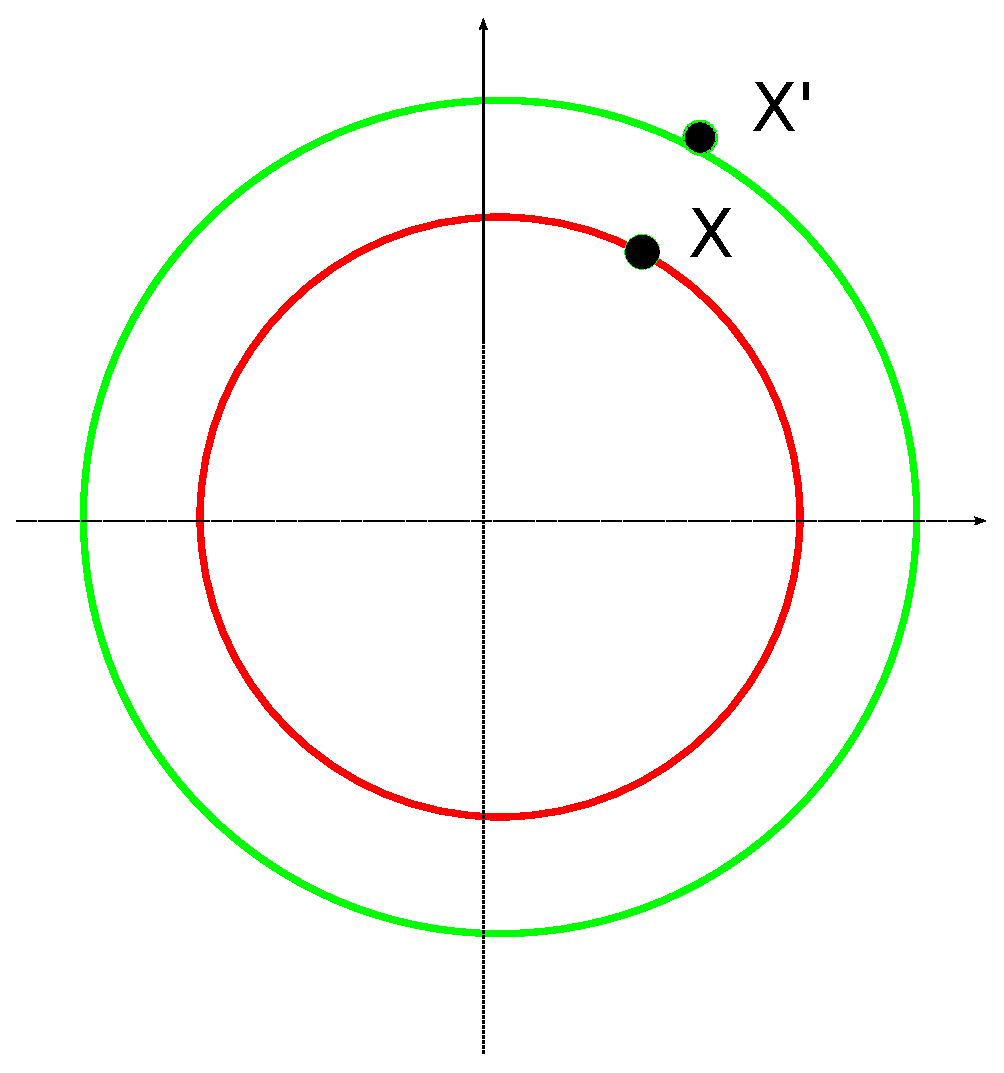
\includegraphics[width=0.5\textwidth]{MassSpringPhasePlot}
    \caption{Mass Spring Phase Plot:two motion curves are shown.The red one and the green pass through different states ($\state$ and $\state'$}
    \label{fig:massSpringPhasePlot}  
  \end{center}
\end{figure}

\subsubsection*{Symmetry and Transformation}
%It is highly unlikely animals can solve Equation~\ref{eq:mass-spring}.

The mass spring system has some ``symmetrical properties''.
Different flows share the same circle ``Shape''.
Without sovling the Equation~\ref{eq:mass-spring}, neew flows(solid ones) can be obtained by scaling the original(red) flow.

From a mechanical viewpoint, this is because the flows of mass spring system are energy preserving.
We can define the energy function
\[
E=\frac{1}{2}(m\qd^2+kq^2)
\]
where $k$ is the stiffness, $m$ is the mass.
When $m=1,k=1$, since $E$ is a constant, we can take $E=c$,
and obtain $q^2+\qd^2=2c$, which is the implicit function of a circle.

Therefore, given the template flows that pass through  $\state$, for the state $\state'$, by checking the energy, the scale transformation from red to green can be worked out.
In this manner, we botained the future motion after $\state'$, without sovling the dynamics.


\subsubsection*{Dynamic Perception and Local Motor Invariant}

The idea ``transformation and symmetry'' may shed light on dynamic perception. 
It is highly unlikely animals can solve Equation~\ref{eq:mass-spring} to understand mass spring system.
As an alternative, the dynamics can be encoded in a different manner: a motion template and the symmetry property. 
If so, observed motions can be validated by being checked against motion templates in our memory.

To make it better, it is even unnecessary to working out the transformation, it is enough just to check some property invariant under transformation.
For the mass spring system example, we can check the “shape” of the flow, or from a mechanical perspective, check the energy preserving property.

 
The invariant properties like energy preserving or shape can be quantitative measured, they are invariant only when system flows move in a specific direction, thus are called  \emph{Local Motor Invariant}. 


\section{Contribution}

Compared with current \cms methods, the new approach has several advantages:
\begin{enumerate}
\HiItem {More Types of Adaptation}
Most dynamic methods only focus on generating responsive motion to dynamic perturbation.
Adaptations across different characters are solved with a different method and treated as a independent research topic(motion re-targeting).
\moit unifies different  adaptations in one theory.
The mathematical idea of topology conjugacy  incorporates both motion re-targeting and  perturbation responses  in an unified framework.
Thus \moit can generate more types of adaptation.
\HiItem {Better Usability}.
For many \cms methods, each \dof ~is controlled independently.
When modifying motions, animator has to modify each \dof, which is tedious work.

In \moit, adaptation is achieved by applying transformation.
Each transformation can be parameterized by one parameter. 
By specify only one parameter for the transformation, control inputs of all {\dof}s are modified automatically, which is more easy to use.

\HiItem {No Reference Motion Needed}
\moit relies on the dynamics of body and environment.
Motion Capture Data is not needed as reference input.
In situations, this method can generate new motion that can not be captured.


\HiItem {Computationally Efficient} 
This motion synthesis approach requires little computation time and memory, it suits real-time applications.
\HiItem {Dynamic Motion Transition}
Dynamic motion transition is developed upon solid theory foundation.

\end{enumerate}

Because of its biological foundation,
algorithms and simulation results of \moit  might shed light into biology research.
Some conclusion and control techniques can be treated as candidate theory that needs further verification.

\begin{enumerate}
\item 
Motion Primitive is an old idea in biological research, but there is no agreement on the definition and underlying reason.
Biological research has tried to identify motion primitive by exploring the neural anatomy, EMG signal or muscle activation pattern.

\moit  explains the motion primitive from dynamic viewpoint.
This theory is more complete.
Besides identification, it also answers why certain motions are primitives and others are not,
how many motion primitives we have,  and where they come from.

\item One supporting theory of motion primitive is the muscle synergy:
Generating motion by actuating muscles, muscles are not controlled independently but worked in group. 
Many research in synergy by empirical methods. 

In \moit, when control is applied to ensure transformation, actuators are controlled in an ``synergy manner''.
\moit provides a candidate  ``synergy'' method for muscle control.

\item For the neural structure \emph{Central Pattern Generator}(\cpg) , their roles in motor control are well agreed.
While detail strategy for adjust \cpg parameters according to motor purpose is still lacking.
The \moit provides an theory for modifying the \cpg parameters with mathematical rigidity.


\item  Motion and dynamic perception mechanism of neural system is still unclear.
The motor invariant theory proposes a computationally efficient mathematical machinery.
\end{enumerate}







\section{Organization of the Thesis}

This thesis is organized as follows.
 
In Chapter~\ref{chap:background}, previous research on motion synthesis and biological motor control are discussed, which are the motivation and justification of \moit.
 
In Chapter~\ref{chap:gi}, \emph{Qualitative Dynamicss} is introduced to explain motion primitives. 
Biological based  methods for maintaining the global motor invariant are developed.

Chapter~\ref{chap:li} focuses on the idea of Local Motor Invariant and Symmetry.
Lie Group theory is  introduced  to analyse the symmetry properties in motion dynamics.
Symmetry Controllers are developed for adaptation motions.
 


Chapter~\ref{chap:msf} discusses the combination problems.
For each motion primitive,  strategies are developed to preserve global and local motor invariant simultaneously.
Motion primitive transition is discussed and methods for combining motion elements into more complex motion is discussed.
As an animation system, the software architecture and work flow are discussed at the end.

Chapter~\ref{chap:gi},~\ref{chap:li},~\ref{chap:msf} lay the theoretical foundation of \moit.
Following chapters focus on application in \cms.



Chapter~\ref{chap:walk} focuses the tweaking of one primitive.
Bipedal walking is chosen, which is one of the most challenging problem for current \cms research.
Motor Invariant Theory introduces a method to boost the stability and generate adaptive gaits.


In Chapter~\ref{chap:stance}, combinations of motion primitives are discussed.
A new balancing motion primitive is developed. 
Transitional motions are generated for stance to walk and walk to stance transitions.

In Chapter~\ref{chap:highdor}, extensions of motor invariant theory to more complex characters are discussed.
Three strategies are developed to simplify the problem for different situations.

This thesis ended with Chapter~\ref{chap:con}. 
After discussion of new finding of this research, some new questions and ideas for graphics and neural science are proposed for further research .





%%% ----------------------------------------------------------------------


%%% Local Variables: 
%%% mode: latex
%%% TeX-master: "../thesis"
%%% End: 


\chapter{BACKGROUND}
\label{chap:background}

\nomenclature[z3]{\pd}{Proportional Derivative}
\nomenclature[z4]{\lc}{Limit Cycle}
\nomenclature[z5]{\cpg}{Central Pattern Generator}
\nomenclature[z6]{\eph}{Equilibrium Point Hypothesis}
\nomenclature[z7]{\umh}{Uncontrolled Manifold Hypothesis}
Underneath different \cms methods, are different ideas of motor control.
Current \cms research follows the control idea for artificial system.
There is a clear speration of planning and execution in traditional controller design.
In the \cms research, body are treated as mechanical apparatus, which execute the motion planned by the neural system.

Motor Invariant Theory is based on the intergrative theory of motor control\citep{dickinson2000animals}.
In the integrative view, there is no a clear seperation between planning and execution,  motor control can only be understood as a whole.

In this chapter, limitation of current \cms research are discussed first for they are the motivation of this research.
New theory is developed because such limitations can not be overcome within the current framework.

Later some biological research are discussed later, for they are the foundation upon which motor invariant theory is built.
Biology research provide the justification for the new \cms method.



\section{A survey of \cms}

Many methods are developed in \cms research.
It is impossible to include all the research work and discuss the difficulties one by one.

In the short discussion, different \cms methods are categoried by the control model: memory or computational.
Memory model inspired the data-driven techniques.
Procedure methods folloiwng the computational principle.
Pros and cons are discussed category by category.

\subsection{Data Driven}
Data-driven methods are based on ready motion data which are generated by Key-frame or Motion Capture(Mocap). 
In practice, motion data are segmented into short time clips. 
An animation is generated by selecting motion clips and connecting them together\citep{Parent2002,kovar2003flexible}.

Like other example based methods, data driven methods can generate good results if similar motion clips can be found, but it is difficult to generate  motion adaptation, whether for a different character or a different scenario. 
This is usually referred to `` the motion re-targeting'' problem.

Besides the limitation in new motion generation, management of large motion data is another problem in practice. 
The Annotation Database \citep{Arikan2003} and the Motion Graph \citep{kovar2008motion}are proposed for organizing motion data. 
Currently, catalogue and search of motion data are not trival and remain open\citep{keogh2004indexing,muller2005efficient}.

\subsection{Procedure Method}
For physics based \cms, different approaches have been proposed.
\begin{itemize}
\HiItem{Propotional Derivative (\pd) Controller}

\pd controller works in the reference tracking manner.
\begin{equation}
\label{eq:pdcontrol}
u=K(q -q_d)+d\qd
\end{equation}

Some early research applied classical \pd controller \citep{Raibert1991} for synthesizing.
Later research \citep{Hodgins1995} applied the same method for different tasks like running, bicycling, vaulting and balancing. 
For high dimentional characters, \pd controller tracking the predefine motion curves\citep{Yin2007}.

\pd control based method can run in real-time and generating adaptive response to small perturbation.
Large perturbation or deviation from the reference trajectory are difficult to achieve with \pd controller.








\HiItem{Limit Cycle}
Most \pd based controllers use motion capture data as references.
\citet{Laszlo1996} introduced limit cycle (\lc) as tracking reference lower energy locomotion animation. 
Limit Cycle arises from natural dynamic property.

Limit Cycle methods share many characteristics with \pd.
In current researches\citep{Coros2009,Laszlo1996} track fixed limit cycle, and can generated very limited motion adaptation.



 


\HiItem{Optimization}
Because of the redundant \dof s, motion plannig is nondeterministic.
For the problem, optimization has been introduced.
The idea is among all the possible motions, the ``best'' one is choosn.

Many metric has been proposed for optimization, 
For dynamic methods, a reasonable method is try to find the motion cost least energy~$E$. 
\begin{equation}
 \textbf{E}=\int_{t_0}^{t_1}f_{a}(t)^2dt
\end{equation}
where $F_{a}$ is the active force generated by actuators like motors or muscles. 
This is introduced to \cms research as the influential Spacetime Constraints\citep{Witkin1988}. 
It is based on the hypothesis that the natural looking trajectory costs minimum energy. 
It is related to the idea of Darwin's Theory of Evolution and the principle of Natural Selection. 
In many cases, these methods produced very believable motions. 
\citet{Jain2009} provides an example of locomotion.  
\citet{BalanceControl} find a method for balance maintaining movement. 
\citet{Liu2009} proposed a method for object manipulating animation. 
\end{itemize}
\subsubsection*{Drawbacks of Optimization}
Optimization is the current mainstream method for physics based animation.
It generated the best motion results in current research.
But this method has several drawbacks.

\begin{itemize}
\HiItem{Numerical Stability and Modelling Difficulties: }
Optimization methods promise the energy efficiency of the resulting motion, but no garantee about convergence speed and stability.
Optimal solution is difficult to find numerically, and are sensitive to the accuracy of the model and the proximity of the initial guess.
\citet{Liu2005} points out those space–time constraint methods only suit high energy motions, like jumping and running.
For low energy tasks (such as walking) the results do not look natural.

\HiItem{Computational Complexity: }
Optimization with space–time constraints is a variational problem by nature. 
For a complex characters, it might takes  prohibitively long time, limiting the application domain of problems to those which are computationally feasible. 
In addition, little is known about how to reuse a computation result for motion adaptation.

\end{itemize}


\subsection{Biological Constraints}
The problems of \cms has also been spotted earlier by bilogical motor control.
The theory from tradition artificial systems such as \pd or optimization, are highly unlikely the priniciples for biological motor control, for they  violates the biological constraints.
Although the mechanism behind information processing remains obscure, some characteristics of biological information processing are well agreed, which make  \cms methods above questionable\citep{Glynn2003}. 
  
\begin{itemize}
\HiItem{Sensing and Control Limitations:}
Motor control is not only a mechanical problem, but a complex process involves chemical, electrical changes.
Many crucial mechanical parameters and variables such as mass, inertia, force, are inaccessible to the neural system and can only be approximated. 
For important control variables (such as torque), the neural system controls indirectly through a complex process.
Also body and environmental measurements are noisy and time varying, making methods that are sensitive to errors unsuitable for biological motor control.

\HiItem{Neural Computation: }
The neural system is powerful, but is inferior in speed and accuracy when compared with a digital computer. 
It can only generate signals at hundreds of Hz, signal transmission speeds are slow, and there is a long delay between firing a neural signal and generating force in the muscles.
it may cost about half a second from seeing an object to force generation in arm, . 
This makes it impossible for the neural system to carry out the complex computation necessary for real–time optimization.


Following the idea of optimization control, the dynamics of fluid environment and deformable body are more difficult to optimize. 
But most primitive life forms live in the sea and have limited intelligence. 
\HiItem{Memory Capacity:}
Some people argue that motion control is not based on computaion, but based on memeory.
This idea may helps to drop the question of computation speed, but it faces the memory capacity problem. 
Motion varies greatly, if we store the motion in our brain, the problems is the memory capacity.
\end{itemize}

\section{Motion Primitives}
Many animals include human exhibit complex motion behaviours at very young age.
Many complex motion behaviour like breathing, heat beating and child bearing are inborn ability without the need for learning.
These evidence suggests that motor ability may organized in blocks\citep{bizzi1995modular,bizzi2002book}.
Strong evidences come the experiment of stimulating of a single spinal motor afferent triggers a complete sweeping motion\citep{bizzi1995modular}.
The number of motion primitives is limited.
Complex motions are combinations of motion primitives, just like we connect alphabets into sentences.
Such building blocks are called \emph{motion primitives}.
Motion primitives are also give insight into the motion preception.
\citet{gallese1996action} have found action and perception trigger similar reactions in a group of neurons.





\subsection{Dynamic Motion Primitives}
It is impossible in reproduce the whole body and neural system in computer to produce character motions.
For dynamic \cms, the key question is how motion primitives simplify the dynamics of motor control.

An alternative idea that animals don’t move the way they want, but rather the way they can. 
Motion style is not changed much by the neural system evolution, after all whale swim more like fish than other mammals.
The motion style is close related to the body structucture and environment.
These finding lead us shift our focus away from the neural system and understand motor control through an integrative view which incoporate neural system, body strucuture and environment\citep{dickinson2000animals}.
The body and the environment play the most important role in motor control, as they form the basic pattern of motion \citep{nishikawa2007neuromechanics}.


Follows the questions of motion primitive models.
Motion primitive should not be a trajecotry tracking system.
For even under the same conditions, the motions still vary. 
Some \dof s are not controlled and freely influenced by the environment. 
\emph{Uncontrolled Manifold Hypothesis(UMH)}\citep{latash2008neurophysiological} propose in motor control, trajectory is not concern, only the final results is.


\emph{Equilibrium Point Hypothesis(EPH)}\citep{Feldman1986} is a specification of UMH for . 
This idea comes from properties of differential equations. 
For a dynamic system
\[
\dot{\state}=F(\state)
\]
the equilibrium points $\state_{e}$ satisfy the condition $F(\state_{e})=0$.
EPH suggests that what the neural systems controls is not trajectory, but the equilibrium points.



\emph{Impedance Control} \citep{hogan1985ica} refines the idea of EPH by providing an explanation for effects of the extra DOFs. 
At an equilibrium point $\state_{e}$,
\[
F(\state_{e})=0 
\]
Impedance Control proposed that the extra DOFs provide a way to control the stability and admittance of the equilibrium point $_{e}$. 
The mathematical presentation is
\begin{equation}
F(\state_{e}+E_r)=KE_r
\end{equation}
where $E_r$ is the offset error vector, $K$ is stiffness matrix or impedance,will determines the stability.
Neural system will tune the direction of $K$ according to the motion purpose, such as avoiding obstacles and risks. 
Experiment \citep{Franklin2007} shows that the matrix $K$ has anisotropic properties.







\subsection{Neural Control Model}
Human motor control involves little mental work.
The current idea of biology research is that motor control is a low level intelligent activity and can be controlled  without brain input. 
Two models are developed for ``tweaking'' motion primitives.
\begin{itemize}
\item
In vertebrate animals,  Central Pattern Generator (\cpg) serves many functions in locomotion, respiration and swalling and other rhythm behaviour.
\citet{Cohen1988a} argues that locomotion is the result of the interaction between neural and mechanical oscillators via a process called \textbf{entrainment}.
Neural systems modify the motion by adjust frequency and amplitude of neural rhythmic signal.



\item
Some research find motion will change in a uniform manner\citep{Viviani1992},\citep{flash2007affine} propose modeling motion adaptation through \emph{affine transformation}.
Both works implies close relationship between motor control and the vision system.
\end{itemize}









\subsection{ Evidences from Bionomic Robotic Research}
Biological research idea greatly inspired the engineering experiment.
Some researches begin to focus on utilizing the natural dynamic follow the biological motor control principle.
And some significant result has been reported
\begin{itemize}
\HiItem{Limit Cycle in Walking}
A very important discovery is the bipedal walking can happen without any control\citep{McGeer1990}.  
And based on this idea, new mechanical system is designed that can walk on plane with simple control stragety\citep{Collins2005}.

\HiItem{\cpg and entrainment}
The \cpg based entrainment is applied for robotic research\citep{Williamson1999a}, the finding results show the CPG will boost the system stability and can maintain motion in unpredictable situation.

\HiItem{Control Symmetry}
Symmetry is also well exploit in Mechanical research as conservative laws.
The idea of Symmetry is also used in control robotics\citep{spong2005controlled}.
\end{itemize}

\section{Placement and Contrasts}
This biological research ideas are the foundation upon which the motor invariant theory is built.
The mathematical concept of topological conjugacy is introduced to generalize and unify different ideas.

Motion Primitives comes from the \emph{structual stable} component in natural dynamics.
\eph and Impedance Control are generalized as control of attractor and attractivity.

\cpg and Transformation are different in principle, there is no research attempts to unify the two ideas in one motor control framework.
Motor Invariant Theory include both methods for a good biological reason: \cpg comes from the research of functions of spinal cord, which models the low level control; while the transformation idea comes from search of the cortex, which is a model for high level control.
 
Within Motor Invariant Theory,  \cpg and transformation works as complementation.
\cpg boost the stability of motion primitives though entrainment, it works as a low level qualitative control mechanism.
Transformation adapt motion for task specific purpose, it is more precise and serve as quantative control.

Motor Invariant Theory also extend current biological research by include motion primitives transition.


 

 




\section{MOTOR INVARIANT CONTROL}
\begin{figure*}[t]
\centerline{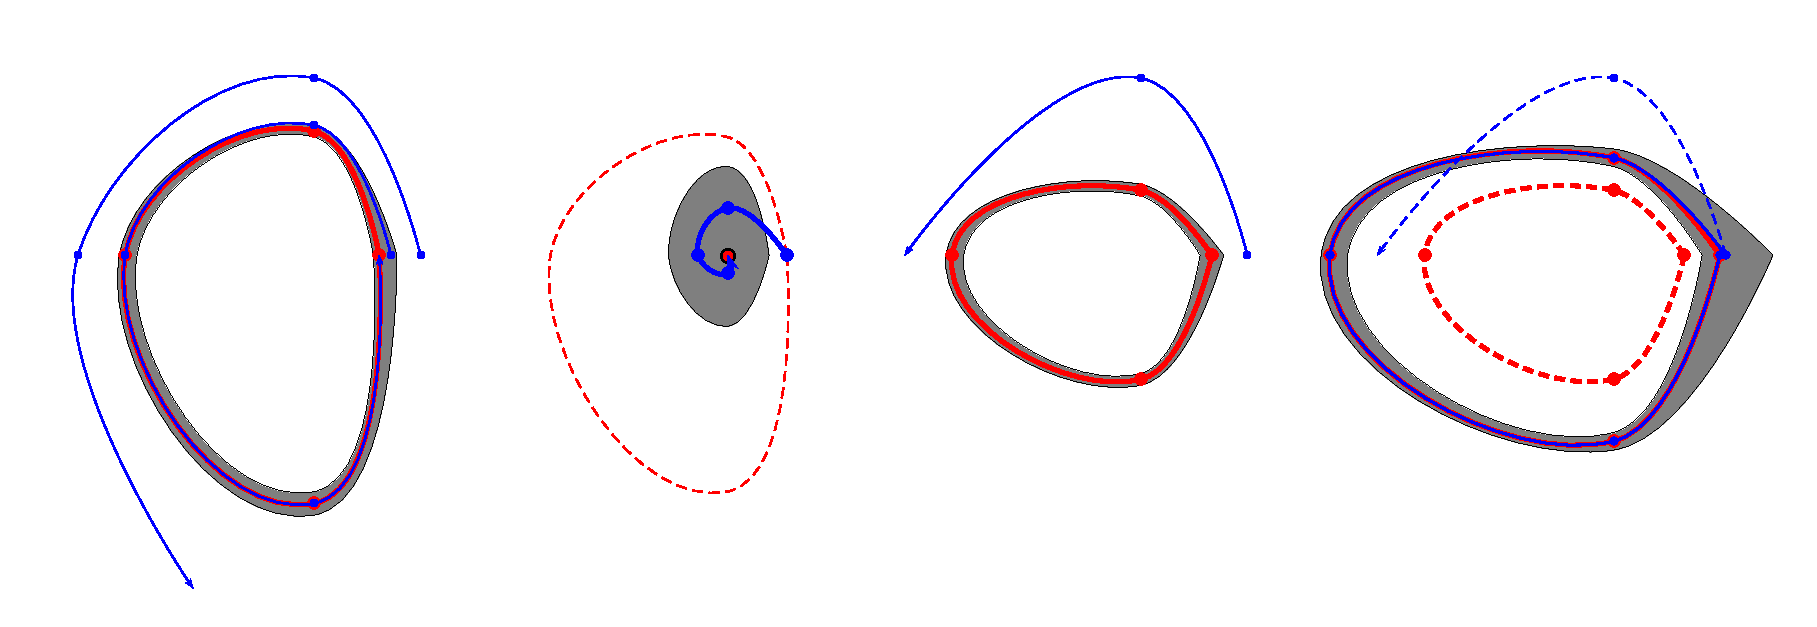
\includegraphics[width=11cm]{images/LimitCircle.eps}}
\caption{Comparison of the results predicted by our models against video of a human iris. (left) One frame of an
animation simulating the changes in pupil diameter and iridal pattern deformation. (center) One frame from a video of a
human iris. (right) Graph comparing the measured pupil diameters from each individual frame of a nine-second-long video
sequence (green line) against the behavior predicted by our model (red line). The gray bars indicate the periods in which
the light was kept on and off. The complete video sequence and corresponding animation are shown in the accompanying
video.}    
  \label{fig:videocomparison}
\end{figure*}


\subsection{Motor Primitives}
In real life, animals’ motions are result of the dynamic interaction between itself and environment.
In general, dynamic motion can be described with differential equation
\begin{equation}
	\dot{x}=f(x,u)
\end{equation}

Where x is the system state, $\dot{x}$ is the derivative and $u$ is the control signal. 
When u=0, such system are called autonomous system and capture the intrinsic motion property. 
Important properties of motion are shown on phase plot; 
Figure 1 shows a limit circle. 
All the motions converge as time goes on.
\begin{figure}
\end{figure}

The limit of motion is called limit circle and shadow region is called basin of attraction, 
motion within basic attraction converge to the circle.
In real life, all motions should determined limit and stable, the motion must be attractive.
Basically there are two types of limits, periodic and fix point. 
Corresponds the period tic motion and discrete motion.
A motion primitive is defined by its equilibra and its attractivity.

\subsection{Motor Control}
For motion control the key problem comes in two situations.

\textbf{State Perturbations} motion primitive is kept but the initial position is moved out of basin of attraction.
For walking, a push perturbation will have such effect. In motion synthesis, this is the motor control.

\textbf{Structure Perturbation}
Motion primitives can change its shape, type or even attractivity.
comes from changing f. for walking example it may comes from the change of body weight or terrain. This problem in nature is motion retargeting.
Most current idea applying a control to push state back to boa, such controller only applies to S1.

our method is different and  separated in two steps.
(1) Maintain the attractor type and its attractively. The shape is not considered. As in figure 2

(2)Transform the motion primitive on phase plane, to include the state X inside the basin of attraction. As in Figure 3

Thus our framework solved the stable control and motion retargeting problem in a unified way.The shape change of attractor means more adaptive motion results.

In mathematically, the first step is keep the topology of motion primitives or Global Motor Invariant. The transform available is close related to the properties of f, which is the lie symmetry, or the Local Motor Invariant.



Figure 2 Global Invariant Control




Figure 3 Local Motor Invariant Controls and Transformation

\subsection{Motion Transition}
When an character transform from one motion into another, character should in the state space $(q,\dot{q})$
For when motion is translated from motion ma to motion mb.
The state of %$(q,\dot{q} \in Boa(ma) \union Boa(mb)$

\section{Global Motor Invariant and Control}
\subsection{the Qualatitve Property of Motion}
When generating adaptive motion, one key question is what can be adaptive while what must be maintained.
For walking example, people walking in different manner and different way.
But still some key properties are kept unchanged.

A method for modelling the qualitative property can be identified by the topology of phase plot.
For the walking example, some researchers argue that, the key properties of walking or any other kinds of locomotion, is the periodic change of the body shape.
On the phase plot, this means the topology of the phase plot is the same to that of the circle.
The topology of the phase plot is defined as the Global invariant, which determines the qualitative properties of motion.

When keep the topology against the change in system dynamic, this is the structuable stability control, which in nature solves the motion retargeting problem.
When the topology is kept against the perturbation in state, this is the stability control,
Which in nature solves the stalibty control in motion synthesis.

Different kinds of perturbation will generate different shape of phase plot. This is allowed in our framework and even seen as an advantage, because the shape changed reflect the adaptation in motion. 


By the topology,
basically motion can be separated into two group.
1 periodic motion
Some motion show pepetive pattern, from geometrical viewport, on the phaseplane, the attractor of curve form the shape of a circle.
2 discrete motion
Some motion is terminated, from geometrical viewport, on phase phaseplane,  a ttractor is a point.

In this research, we only consider periodic motion. This for two reason, the first one is that some biological research believe that life system itself is peroditic in nature. From application viewport, fix point can be approximate with a limit circle with a small amplitude.

\subsection{Entrainment}
For periodic motion, global controller don’t care about the shape, of oscillation, it only cares about the topology of the phase plot.
The method we prosposed is based on the entrainment.
The basic idea is couple two oscillator together. The dynamic system form one oscillator, while the control system form the other oscillator.
The control system system is topological structural stabile, and oscilate with the mechanical one in an similar manner,
When the mechanical oscillator is disrupted, whe control oscillator will drive the mechanical oscillator return to oscillation model.
Whe control oscillatior we prosed is based on the matusta oscillator.
With the equation of following form.


Stability of Control Oscillation.
Automotous Oscillation
From initial position, matsushiata oscillator all converge to the same limit circle.
Entrainment Oscillation
Matsuta oscillation can coupble with a various oscillator.
\begin{eqnarray}
\tau_{1} \dot{x_{1}}&=&c-x_{1}-\beta v_{1}-\gamma [x_{2}]^{+}-\sum_{j}h_{j}[g_{j}]^{+}\\
\tau_{2} \dot{v_{1}}&=&[x_{1}]^{+}-v_{1}\\
\tau_{1} \dot{x_{2}}&=&c-x_{2}-\beta v_{2}-\gamma [x_{1}]^{-}-\sum_{j}h_{j}[g_{j}]^{-}\\
\tau_{2} \dot{v_{2}}&=&[x_{2}]^{+}-v_{2}\\
y_{i}&=&\mbox{max}(x_{i},0)\\
y_{out}&=&[x_{1}]^{+}-[x_{2}]^{+}=y_{1}-y{2}
\label{eq:matsuta}
\end{eqnarray}
\chapter{LOCAL MOTOR INVARIANT}
\label{chap:li}

\nomenclature[f1]{$G$}{A Lie Group}
\nomenclature[f2]{$g_a$}{an element in Lie Group $G$ with parameter $a$}
\nomenclature[f3]{$I(x)$}{Invariant Function of $x$}
\nomenclature[f4]{$\ep$}{The parameter of a lie group element}
\graphicspath{{LocalInvariant/LocalInvariantFigs/EPS/}{LocalInvariant/LocalInvariantFigs/}}
It is not enough that animals are able to maintain the global motor invariant.
For a fish, preserving \emph{Global Motor Invariant}  means the swimming is stable and can be sustained.
However,  a fish also needs to adjust the speed and direction during swimming, which is of crucial importance for survival.
In real-life, animal can adapt motion primitives according to its purpose precisely.
In this chapter, we will develop the control strategies for tweaking motion patterns according to the motion purposes.

It is important to remember that such tweaking strategies are also constrained by the computation and memory capacity of the neural system, and should explore natural dynamics as the basic motion primitive theory. 
For \cms, it is of no meaning developing walking pattern by exploring natural dynamics but using optimization to adjust the walking speed. 
To meet such requirements, \moit\ adopted different ideas.

At first, when tweaking motion patterns, stability should not be violated. 
As stated in the previous chapter, a topological conjugation (one-one continuous invertible mapping)maintains the topology thus maintains the qualitative stability. Thus the ``tweaking'' action should be a topology conjugation. In an alternative perspective, such operations form a group and permit a combination operation. 

According to Group Theory, this means if two tweaking actions preserve the stability separately, the combination of the two actions also preserve the stability.
The space of topology conjugation is very large.
Currently, \moit\ only investigates a subset called \emph{The Lie Transformation Group} that is supported by the biological research studies and can be calculated efficiently.
The selected groups can be divided into orthodox subgroups, each of which is continuous and can be parameterized by one parameter.
In \cms, such parameters are closely related to motion purposes such as walking speed or swimming direction.

From the dynamic perspective, ``tweaking''  should also explore natural dynamics (passive based) as primitives.
Methods adopted in \moit\ belong to  a popular passive-based control principle, which carries many names: Controlled Symmetry, Controlled Lagrange, or Potential Shaping.
Different names reflect the fact that this method can be developed through different ways.
Roughly speaking, the original dynamic system is transformed according to motion purpose, the kinematics is untouched and control is applied by modifying the potential energy.
Such methods suit biological actuators like muscles and are also computationally efficient:
Closed form formula are developed for converting tweaking parameters to control effort.

This chapter is laid out in this way:
Section~\ref{sec:groupandsymmetry} introduces the basic idea of group and symmetry from intuitive geometry examples to more abstract algebraic formulation. Section~\ref{sec:liecontrol} investigates application of the Controlled Lagrange Method.
At last an example is provided in Section~\ref{sec:symball} to illustrate the idea.

In theory the ideas of group and invariant are closely related, like the two sides of a coin.
Group are the transformations which keep certain property invariant.
When searching for the group transformation, the invariant property is also determined.

In Motor Invariant Theory, the quantitative properties that are  preserved during group transformation are called \emph{Local Motor Invariant}.







\section{Group and Symmetry}
\label{sec:groupandsymmetry}
%To make motions realistic, some natural looking features should also be preserved.
%Some features of motions such as smoothness or energy efficient are quantitative.
%\cms research should provide a framework preserving feature.
%Another question mission is animals can finish motion tasks require high accuracy.
%
%These are the motivations for the development of \emph{Local Motor Invariant}.
%Local Motor Invariants are quantitative properties of motions, the idea of invariant preserving are abstracted as the ``Symmetry'' and Group theory.
%Features are modelled as symmetrical functions, while feature preserving actions form a group.
%From dynamic perspective, motions are solutions to dynamic equations.
%The actions transform one motion to another close related to the Lie Group Theory for differential equations\citep{olver1986applications}.
%
%The introduction of Lie Group not only provides a powerful mathematical tools for modelling the symmetry property, but also provides an idea to simplify the solving the dynamics.



For the more traditional geometrical perspective, ``Symmetry''  means a geometry is the same after certain transformation.
For example, a square remains the same shape after  $90$ degree clockwise rotation, as shown in Figure~\ref{fig:symsquare}.
\begin{figure}[!htbp]
  	\begin{center}
   	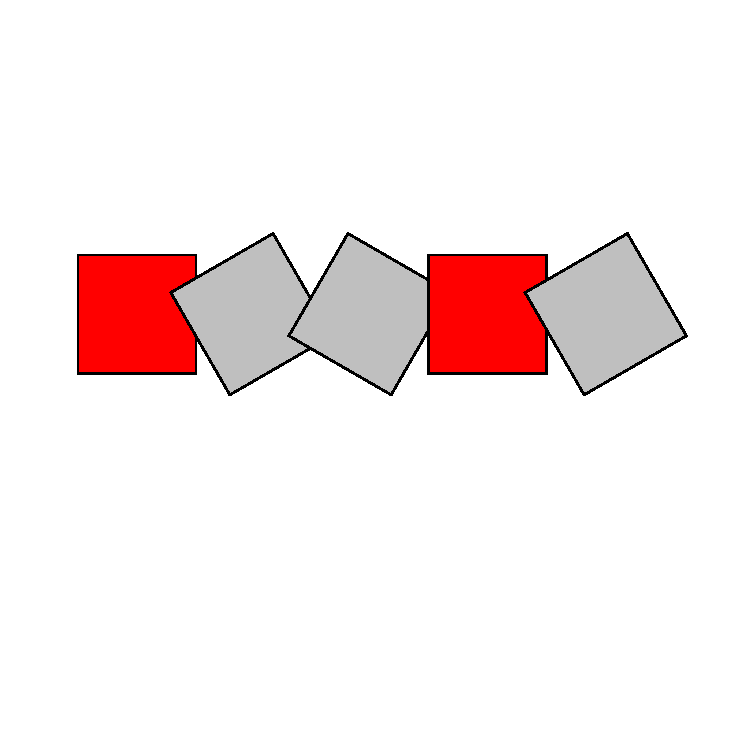
\includegraphics[width=0.5\textwidth]{SquareRotate}
	\end{center}
	\caption{Symmetry of The Square}
    \label{fig:symsquare}
\end{figure}

Actions that preserve the square shape can be combined.
For example, if the action of $90$ degree clockwise rotation preserves the shape, then the action of rotating twice, i.e., $180$ degree clockwise rotation also preserves the shape.

All the actions that can preserve the symmetry form a group $G$.
A group has the following properties.
\begin{enumerate}
\item For any $g_a,g_b$ in $G$, \,$g_a*g_b$\, belongs to $G$. (The operation ``$*$'' is closed).

\item For any \,$g_a,g_b,g_c\in G$, \,$(g_a*g_b)*g_c=g_a*(g_b*g_c)$. \,(Associativity of the operation).

\item There is an element $e\in G$ such that \,$g_a*e=e*g_a=g_a$\, for any \,$g_a\in G$. (Existence of identity element).

\item For any \,$g_a\in G$\, there exists an element $g_h$ such that \,$g_a*g_h=g_h*g_a=e$. \,(Existence of inverses).
\end{enumerate}

For the square example, all the actions preserve the square shape form the group $G$.
$g_1$ is  $90$ degree clockwise rotation, identity element $e$ is the action of no rotation,
$g_2=g_1*g_1$ is the action of rotating $90$ degree clockwise twice.
Since $g_2$ preserves symmetry, $g_2$ is an element of the group $G$, 


From the algebraic perspective, ``Symmetry'' means the value of function is invariant after transformation.
For a function $I(x)$,
the group transformation is define by $\tilde{x}=g_a(x)$.
By symmetry, we mean $I(x)=I(\tilde{x})$.
$I(x)$ is an invariant function of group $G$.


Note that  shapes invariant by actions in $G$  are not unique.
Many shapes are invariant, and their combinations are also invariant, as shown in Figure~\ref{fig:SymmetrySpace}. 
In the algebraic sense,  invariant functions of group $G$ form a space, the invariant space $I^G$.


\begin{figure}[!htbp]
  \begin{center}
    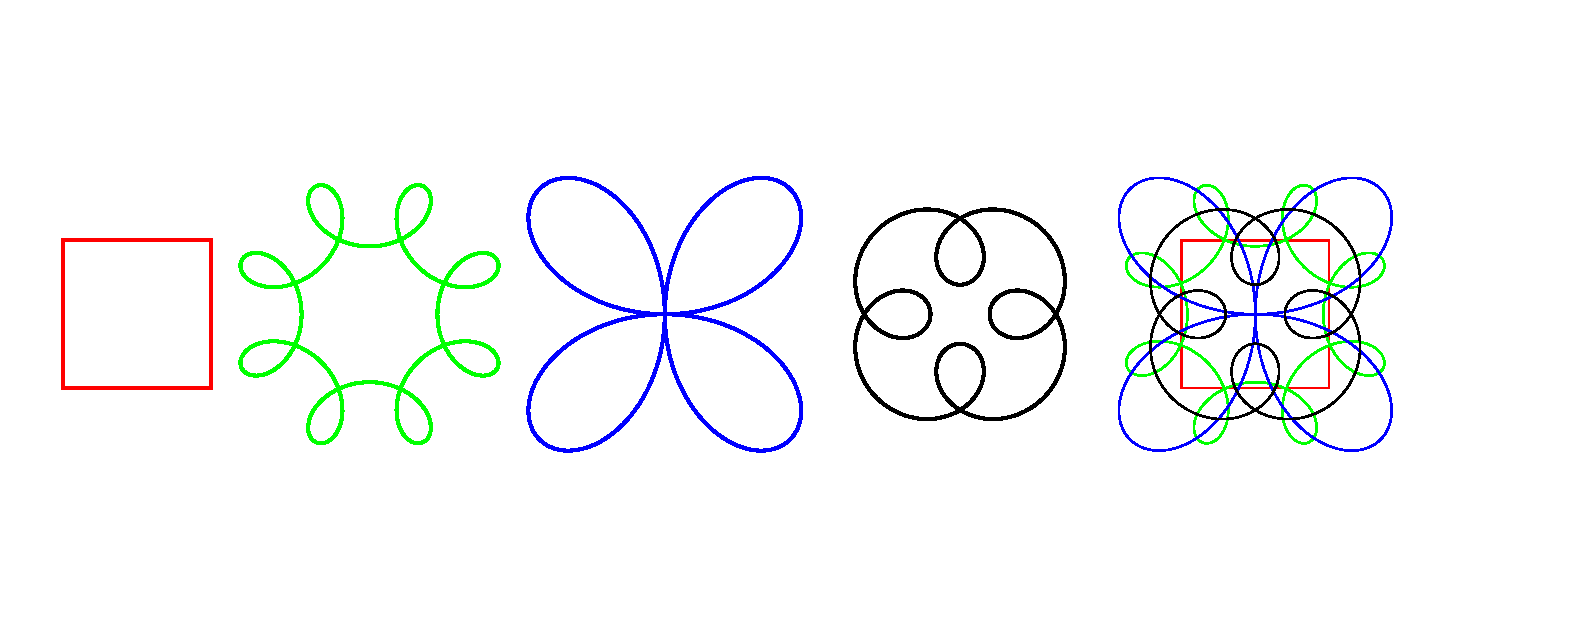
\includegraphics[width=0.7\textwidth]{ShapeCombination}
    \caption{Two invariant Shapes and the invariant combination}
    \label{fig:SymmetrySpace}
\end{center}
\end{figure}

\subsection{Lie Group and Differential Equation}
Physically-based motions are usually described by differential equations, and motion is the solution of the equation.
Same as the square shape, there are also symmetry groups that keep the differential equations invariant.
An important property of such a group  is that its elements can transform the solution of differential equations from one into another\citep{olver1986applications}.
For \cms, this property  can potentially help reduce computational burden: new motions can be achieved through applying  transformation to the dynamic equations of motion primitives.




In mathematical theory, \emph{Lie Group} is continuous group, which is also a manifold.
Since it is a manifold, coordinate system can be assigned to a Lie Group and each elements can be parameterized.
For example, the symmetry rotation group of square is discrete, while symmetry group of circle is continuous.
For the symmetry group of the circle, each element can be parameterize by the the rotation angle.
In the following discussions,  $\ep$ is the parameter of a element $g$ in the group $G$.

Theory of Lie group comes from the study of differential equations.
For the differential equation in Equation~\ref{eq:difforg}.
\begin{equation}
\label{eq:difforg}
\dot{\state}=F(\state)
\end{equation}
Invariant function $I$ can be defined as:
\[
I(t,\state,\dot{\state})=F(\state)-\dot{\state}
\]
Solutions of the differential equation are the kernel of the invariant function $I$ :
 \[
 I(t,\state,\dot{\state})=0
 \]
 
 
The group transformation will act on all the variables of the invariant function.
Therefore $t$, $\state$ and $\dot{\state}$ are all transformed.
\[
(t,\state,\dot{\state}) \mapsto (\tilde{t},\tilde{\state},\dot{\tilde{\state}})
\]
If the group $G$ is symmetrical, then value of the  function $I$ will be invariant.
Therefore  the kernel is transformed into kernel, and the transformed variables are still solutions to the original differential equations. 
\[
I(t,\state,\dot{\state})=I(\tilde{t},\tilde{\state},\dot{\tilde{\state}})=0
\]


Note that the $\dot{\state}$ is not independent which depends on the $t$ and $\state$,
\[
\dot{\tilde{\state}}=\frac{d \tilde{\state} }{d \tilde{t}}
\]
From the geometrical perspective, it is not easy to present  the transformation of $t$.
Instead, we define two actions on the state space and tangent space.
In the state space, we define the  action $g$ that transforms the state. 
\[
g(\state)=\tilde{\state}
\]
In the tangent space, we define the \emph{lift action} $Tg$ 
\[
Tg(\dot{\state})=\dot{\tilde{\state}}
\]

$Tg$ can be worked out by formatting the derivatives in the original coordinate system.
For example, the translation $g_{\ep}$ 
\[
(x,y)\mapsto (x+\ep,y+\ep)
\]
$Tg_{\ep}$ is
\[
(\dot{x},\dot{y}) \mapsto (\dot{x},\dot{y})
\]
$Tg$ is the identity element $e$.


In the general cases, $g$ transforms Equation~\ref{eq:difforg} into Equation~\ref{eq:trdiff}
\begin{equation}
\label{eq:trdiff}
Tg(\dot{\state})=F(g(\state))
\end{equation}
If $g$ is symmetrical, Equation~\ref{eq:difforg} and Equation~\ref{eq:trdiff} are equivalent







 	
For example, 
The scaling action is applied to the state space of the mass spring system of Equation~\ref{eq:stateform}. 
\[
\tilde{\state}=g_{\ep}(\state)=[\ep q, \ep \qd ]
\]
then the lift action is
\[
\tilde{\state}=Tg_{\ep}(\state)=[\ep \qd, \ep \ddot{q}]
\]



by substitution $\state \mapsto \tilde{\state}$, the original system becomes
\[ 
\dot{\tilde{\state}}=
\left[ 
\begin{array}{cc}
0 &1\\
-1 &0 
\end{array}
\right]\tilde{\state}
\]
which is 
\begin{equation}
\label{eq:tranmas} 
\ep \dot{\state}=
\left[ 
\begin{array}{cc}
0 &1\\
-1 &0 
\end{array}
\right]\ep \state
\end{equation}

Equation ~\ref{eq:tranmas} is equivalent to  Equation~\ref{eq:stateform}.
If $\state(t)$ is a solution, so is $\tilde{\state}(t)$.

To verify the group property. define $*$ as:
\[
g_{\ep_1}*g_{\ep_2}(\state)=[\ep_1 \ep_2 q, \ep_1 \ep_2 \qd]
\]

The inverse is:
\[
g_{\ep}^{-1}=g_{\frac{1}{\ep}} \;\ep \in R^+
\]

\begin{mydef}
For a group $G$, the invariant function of state $I(\state)$ is called a \emph{local motion invariant} of $G$. 
\end{mydef}

Invariant functions $I(\state)$ has important  meaning in dynamics. 
According  to \textbf{Noether's Theorem}, each $I(\state)$ corresponds to a conservative law. 


\section{Lie Group and Controlled Lagrange}
\label{sec:liecontrol}
It is not enough for animals  only to  explore symmetry groups of natural dynamics for motion adaptation.
For a dynamic system, the symmetry group is quite restricted.  
Working out the symmetry group might be a non-trivial task.
In real-life, animals usually exert control effort during motion adaptations.

\moit\ theory proposes the idea that control effort can make a non symmetrical group become symmetrical, and introduce the \emph{Controlled Lagrange} technique.
Based on biological research\citep{flash2007affine}, some simple groups are selected the symmetry group for motor control.
When such group is applied to the dynamic system, control efforts are applied to ensure the symmetry.


Usually a dynamic system is represented as by Euler-Lagrange Equation~\ref{eq:uncontrolled_euler_lagrange}\citep{Goldstein2002}.
\begin{equation}
\frac{d}{dt} \frac{\partial L}{\partial \qd} - \frac{\partial L}{\partial q} = 0
\label{eq:uncontrolled_euler_lagrange}
\end{equation}

where $L=K-V$, $L$ is the Lagrange, $K$ is the kinetic energy, $V$ is the potential energy, $q$ is the generalized coordinates, and $\qd$ is the generalized velocity.

By applying the group transformation $g$, both the generalized coordinates and generalized velocity will be changed:
\[
g(\state)=\tilde{\state}=[\tilde{q}, \dot{\tilde{q}}]
\]
The Euler-Lagrange equation for the transformed dynamic system is described by Equation~\ref{eq:liegroup_euler_lagrange}.
If control is applied, the Euler-Lagrange equation of the controlled dynamics is described by Equation~\ref{eq:controlled_euler_lagrange}. 
If symmetry is persevered, the two equation should be equivalent.
Then symmetry control input $\ulocal$ can be calculated by comparing the two equations.
\begin{align}
\frac{d}{dt} \frac{\partial L}{\partial \dot{\tilde{q}}} - \frac{\partial L}{\partial \tilde{q} }&=0,\label{eq:liegroup_euler_lagrange}\\
\frac{d}{dt} \frac{\partial L}{\partial \qd} - \frac{\partial L}{\partial q}&=\ulocal. \label{eq:controlled_euler_lagrange}
\end{align}

When the two equations are equivalent, their Lagrange $L$, Kinetic Energy $K$ and potential energy $V$ should be the same or of the same scale factor.
Thus in theory, two strategies exist and will result in two different $\ulocal$:
we can calibrate the kinetic by scaling and apply control effort to compensate the difference in potential energy, or calibrate potential energy and compensate the kinetic energy.
\moit\ adopts the potential shaping strategy, for it is computational efficient and suitable for muscle like biological actuators.
As a special case, potential energy shaping for homogeneous group or affine group promises a close form formulation.
Several groups and their potential shaping control effort are as below:



\subsection*{ Offset Action}
Offset actions  modify the generalized coordinate $q$ by a constant, while speed and time remain unchanged.
Given the offset parameter $\ep$, the mapping will be in the following form:
\[
(t,q,\qd) \mapsto (t,q+\ep,\qd)
\]

The corresponding state transformation and lift action are
\begin{align}
\goff(\state) &= [q+\ep,\qd] \\
T\goff(\dot{\state})&=\dot{\state}=[\qd,\qdd]
\end{align}


On the phase plot,  the configuration $q$ is usually represented by the horizontal axis, and the generalized speed $\dot{q}$ is represented by the vertical axis.
From the geometrical perspective, offset actions will move the phase portrait horizontally as shown in Figure~\ref{fig:goff}.

\begin{figure}[!htbp]
  \begin{center}
      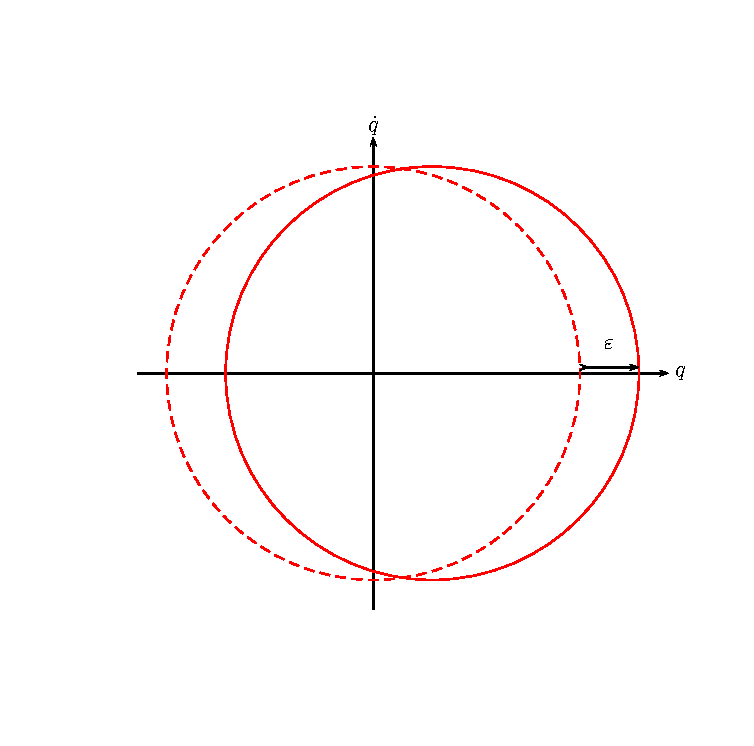
\includegraphics[width=0.5\textwidth]{OffsetAction}
    \caption{Offset Action}
    \label{fig:goff}
\end{center}
\end{figure}

Substituting the transformed $q$ and $\qd$ into Equation~\ref{eq:liegroup_euler_lagrange} and Equation~\ref{eq:controlled_euler_lagrange},
the control input  can be worked out in the following closed form formula:
\begin{equation}
\ulocal(q) = \frac{\partial}{\partial q} \left(V(q)-V(\tilde{q}) \right).
\end{equation}

Taking the mass spring system of Equation~\ref{eq:mass-spring} as an example, the transformed equation  and control equation are as follows.
\begin{align}
\ddot{\tilde{q}}+\tilde{q}-\ep&=0 \nonumber \\
\ddot{q}+q&=\ulocal \nonumber
\end{align}
By comparing the two equations, we work out that:
\[
\ulocal(q)=\ep
\]




\subsection*{Time Scaling}

%g_st(q,dot{q})=(q,st*dot{q})
Time scaling actions divide the time variable by a factor $\ep$.
The generalized coordinates are kept unchanged, and the generalized speed will be multiplied by $\ep$.
For the action of parameter $\ep$, the action mapping is: 


\[
(t,q,\qd) \mapsto (\frac{t}{\ep},q,\ep \qd)
\]

The corresponding state transformation and lift action are
\begin{align}
\gts(\state)&=[q,\ep \qd] \nonumber \\
T\gts(\dot{\state})&=[\ep \qd,\ep^2 \ddot{q}]\nonumber
\end{align}

From a geometrical perspective, time scaling will stretch the phase portrait vertically, as shown in Figure~\ref{fig:gts}.
\begin{figure}[!htbp]
  \begin{center}
    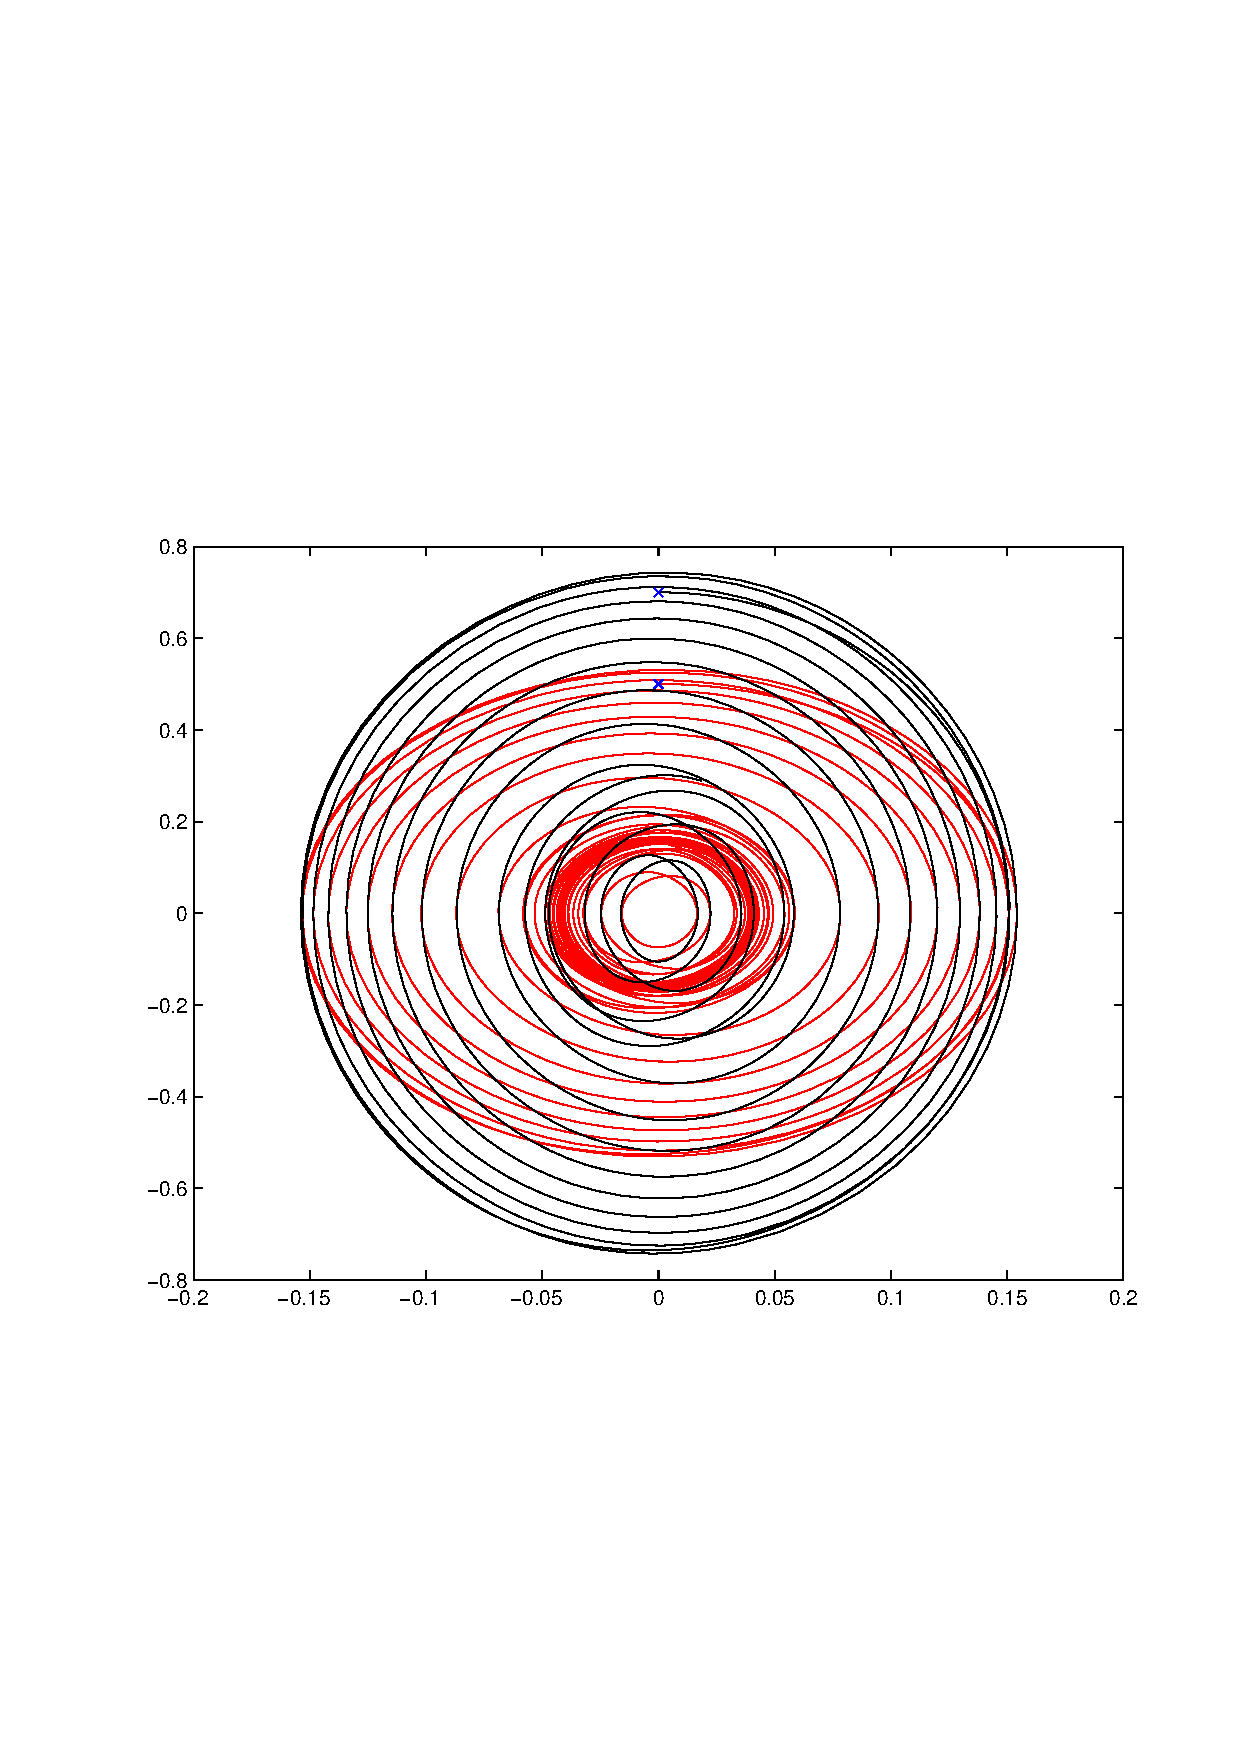
\includegraphics[width=0.5\textwidth]{TimeScaling}
	 \caption{Time Scaling Action}
    \label{fig:gts}
\end{center}
\end{figure}

The control input can be worked out in the same manner as offset actions.
There is also a closed form formula for control input.
\begin{equation}
\ulocal(q) = (1-\ep^2) \frac{\partial V(q)}{\partial q}.
\end{equation}

Again, taking the mass spring system of Equation \ref{eq:mass-spring} as an example, the transformed and controlled equations are

\begin{align}
\frac{\ddot{\tilde{q}}}{\ep^2}+\tilde{q}&=0 \nonumber \\
\ddot{q}+q&=\ulocal \nonumber
\end{align}
The local control input is:
\[
\ulocal=(1-\ep^2)q
\]




\subsection*{Energy Scaling}
For the  dynamic system of the conservative field,
the energy is preserved in motion and different motions are characterized by their energy.
For such a system, motion can be adapted by modifying the energy of the dynamic system.

Energy Scaling action is introduced to adapt motions.
The scaling transformation has the following property:
\[
E(\tilde{\state})=\ep^2 E(\state)
\]
where $E$ is the energy, defined as $E(\state)=K+V$,  $K$ is the kinetic energy, and $V$ is the potential energy.

Further suppose that both the potential and kinetic energy are transformed uniformly.
\begin{align}
K(\tilde{\state})=\ep^2 K(\state) \nonumber\\
V(\tilde{\state})=\ep^2 V(\state) \nonumber
\end{align}
When mass inertia matrix is constant,  the energy scaling transformation is linear as follows:
\[
(t,q,\qd ) \mapsto ( \frac{f(\ep)}{\ep}t ,f(\ep)q,\ep\qd)
\]
$f(\ep)$ is a function of $\ep$, which is determined by the conservative field.
Geometrically, an energy scaling action enlarges the phase portrait,as shown in Figure~\ref{fig:gen}.
\begin{figure}[!htbp]
  \begin{center}
      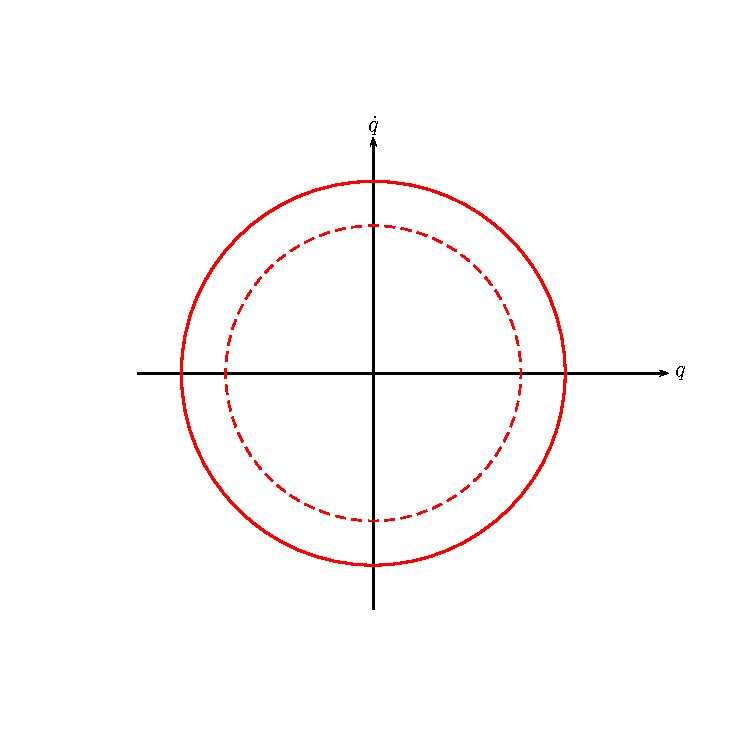
\includegraphics[width=0.5\textwidth]{EnergyScaling}
    \caption{Energy Scaling Action}
    \label{fig:gen}
\end{center}
\end{figure}

The corresponding  state transformation and lift action are:
\begin{align}
\gen(\state)&=(f(\ep) q,\ep \dot{q}) \nonumber\\
T\gen(\dot{\state})&=(\ep \dot{q},\frac{\ep^2}{f(\ep)}\qdd)
\end{align}

$\ulocal$ can by worked out in the same manner as the above actions.
Rather than write down the closed form formula, the thesis prefers an alternative process.
Energy Scaling can be seen as a combined action of two actions: scaling the generalized coordinates and scaling the time variable.
Separate formula can be developed for two actions independently.
This principle generates modular code structure.




The mass spring system of Equation\ref{eq:mass-spring} is selected again as an example.
 For the mass spring system, Energy is defined as~$E=\frac{1}{2}(q^2+\qd^2)$.
 If the energy is scaled up by $\ep^2$,  the potential energy is scaled up by $\ep^2$.
 Because $V= \frac{1}{2}q^2$, and $\ep^2 V=\frac{1}{2}(f(\ep)q)^2$, thus $f(\ep)=\ep$.
 
 
The control input can be worked out in the same manner as the above actions.
However, when object moved in the conservative field, energy scaling is a symmetry group of the original dynamic system, thus no control effort is needed.
\[
\ulocal=0
\]



\subsection*{Time Offset}

Time offset actions modify the time  variable $t$ by the parameter~$\ep$.
The map is as follows
\[
(t,q,\qd) \mapsto (t+\ep,q,\qd)
\]


For a system oscillating with limit cycle, time offset action will modify the phase, as shown in Figure~\ref{fig:gtoff}.
\begin{figure}
  \begin{center}
      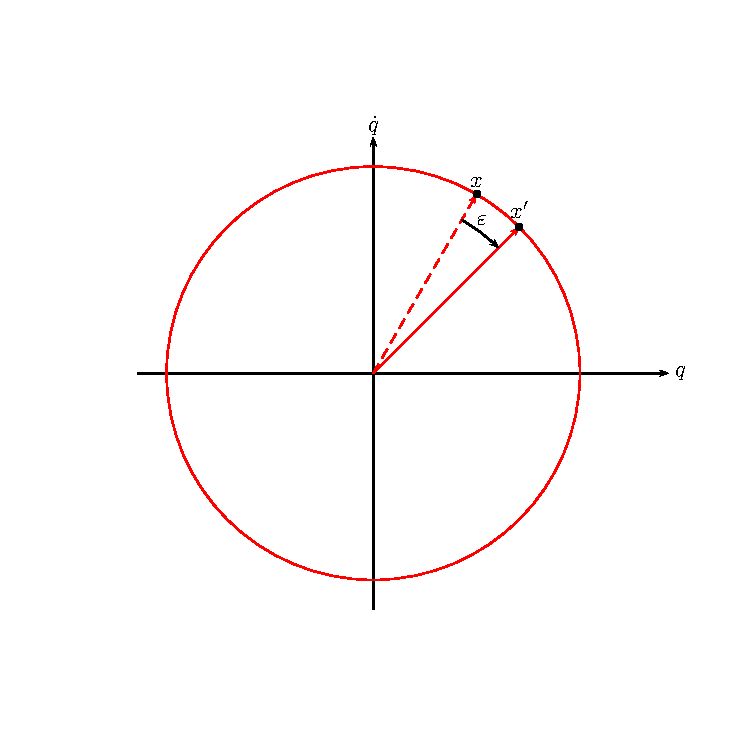
\includegraphics[width=0.5\textwidth]{TimeOffset}
    \caption{Offset Action}
    \label{fig:gtoff}
\end{center}
\end{figure}

For a dynamic system, time offset is symmetrical for all dynamic system.
At the first look, no control effort is needed.
In practise, time offset is achieved by applying time scaling twice, after applying time scaling $\ep$ for sometime, and then apply the inverse action(time scaling of $\frac{1}{\ep}$).


\subsection{Action Selection}
There are many actions available for motion adaptation.
In certain situations, there are many different ways to satisfy the motion constraints, causing the problem which action should be applied.
Different groups will result in different motion styles.
This idea is supported by lots of examples in Chapter~\ref{chap:walk}.
In practise, this is left for the animator to decide.
Usually, the symmetry of natural dynamic is preferred, for such actions are energy efficient.







\section{Example: Symmetry of the Bouncing Ball System}
\label{sec:symball}
Symmetry is a common property among many dynamic systems, even for the hybrid systems like the bouncing ball system of Equation~\ref{eq:bbeq}.
It is shown in this section that by utilizing the symmetry group, complex motions can be predicted in an computationally efficient way.

The bouncing ball system of~\ref{eq:bbeq} has a energy scaling symmetry.

The energy function of the bouncing ball system is  
\[
E=\mathrm{g}q+\frac{1}{2}m\qd^2
\]
If the energy is scaled up by $\ep^2$,  potential energy is scaled up by $\ep^2$.
 Because $V= \frac{1}{2}\mathrm{g}q$, and $\ep^2 V=\frac{1}{2}f(\ep)q$, thus:
\[
f(\ep)=\ep^2
\]
the energy scaling transformation is
\[
\gen(\state)=[\ep^2 q, \ep \qd]
\]

For the bouncing ball system, the energy of a system can be characterized by the initial dropping height.

Given the motion of a ball dropped at $5$ as shown in Figure~\ref{fig:bouncing5}, we set $\ep=\sqrt{2}$ and obtained the motion dropped from $10$ through the transformation as shown in Figure~\ref{fig:bouncing10}.
Figure  motion dropped from $10$ is shown in Figure~\ref{fig:bouncing10sim}.
\begin{figure}[!htbp]
  \begin{center}
      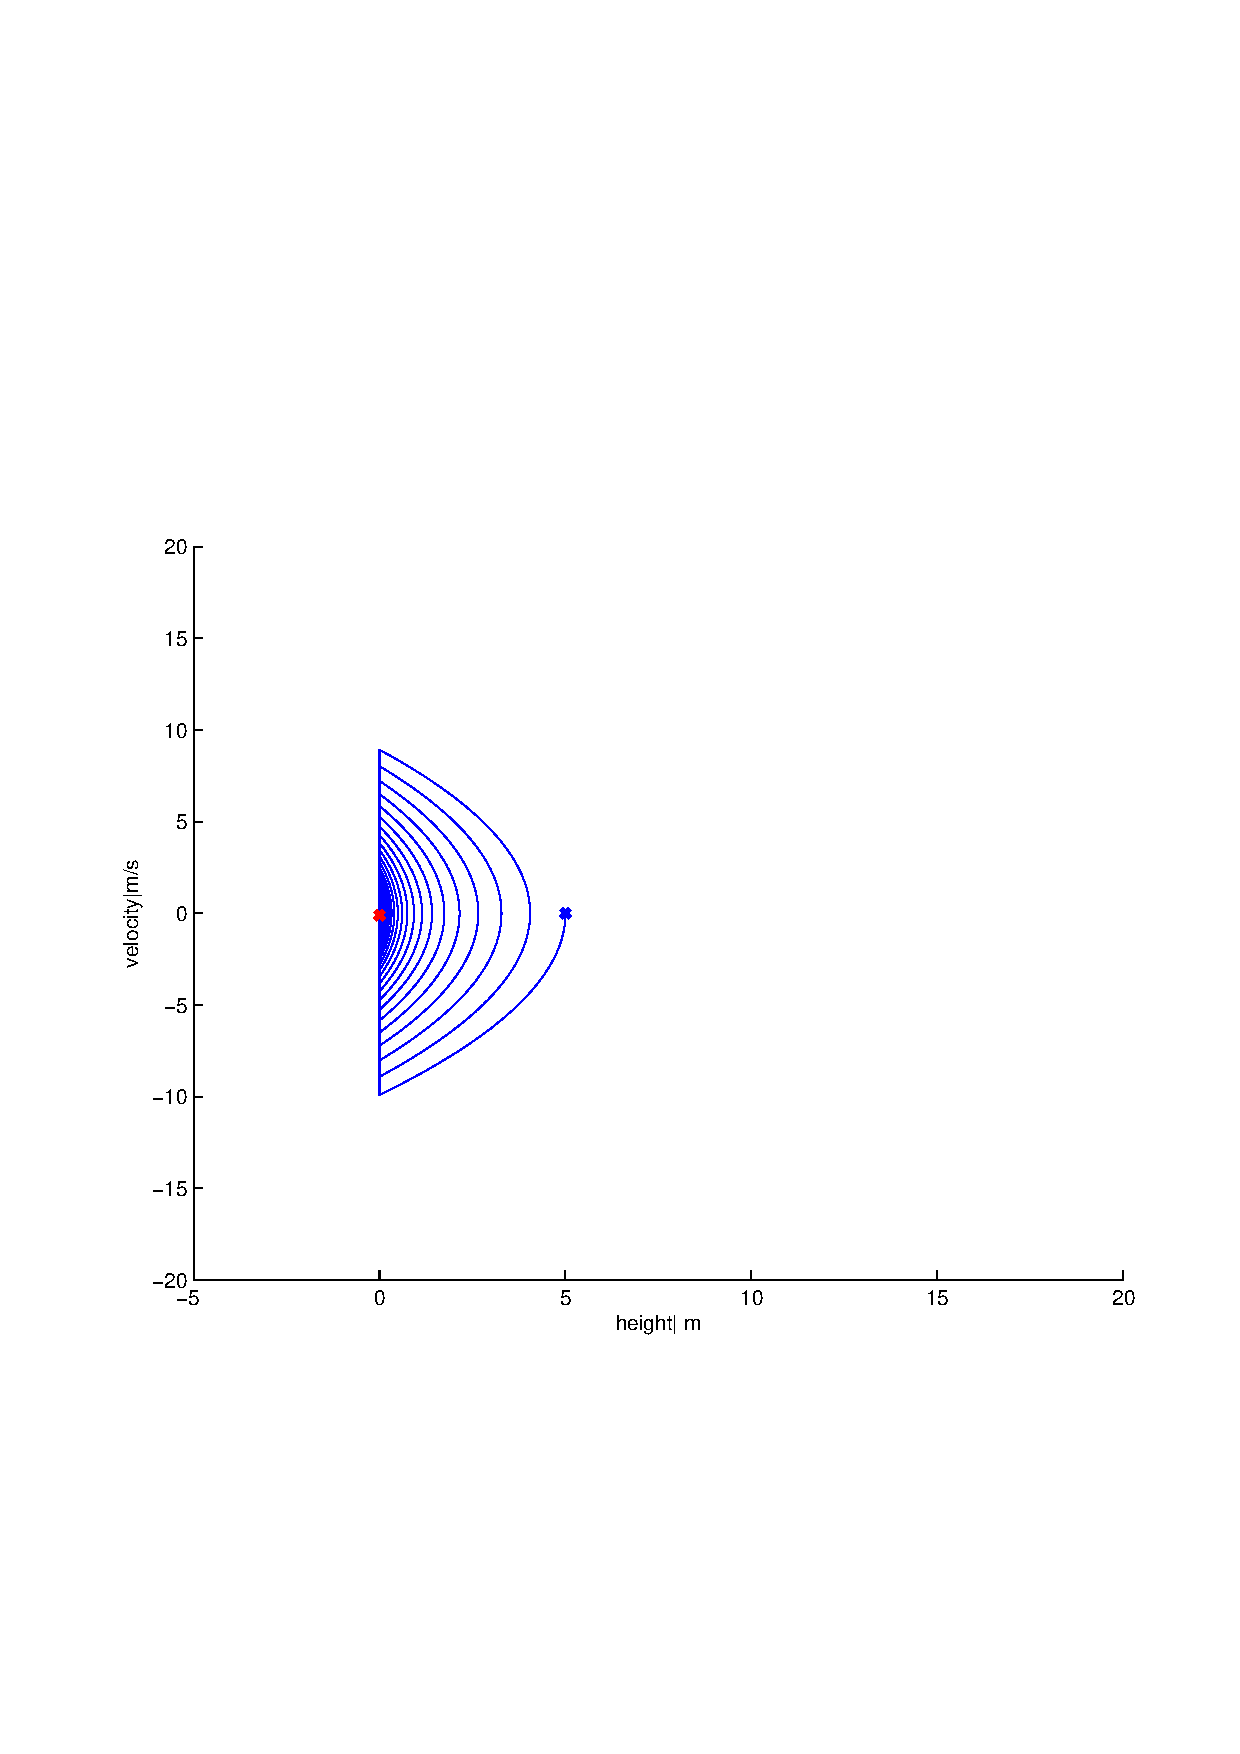
\includegraphics[width=0.5\textwidth]{BouncingBallPhasePlotuncontrolledDropAt5}
    \caption{Drop at 5}
    \label{fig:bouncing5}
\end{center}
\end{figure}


\begin{figure}[!htbp]
  \begin{center}
      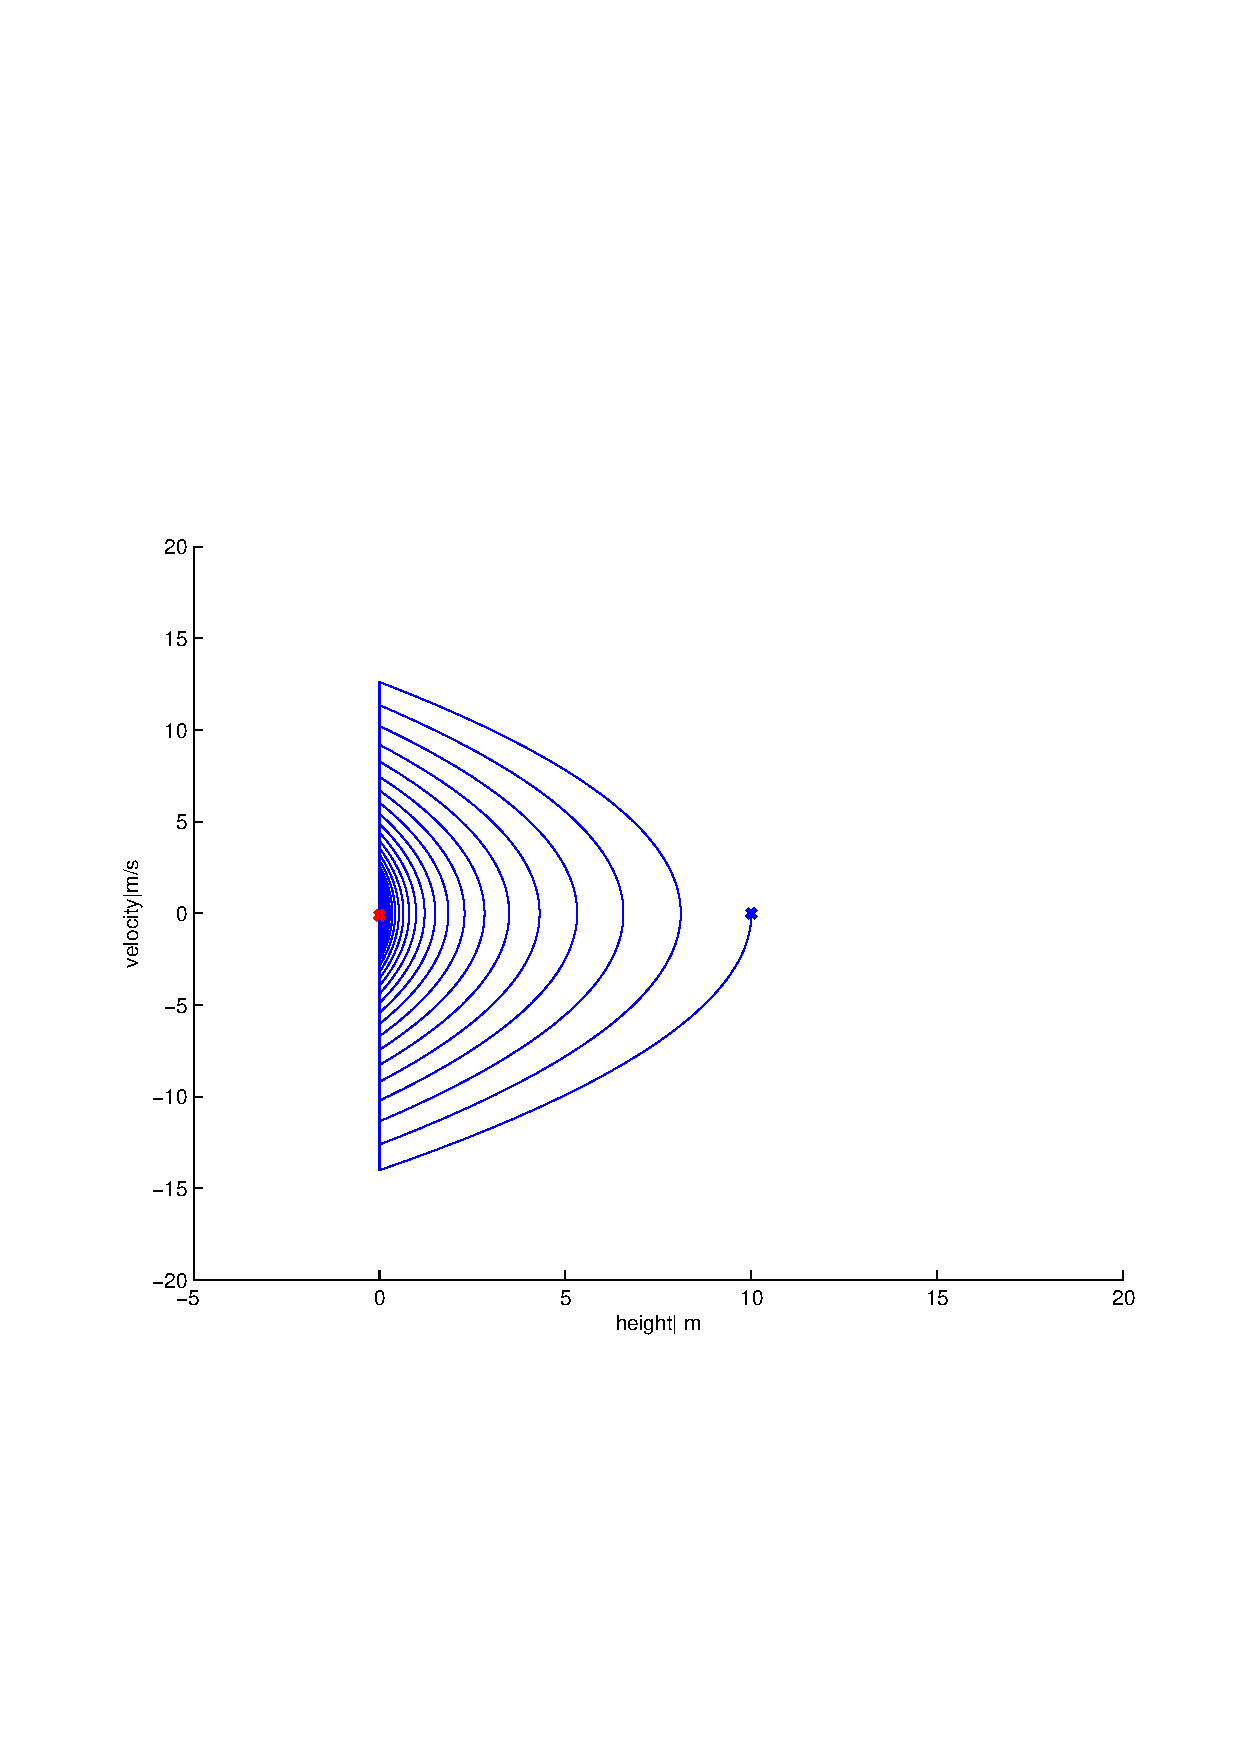
\includegraphics[width=0.5\textwidth]{BouncingBallPhasePlotuncontrolledDropAt10}
    \caption{Drop at 10 by transformation}
    \label{fig:bouncing10}
\end{center}
\end{figure}

\begin{figure}[!htbp]
  \begin{center}
      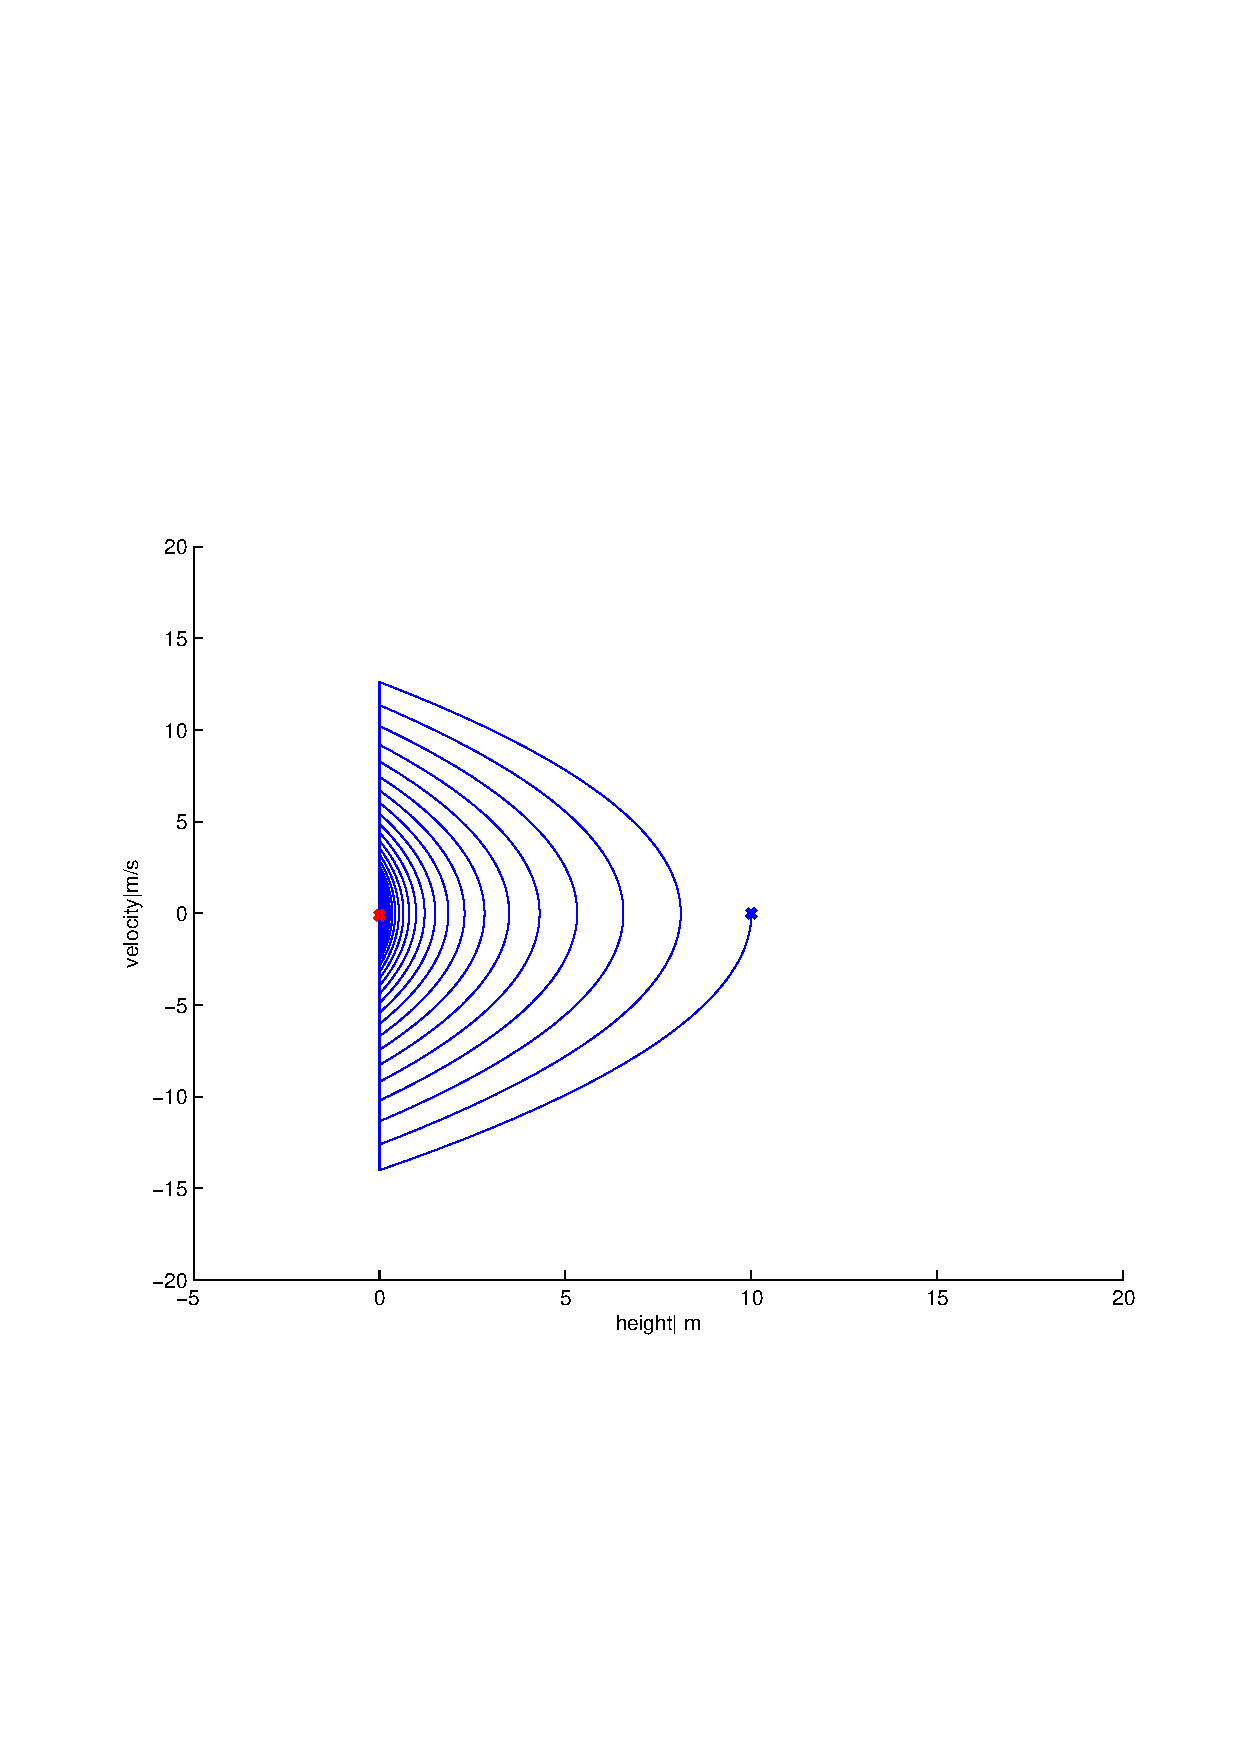
\includegraphics[width=0.5\textwidth]{BouncingBallPhasePlotuncontrolledDropAt10}
    \caption{The simulation result of dropped from 10}
    \label{fig:bouncing10sim}
\end{center}
\end{figure}




\section{Application}
\subsection{Boucing Ball}
\subsubsection*{Dynamic Model}
Bouncing ball is system bouncing by moving a pedal, a system with simple dynamic but difficult to control. 
While this example capture the complexity of human interatction with the environment and object. 
And can be the basic model for many motion tasks, like catch and throw, ball playing, and even walking.

Hybrid dynamics, in incoperate two phase, 
 

%d^2p_ball/dt^2=-g x>0 		p_ball>p_pedal	(1)

%(v_ball-v_mass)=e(v_ball+-v_mass+)	p_vall=p_pedal(2)

Equation (1), is the flying phase equation, equation(2) is the bouncing equation
The -1<e<0.

Basically, the ball will continue bouncing with smaller height.
\subsubsection*{Global Invariant Control}
couple with neural oscillator boucing we get an limit circle
\[g_in=g_in*v_ball, (3)
Pos_pedal=h*out_oscillator.  (4)
\]
The input of neural oscillator is the velocity of the ball multiply by the input coefficient, the output of neural oscillator  drive the pedal position.
An limit circle emerge as the result of entrainment.
As show in figure drop from different position, all the ball will bouncing a about the same height of 5.

\subsubsection*{Local Invariant Control}
Control Bouncing at different Height.
For example boucing at height 10, or 15.
if we define the a*5
the the boucing ball system have energy symmetry.
Controlled Symmetry
If  x(t) is a solution,
So it ax(sqrt(at)) is also a solution

Thus the neural oscillator is modified as follows.
tao=tao*sqrt(a)
out=ta*sqrt(a)
in=in/sqrt(a)

than the a*height is mapped the limit circle.

Following example shows the mapping effect, with a=1, a=3, where the bouncing height is controlled at about height =5 and height =15.
The two pictures are almost the same; this is because the symmetry is perfect.


With Limit Circle At aoubt 15, a=3

With limit circle at about 5, a=1

\subsubsection*{Conclusion}
No matter where the initial position is ,the limit bouncing height can be exactly controlled by modifying the parameters of oscillator.

\subsection{Bipedal Walking}
\subsubsection{Dynamic Model}
iure 1 shows the a two dimensional walking model.
Like bouncing ball, this system is also an hybrid system.
The motion include four phases.
1 in free swing phase.
Mddq/dt+Cdq+N=0
2 the knee strike phase
Qq=Qq
3 the knee lock phase
Mddq/dt+Cdq+N=0
4 the keel strike phase.
Qq=Qq
this system can do passive walking
under specific initial position, the walker can walk passively downstairs.
And exhibit a limit circle.

\subsubsection{Global Invarian Control}
just like mass spring system, the basic idea of control is using the entrainment oscillator to 
motion adaptation. 
The input of the nerual oscillator is the angle between the two legs.
The output of the nerual oscillator is acting on the hip joint
\[
g_in=h*(q1-q2)
yout=hout*neural.
\]
the period is double and the step is not symmetrical any more. So the two legs move in a slight different manner, but still, it keeps walking.

\subsubsection{Local Invariant Control}
lie group symmetry provide method for adapting the walking motion for different terrain and for at different speed.


Slope Change.
N=N*g.
u=N(g*cos(theta)-g)
Speed Change
u=Ng*(speed*speed-1)

4 Walking on any slope with any speed with any walking style
when Combined together, our system can walking on different terrian with any speed and any style.

\chapter{MOTION PRIMITIVE TRANSITION:WALK AND STANCE}
\label{chap:stance}
\ifpdf
    \graphicspath{{WalkStance/WalkstanceFigs/PNG/}{WalkStance/WalkStanceFigs/PDF/}{WalkStance/WalkStanceFigs/}}
\else
    \graphicspath{{WalkStance/WalkStanceFigs/EPS/}{WalkStance/WalkStanceFigs/}}
\fi



\section{Motion Primitives}
For Bipedal Walking, when the heel strike happens, it the passive walker don't get enough velocity, it will stop walk and rest at the heel strike pos.
This is posture is stable, then we got another motion primitive: the stance, as show in figure ~\ref{bipedalstance}



\begin{figure}[!htbp]
  \begin{center}
    \leavevmode
    \ifpdf
      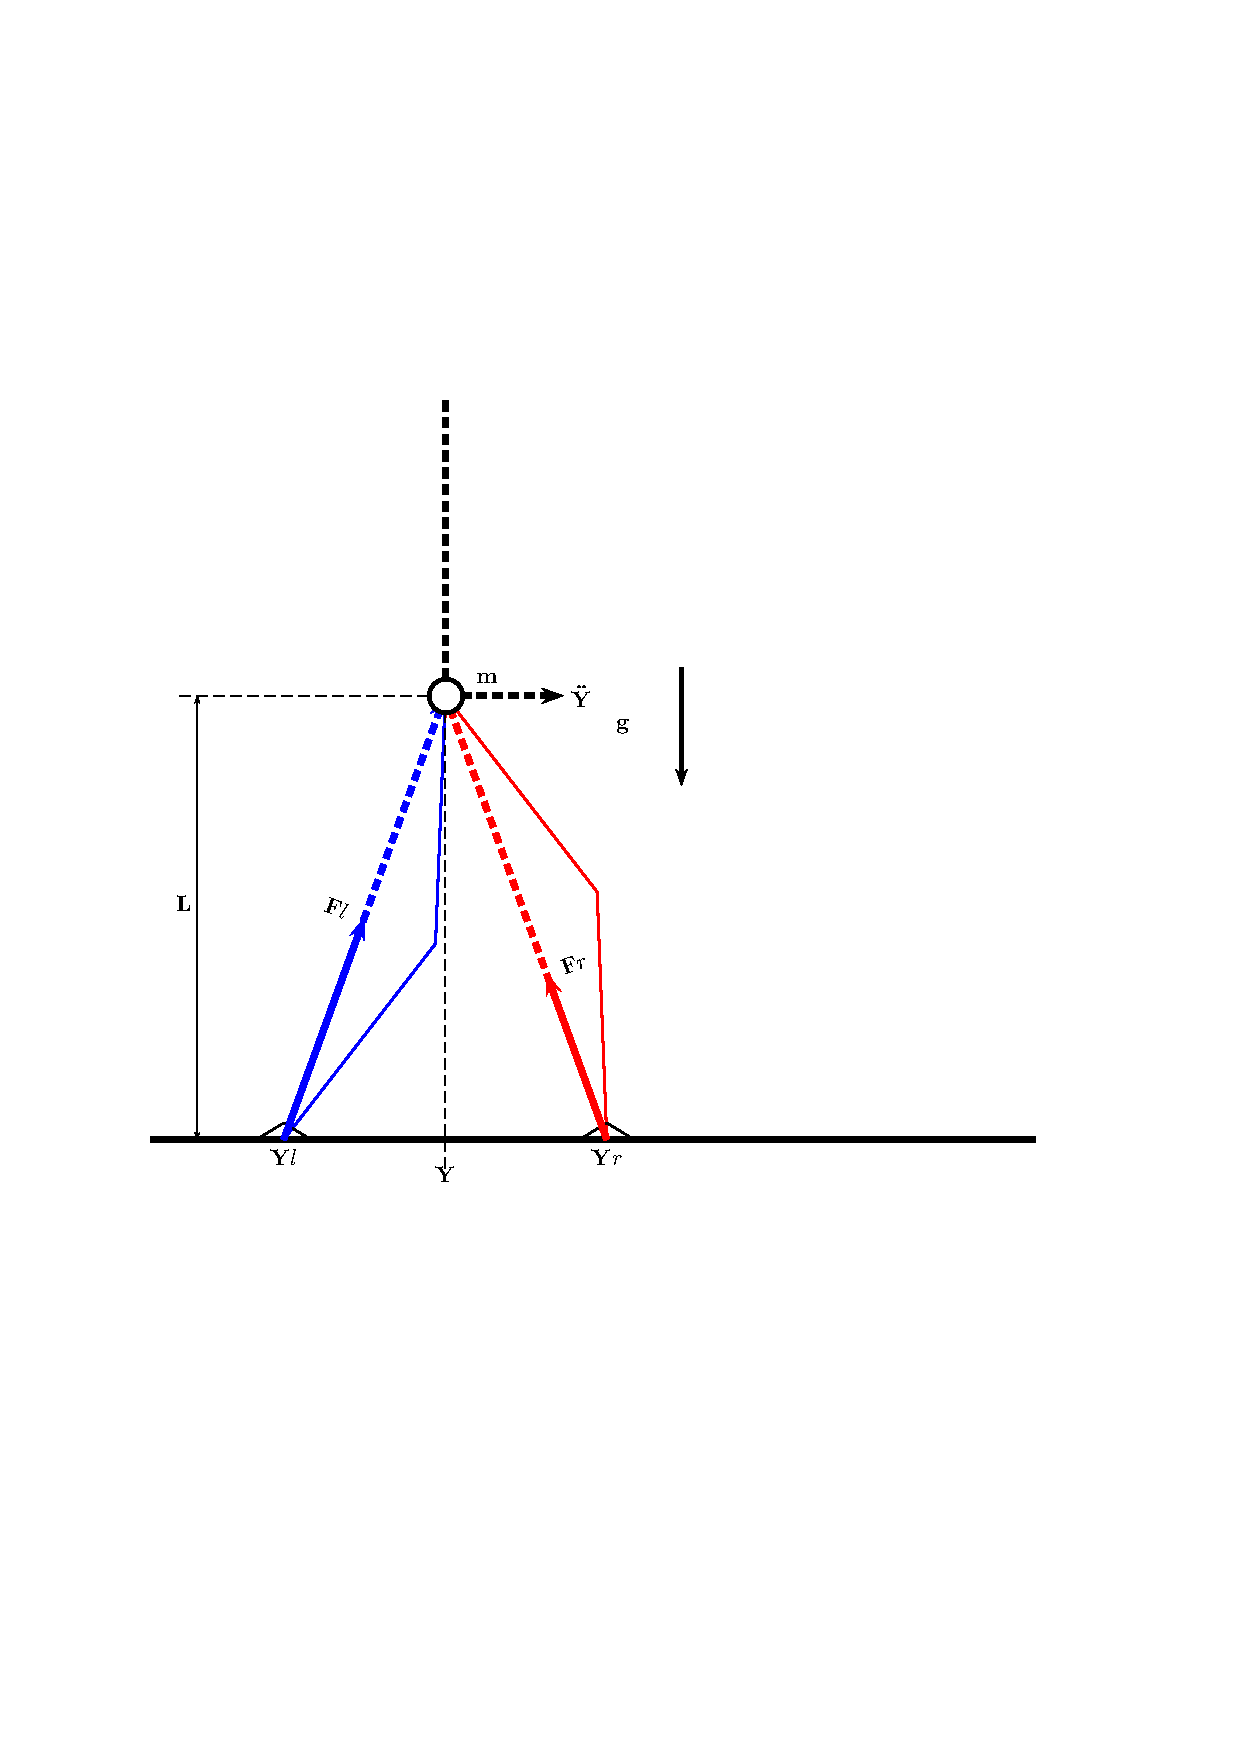
\includegraphics[height=6in]{stancefigure}
    \else
      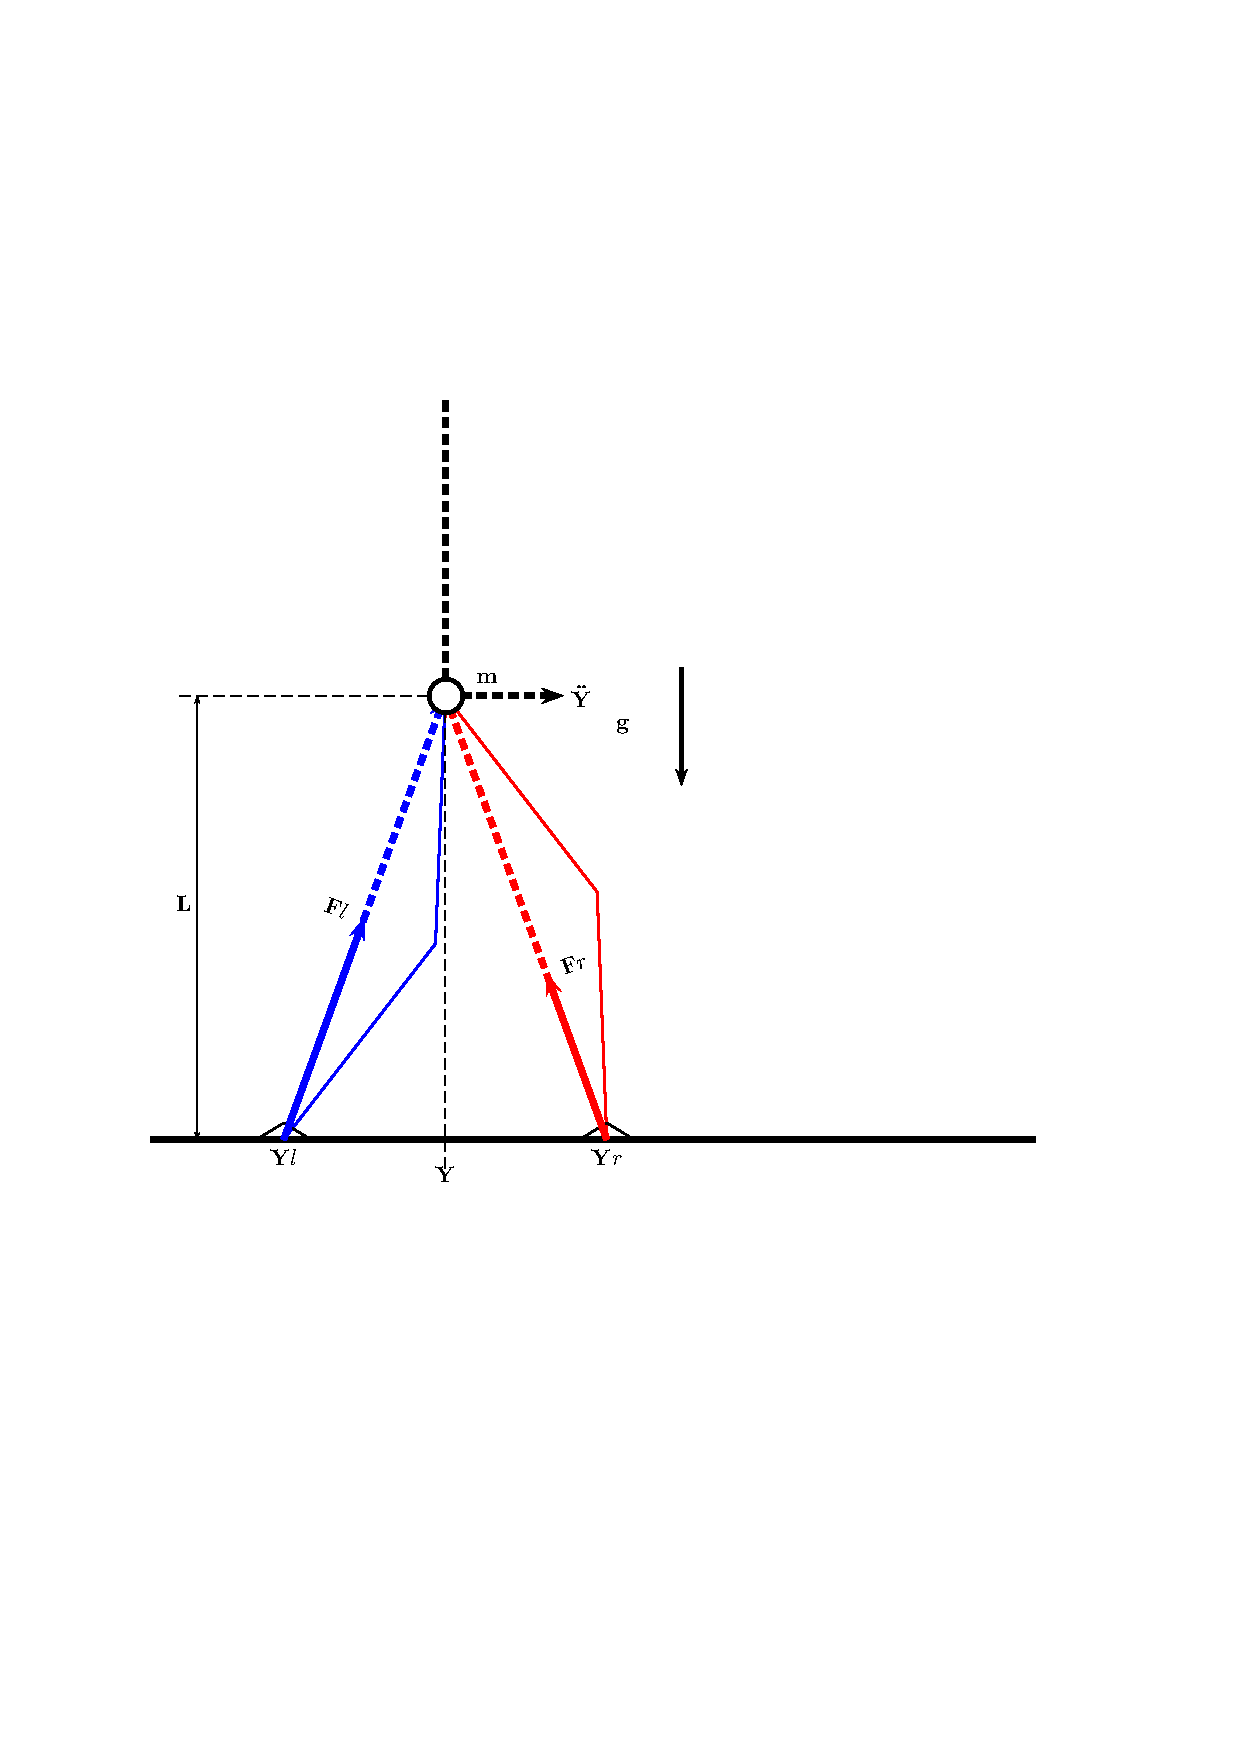
\includegraphics[width=0.7\textwidth]{stancefigure}
    \fi
    \caption{The Stance Motion Primitives}
    \label{fig:bipedalstance}
\end{center}
\end{figure}



usually when people stands, the two legs are almost straight, and the heigt is almost constant.
It is not nessary to consider the full details of four link leg model.
we can simpliy the stance mode as a point supported by two straight legs. 
For normal human stance, high change will be less than 5\%, we suppose it is constant.
we only consider the horizontal displacement.
this simplified model is proposed by although is simple, but capture the key characters of stancing~\citep{stephens2009modeling}.
use this method, we show the stance motion in the following figures ~\ref{fig:stanceopostures}

\begin{figure}[!htbp]
  \begin{center}
    \leavevmode
    \ifpdf
      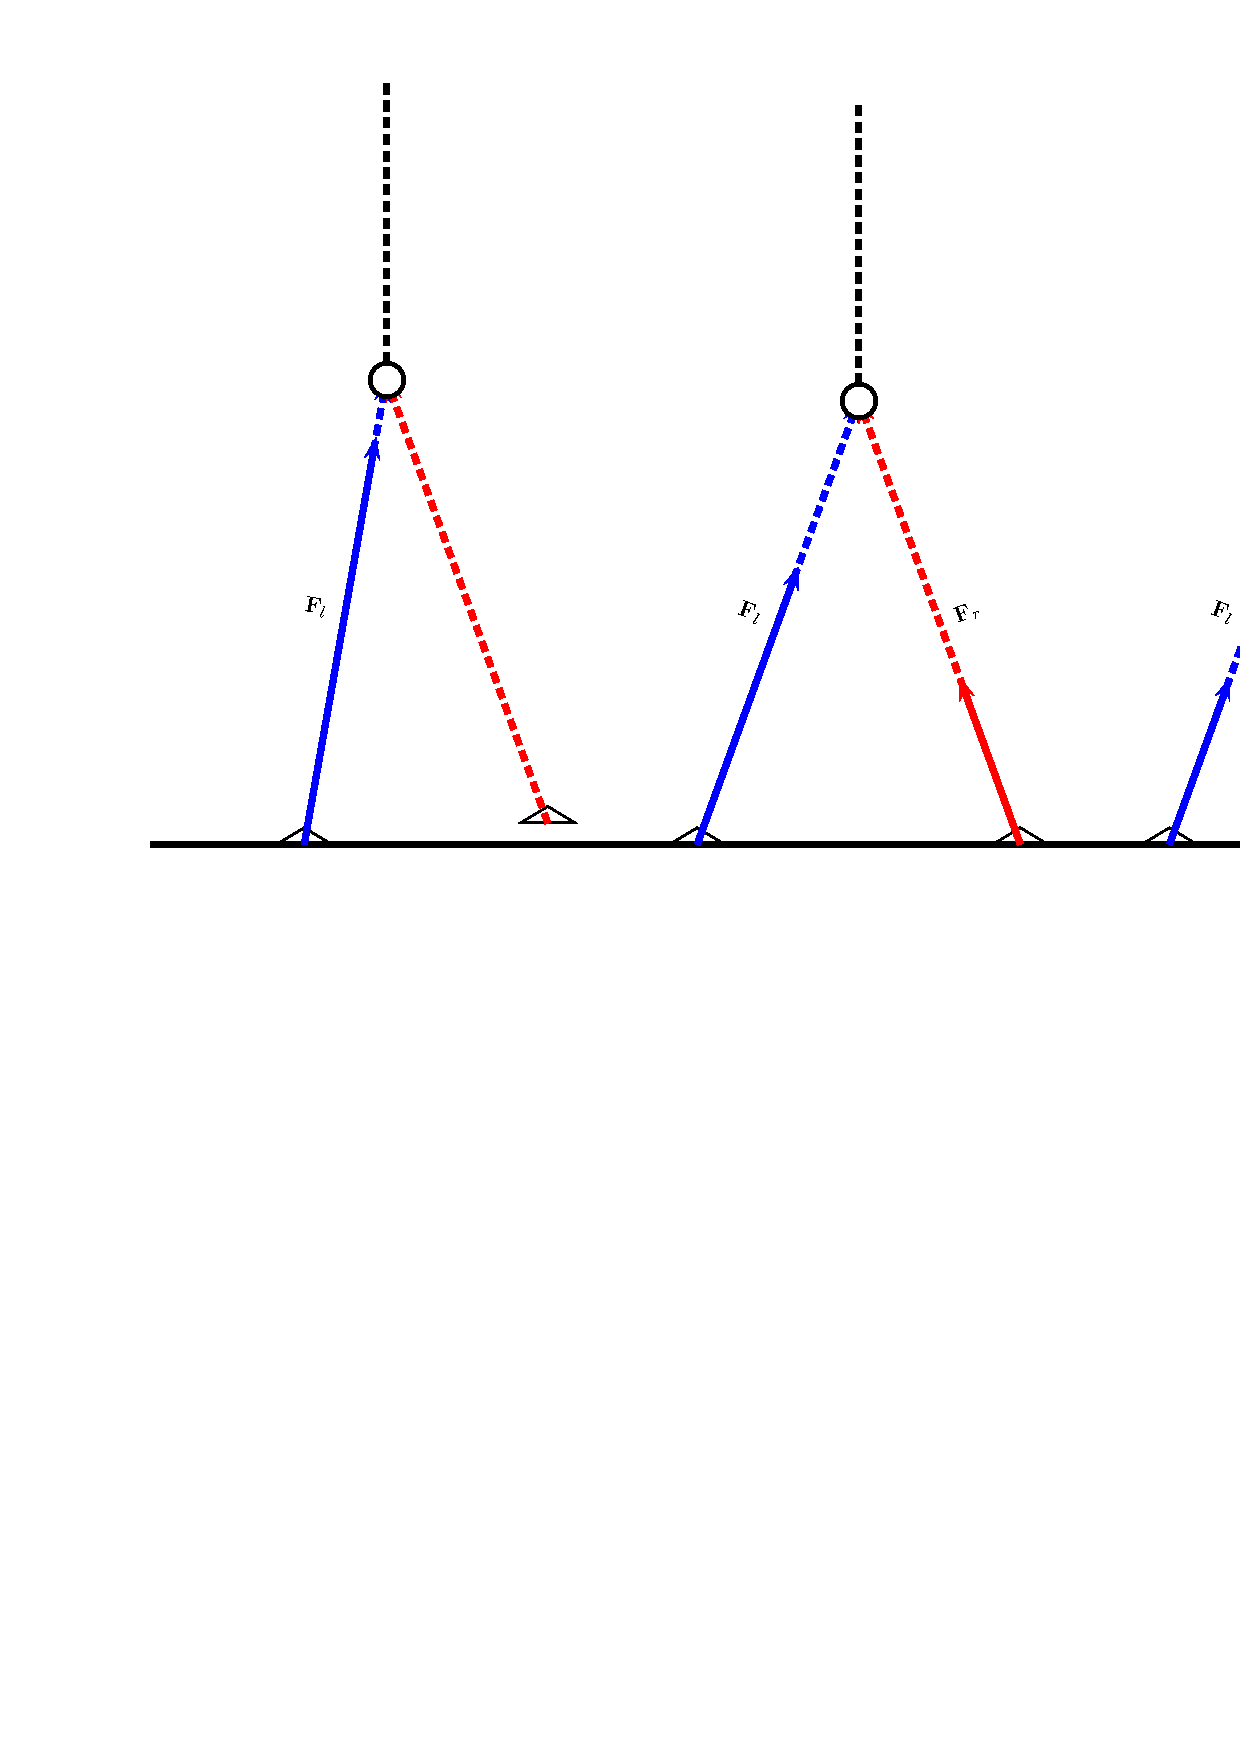
\includegraphics[height=6in]{stanceConfigure}
    \else
      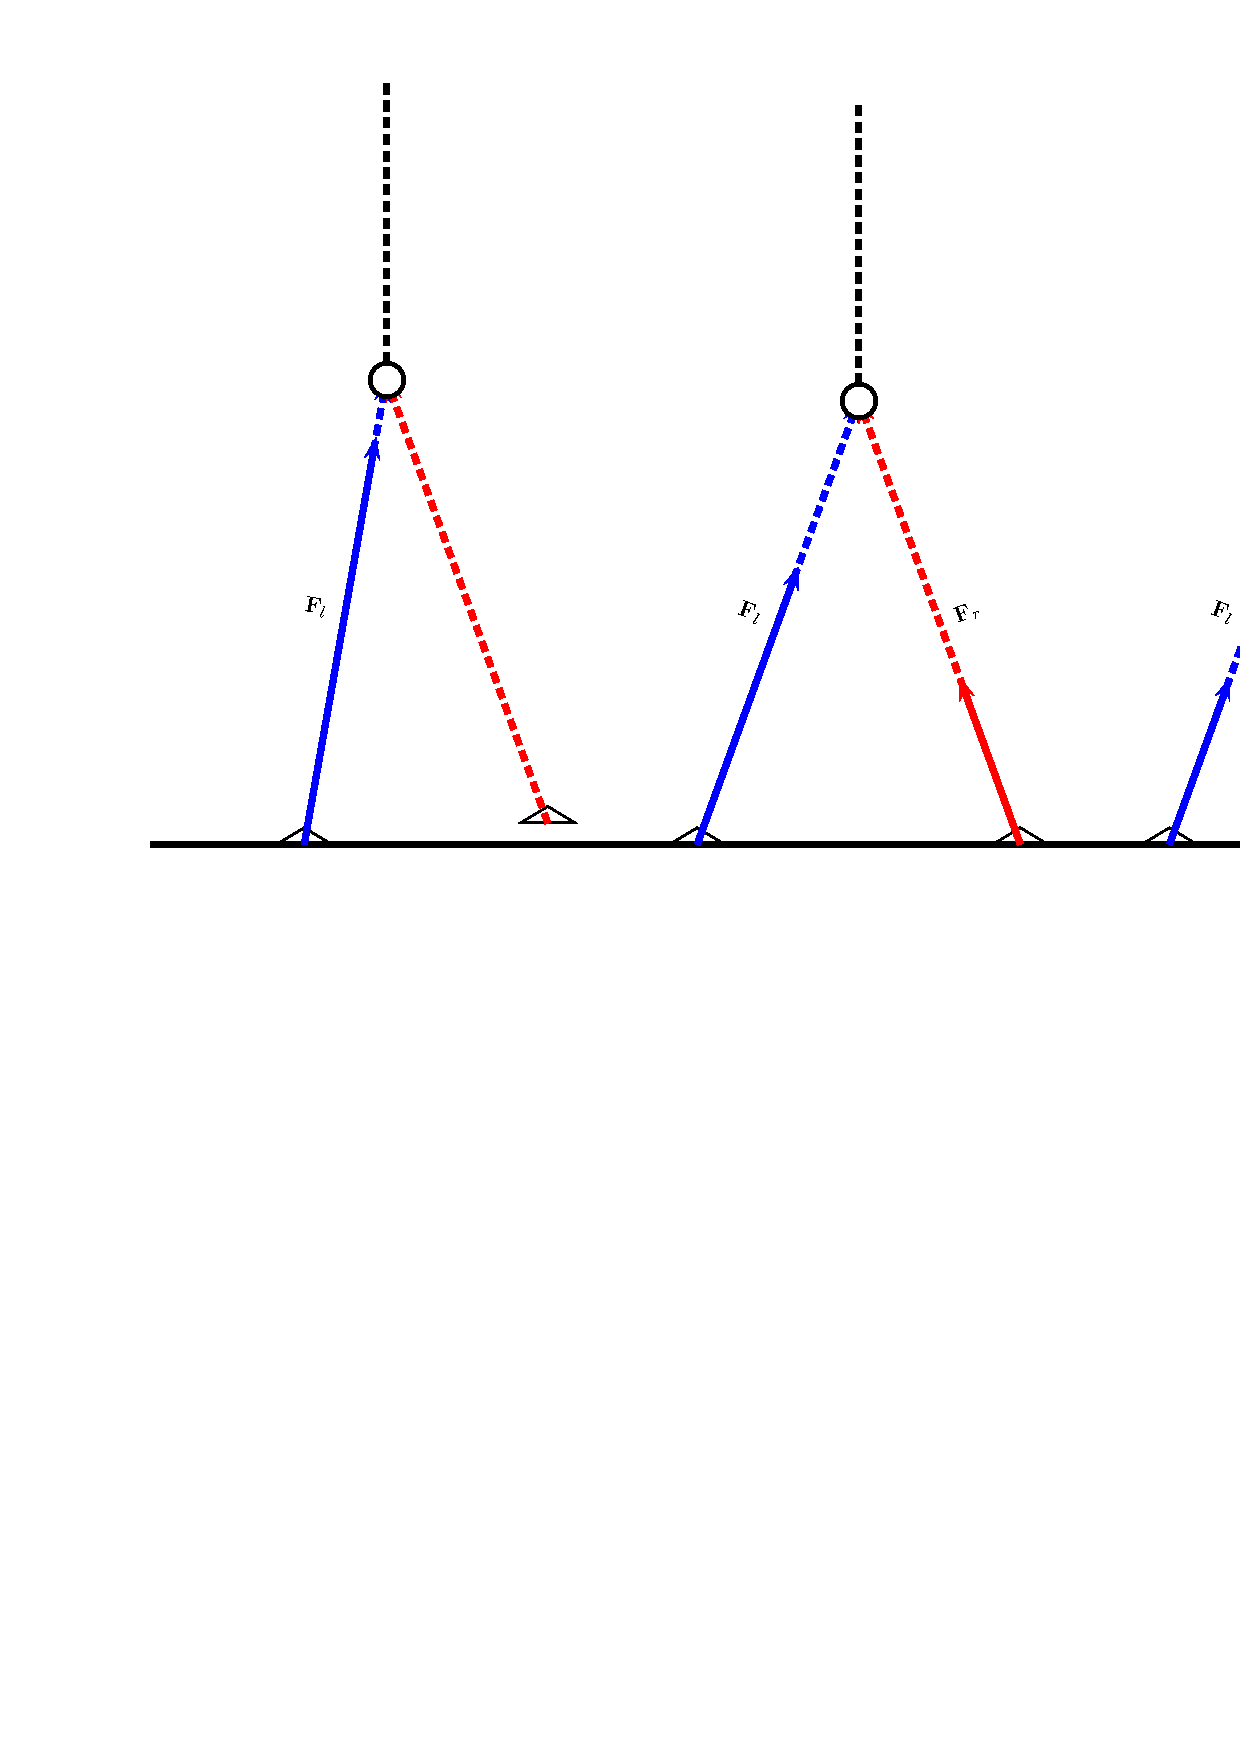
\includegraphics[width=0.7\textwidth]{stanceConfigure}
    \fi
    \caption{The Stance Motion Posture}
    \label{fig:stancepostures}
\end{center}
\end{figure}

the stance is easy for human, but the dynamic is not trifile.
stance is not continues system,the dynamic involves three phase

\begin{itemize}
\HiItem{Double Support}
When the horitontal displace model is small, people stand with two legs support.
the motion is governed by the gravity.
\[
\ddot{q}=\frac{g}{L}w_r(y_m-y_r)+\frac{g}{L}w_l(y_m-y_l)
\]


but usually some intutive strategy is applyied.
if the two legs generate torque to maintain the posture, the two torques should not be euqal,
if the center moving to the left, then the left torque will generate more torque.
if the center moving to the right, then the right leg will generate more torque.
supporse the realitionship is linear.
then we get the following intutive control stance equation, which we used as the mechanical oscillator.
\begin{equation}
\label{eq:stanceequation}
\ddot{q}=\frac{g}{L}w_r(y_m-y_r)+\frac{g}{L}w_l(y_m-y_l)+\frac{\tau_L+\tau_R}{mL}
\end{equation}



\HiItem{Single Leg Support}
if the there is a big horizontal displacement, there pepole will stand with single leg.
passively, the equaltion is 
\[
\ddot{q}=\frac{g}{L}q
\]
and intutive even controlled
\begin{equation}
\label{equ:singlestand}
\ddot{q}=\frac{g}{L}q+\frac{y_{L,R}}{L}\tau_{L,R}
\end{equation}

\HiItem{Fall and Walk}
if the displacement is even bigger,then the walker will move out the support region.
for a human, where the stance region is depends on the  hight and the stepsize.
And the goal of balancing is to maintain the system state within the support region.

usually,it will result two motion sequence, wheather it will start to walk for it will fall


\end{itemize}

\section {Stance Control}
\subsection{Entraintment}

without damping effects,the original system is simmilar to mass spring system.
It wil vibrate continutelly.

the phase plot is shown in
\begin{figure}[!htbp]
  \begin{center}
    \leavevmode
    \ifpdf
      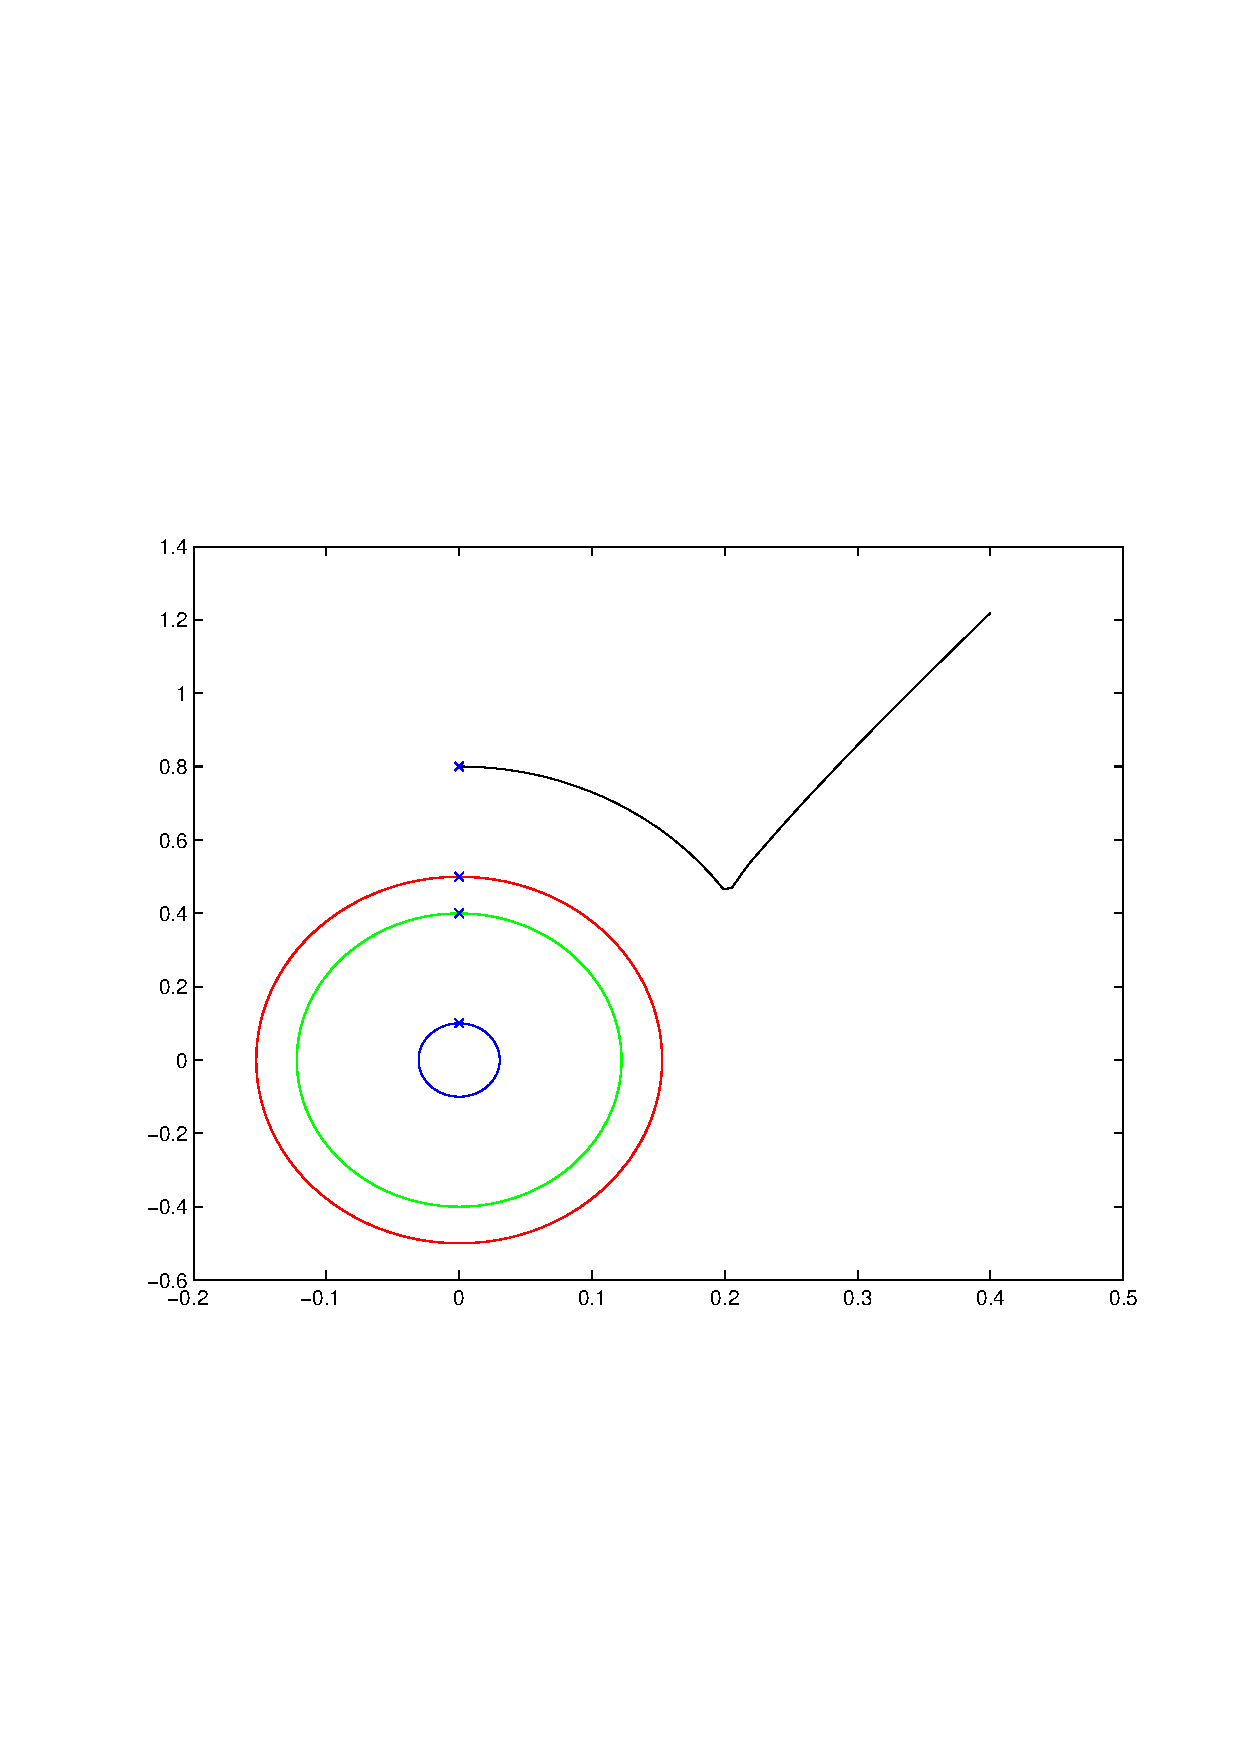
\includegraphics[height=6in]{uncontrolled}
    \else
      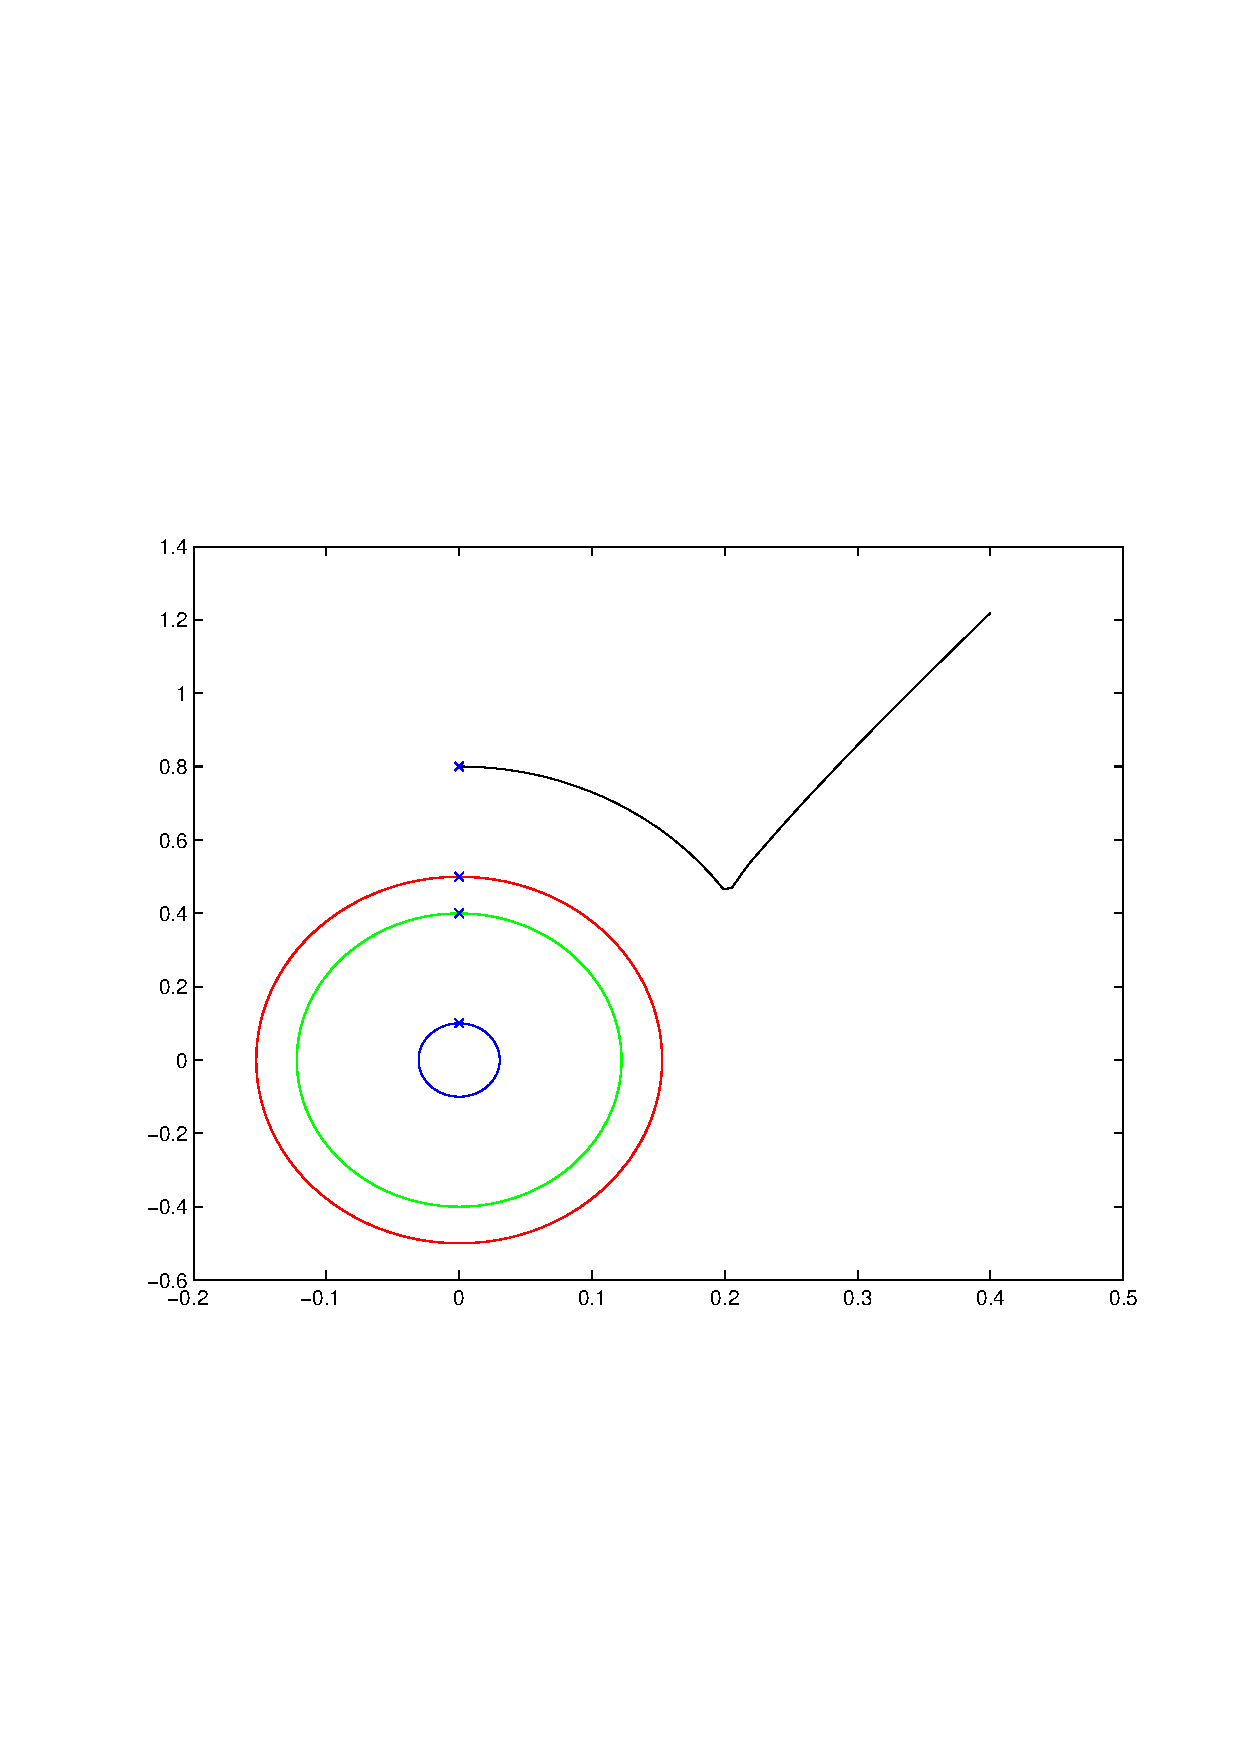
\includegraphics[width=0.7\textwidth]{uncontrolled}
    \fi
    \caption{un controlled motion}
    \label{fig:stancepostures}
\end{center}
\end{figure}

if the the initial speed is higher, then it will move out the support region.



while in our method ,by coubling neural system the the oscillator, it will form a limit circle,
but for this situation of standing, limit circle doesn't not boost the stablity,because the boundary is fixed,
neural oscillator will not modify the boudary,and it is impossible for mechanical system to converge to the limit circle within 1/4 period.
thus we make the output of the output of neural controller very small $\uout$.

Limit Circle is useful for it can make stance start to vibrate at a constant speed, this will be very helpful when we start from stance to walk.

\subsection{Local Invariant Control}
All the three group controller can be used,but basically only two control method are useful.
\subsubsection*{Time Scaling}
The first is time scalling $G_ts$
as show in figure
\begin{figure}[!htbp]
  \begin{center}
    \leavevmode
    \ifpdf
      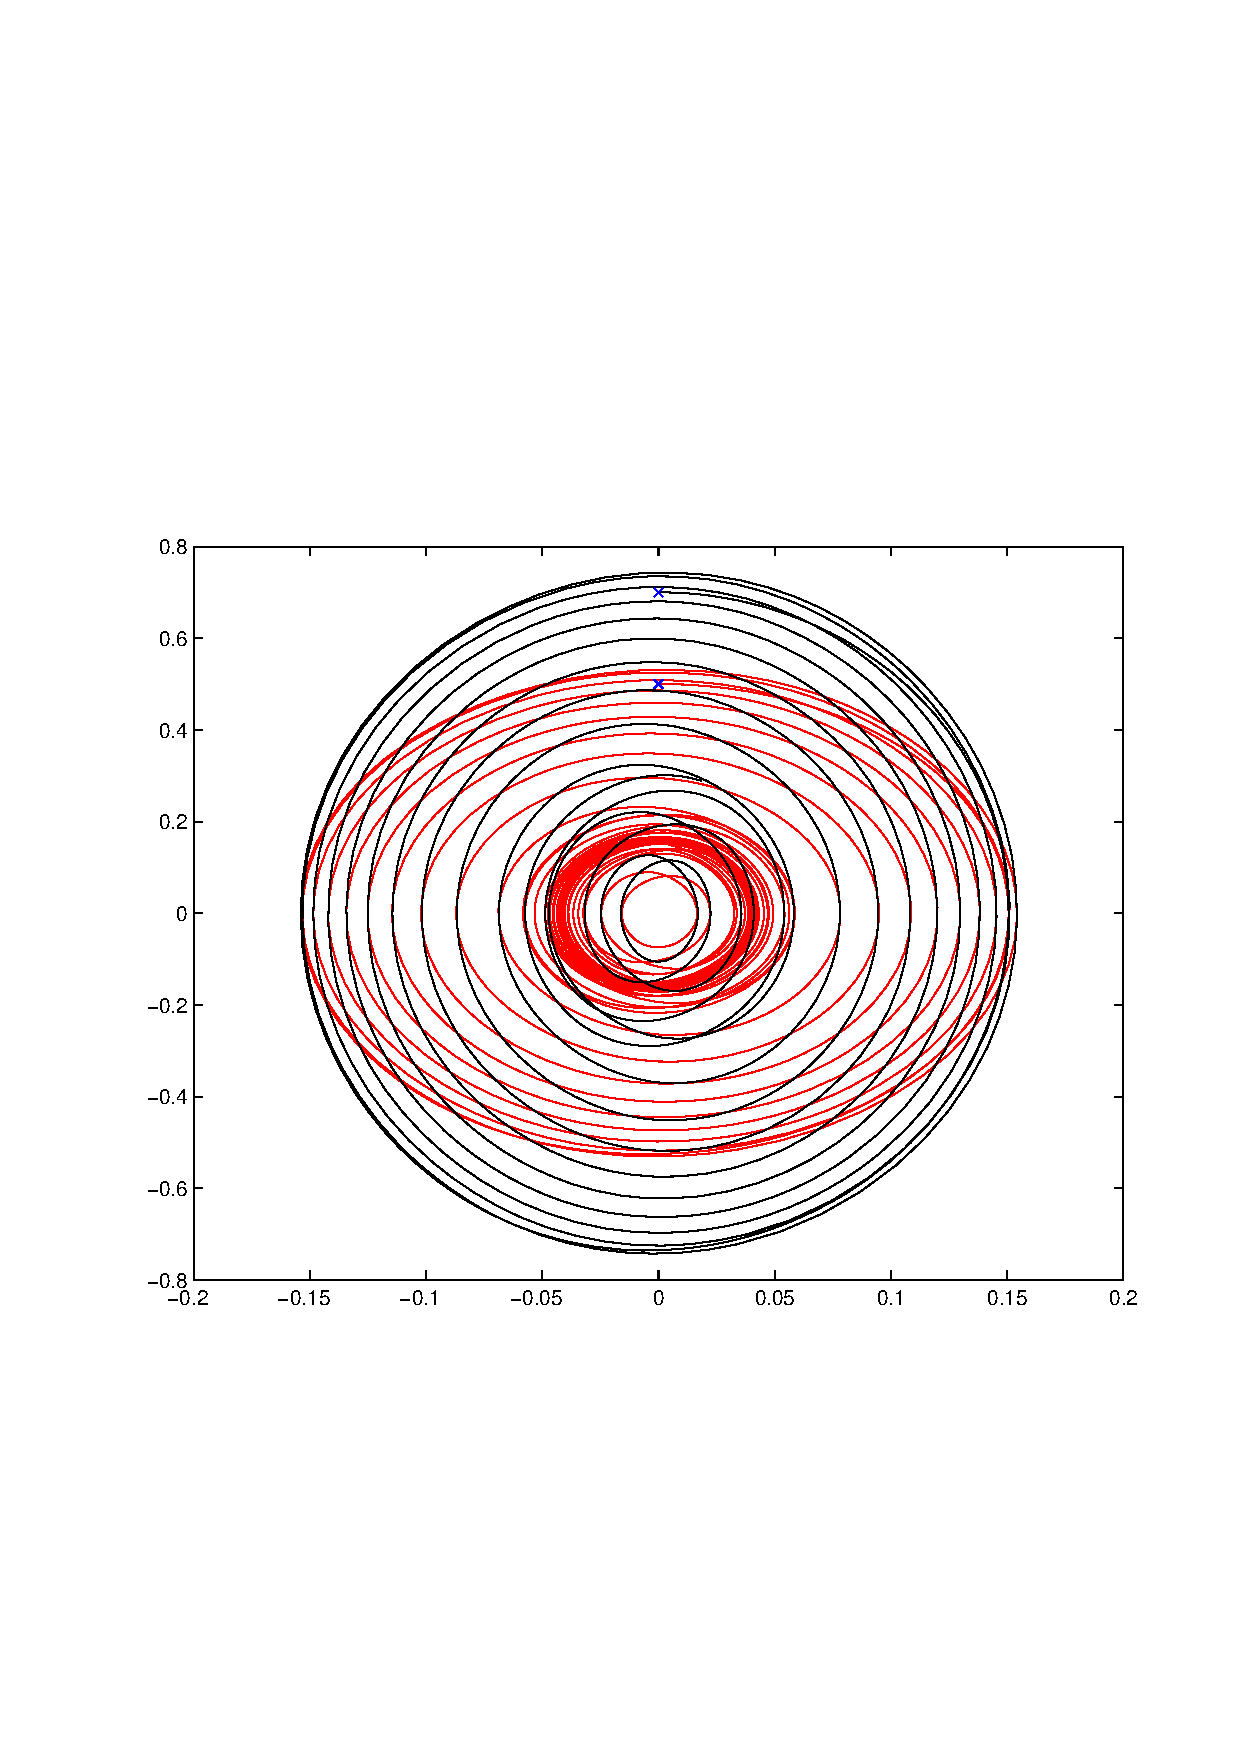
\includegraphics[height=6in]{TimeScaling}
    \else
      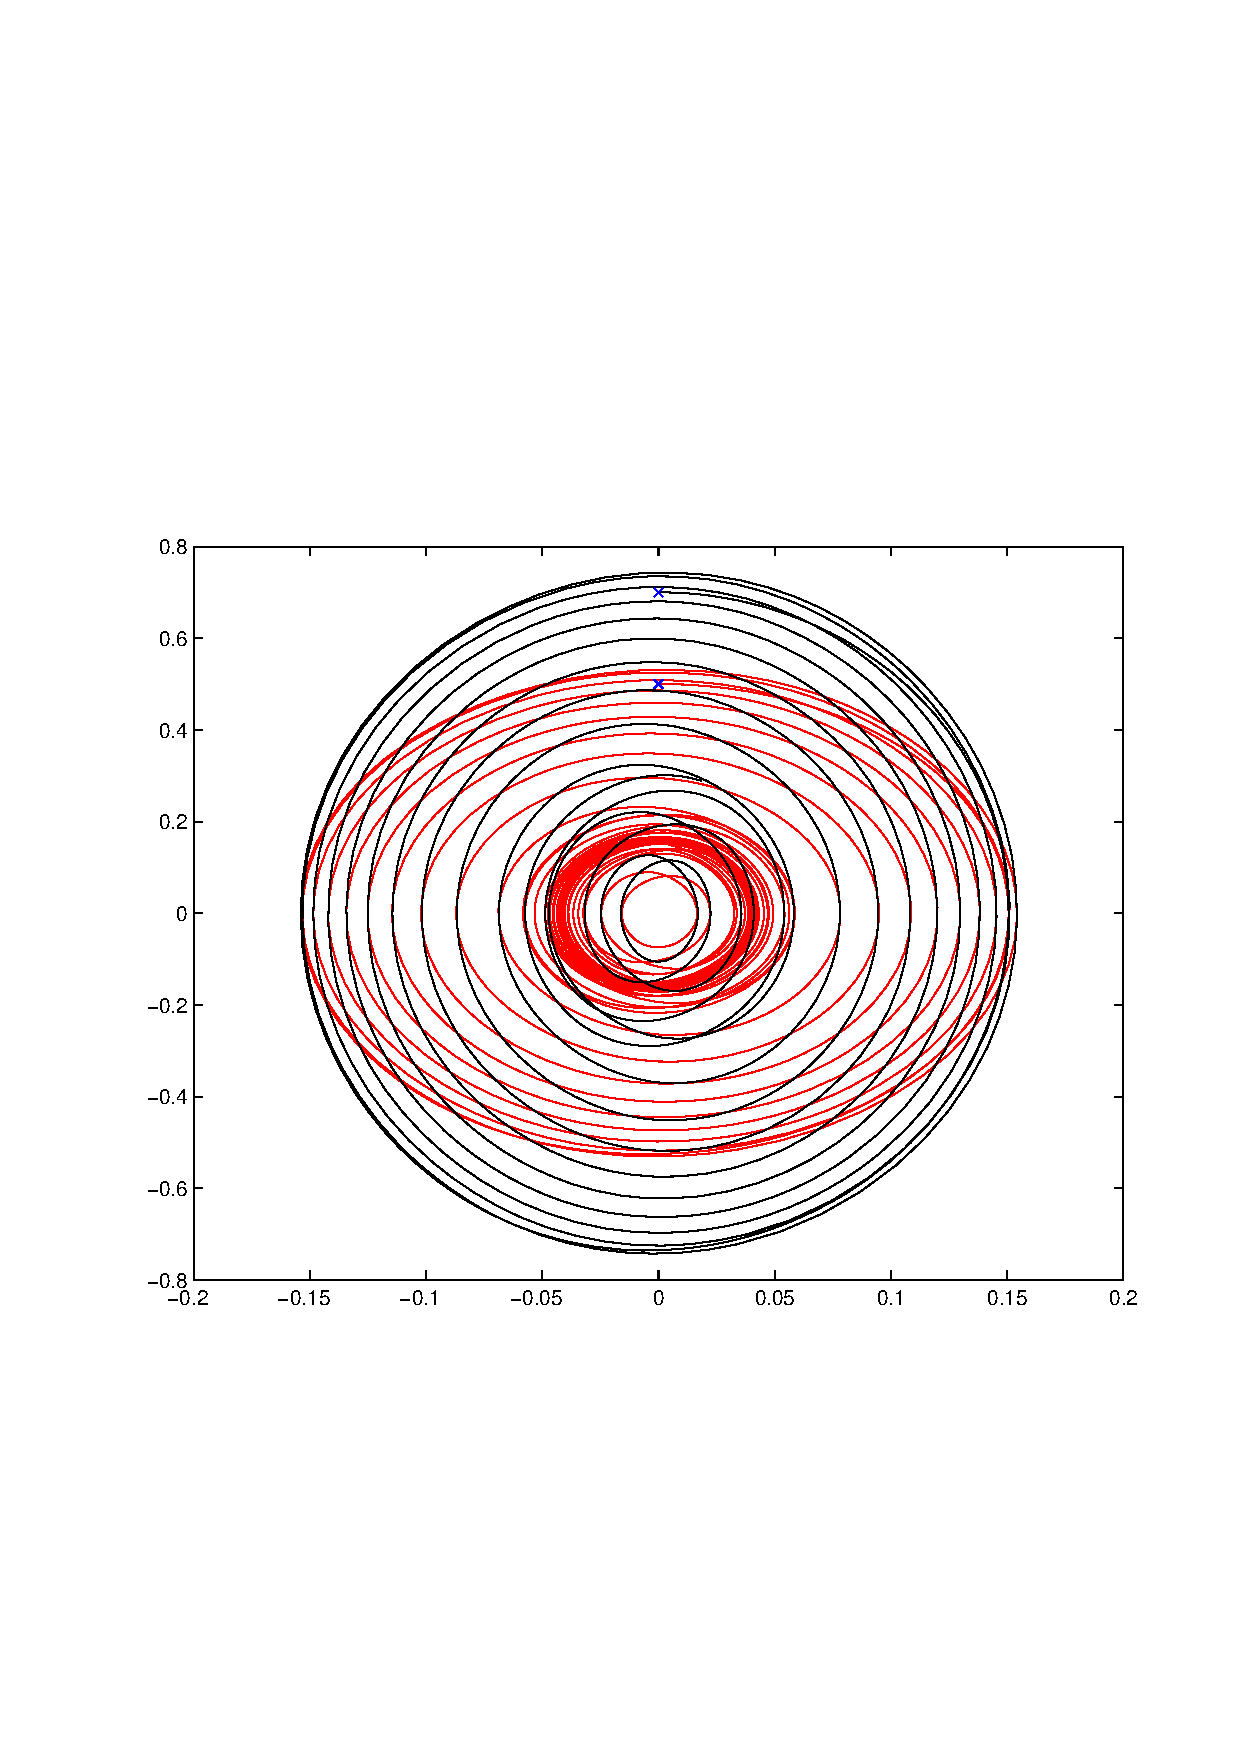
\includegraphics[width=0.7\textwidth]{TimeScaling}
    \fi
    \caption{Time Scaling}
    \label{fig:stanceTimeScaling}
\end{center}
\end{figure}

The falling motio is show in the figure ~\ref{fig:stancefall}
\begin{figure}[!htbp]
  \begin{center}
    \leavevmode
    \ifpdf
      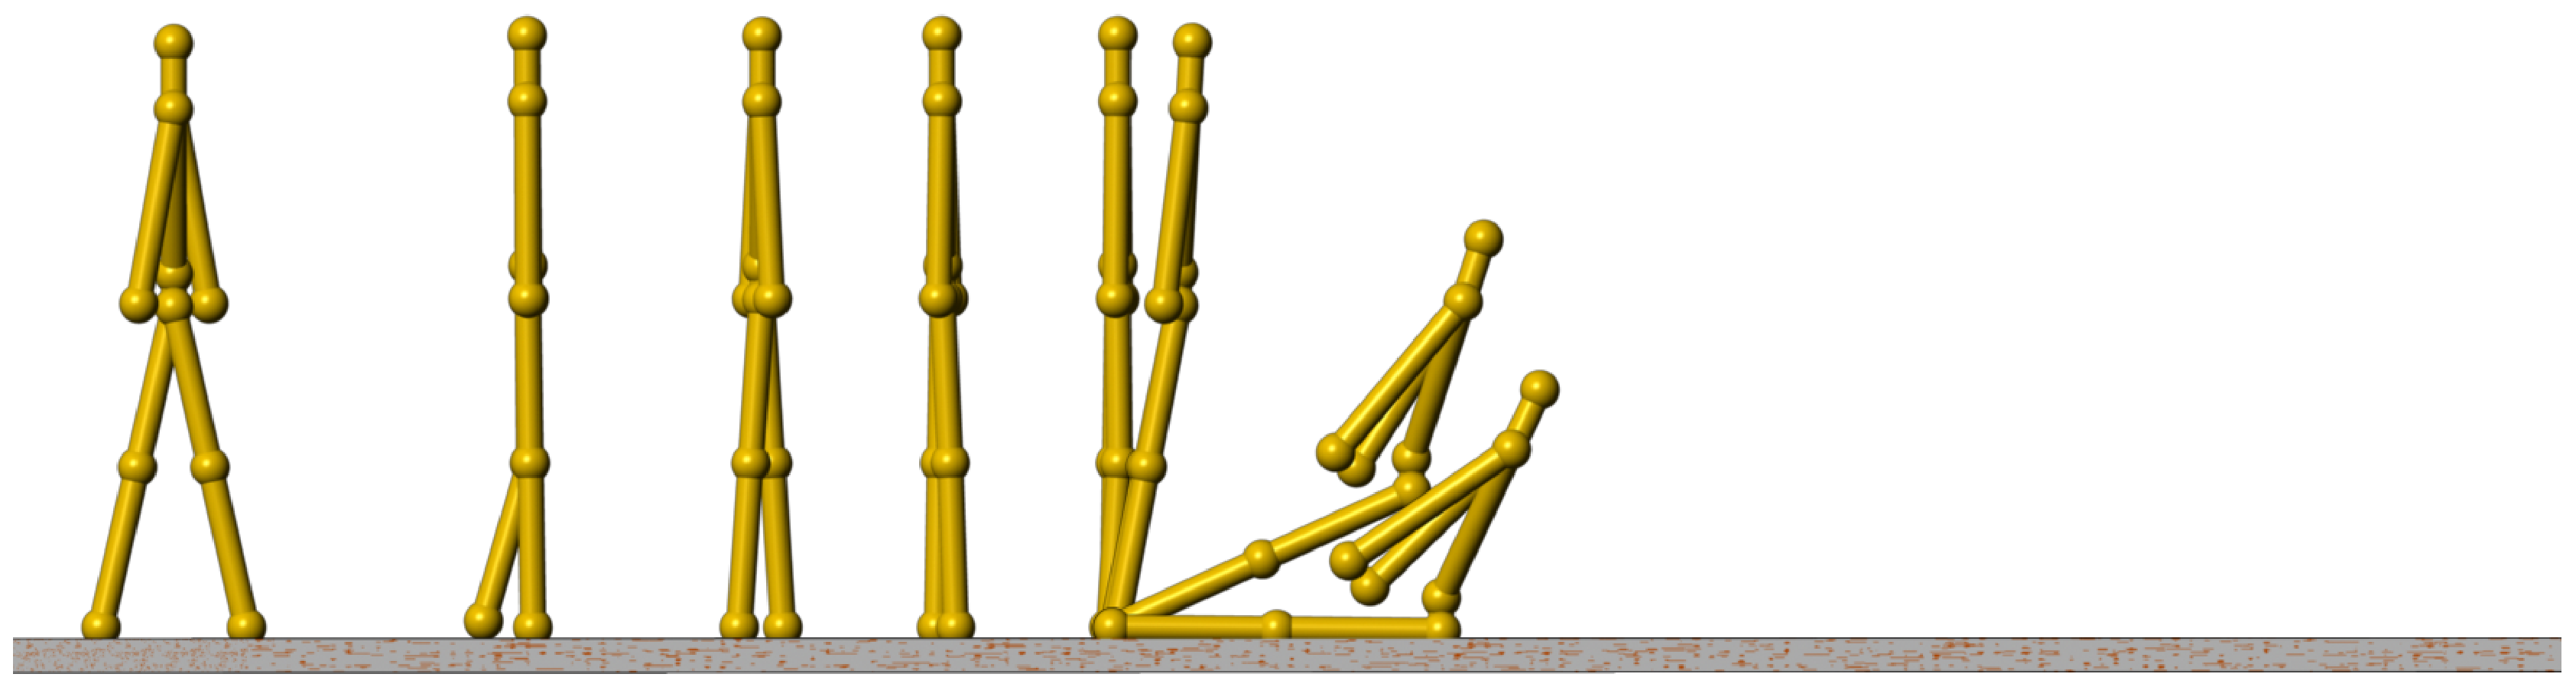
\includegraphics[height=6in]{PlaceHolder}
    \else
      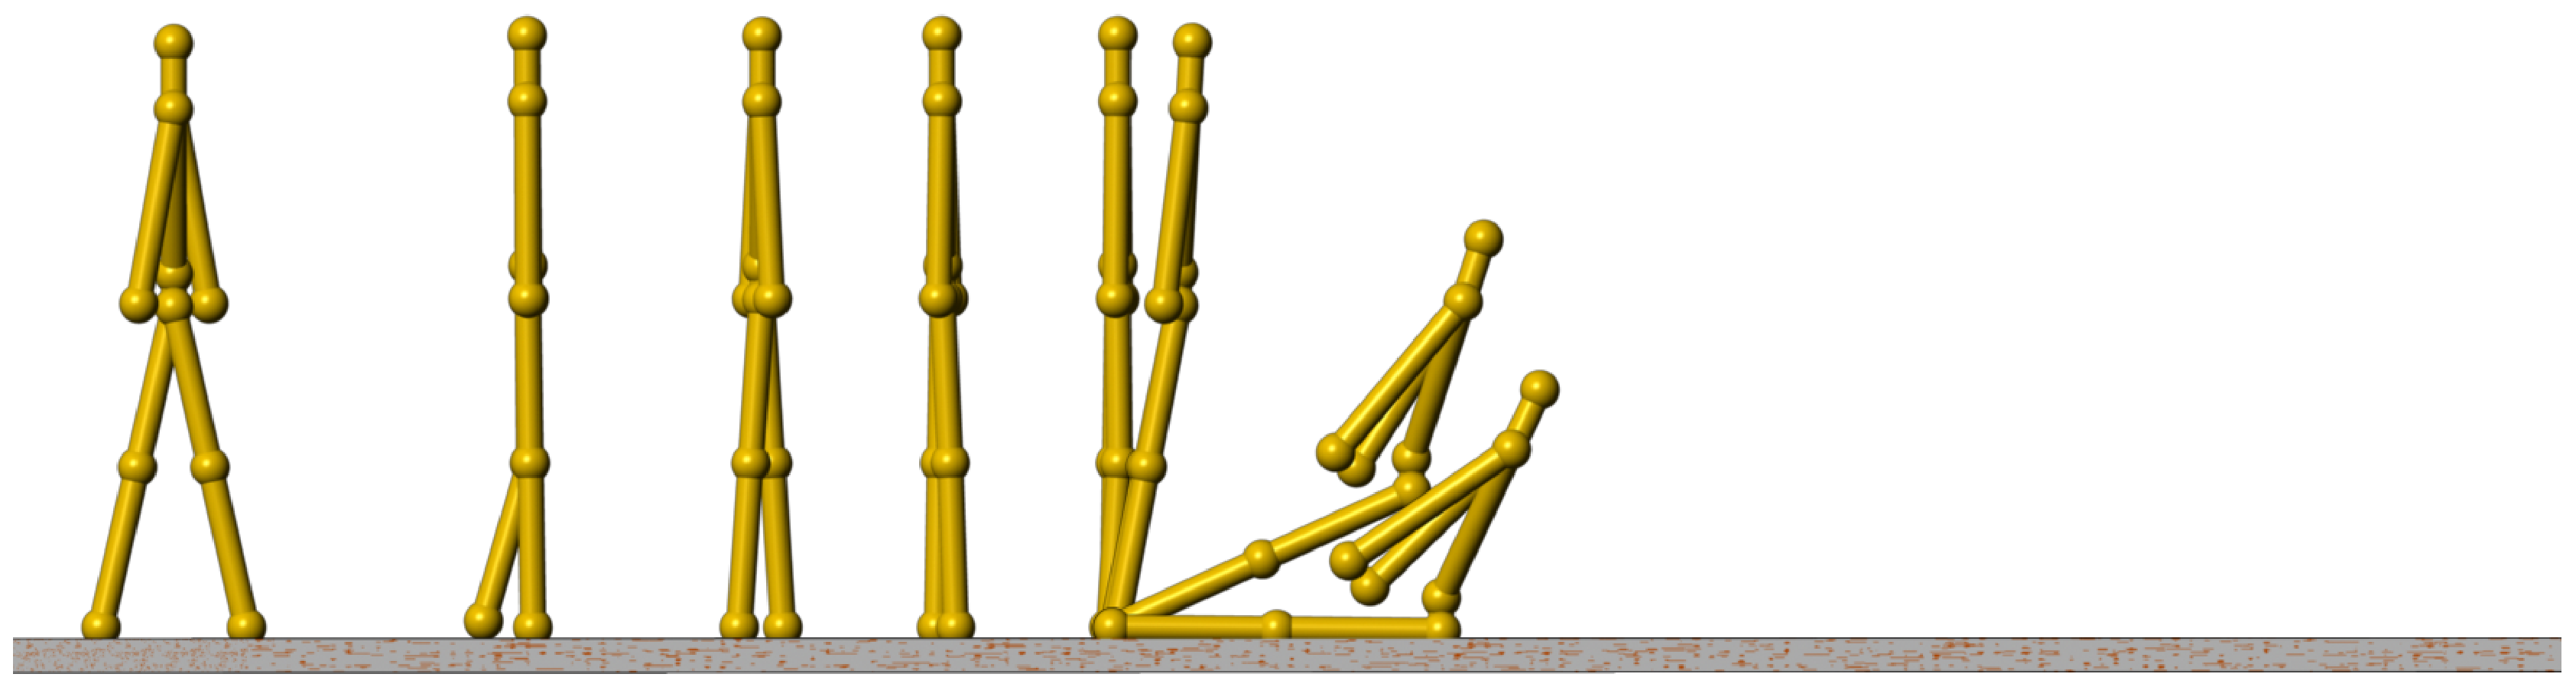
\includegraphics[width=0.7\textwidth]{PlaceHolder}
    \fi
    \caption{Place Holder}
    \label{fig:stancefall}
\end{center}
\end{figure}

\subsubsection*{Energy Control}
By modifying the Energy Scalling, we can modify the size of limit circle, the will adjust the oscillation amplitude.
as show in Figure~\ref{energyscaling}
\begin{figure}[!htbp]
  \begin{center}
    \leavevmode
    \ifpdf
      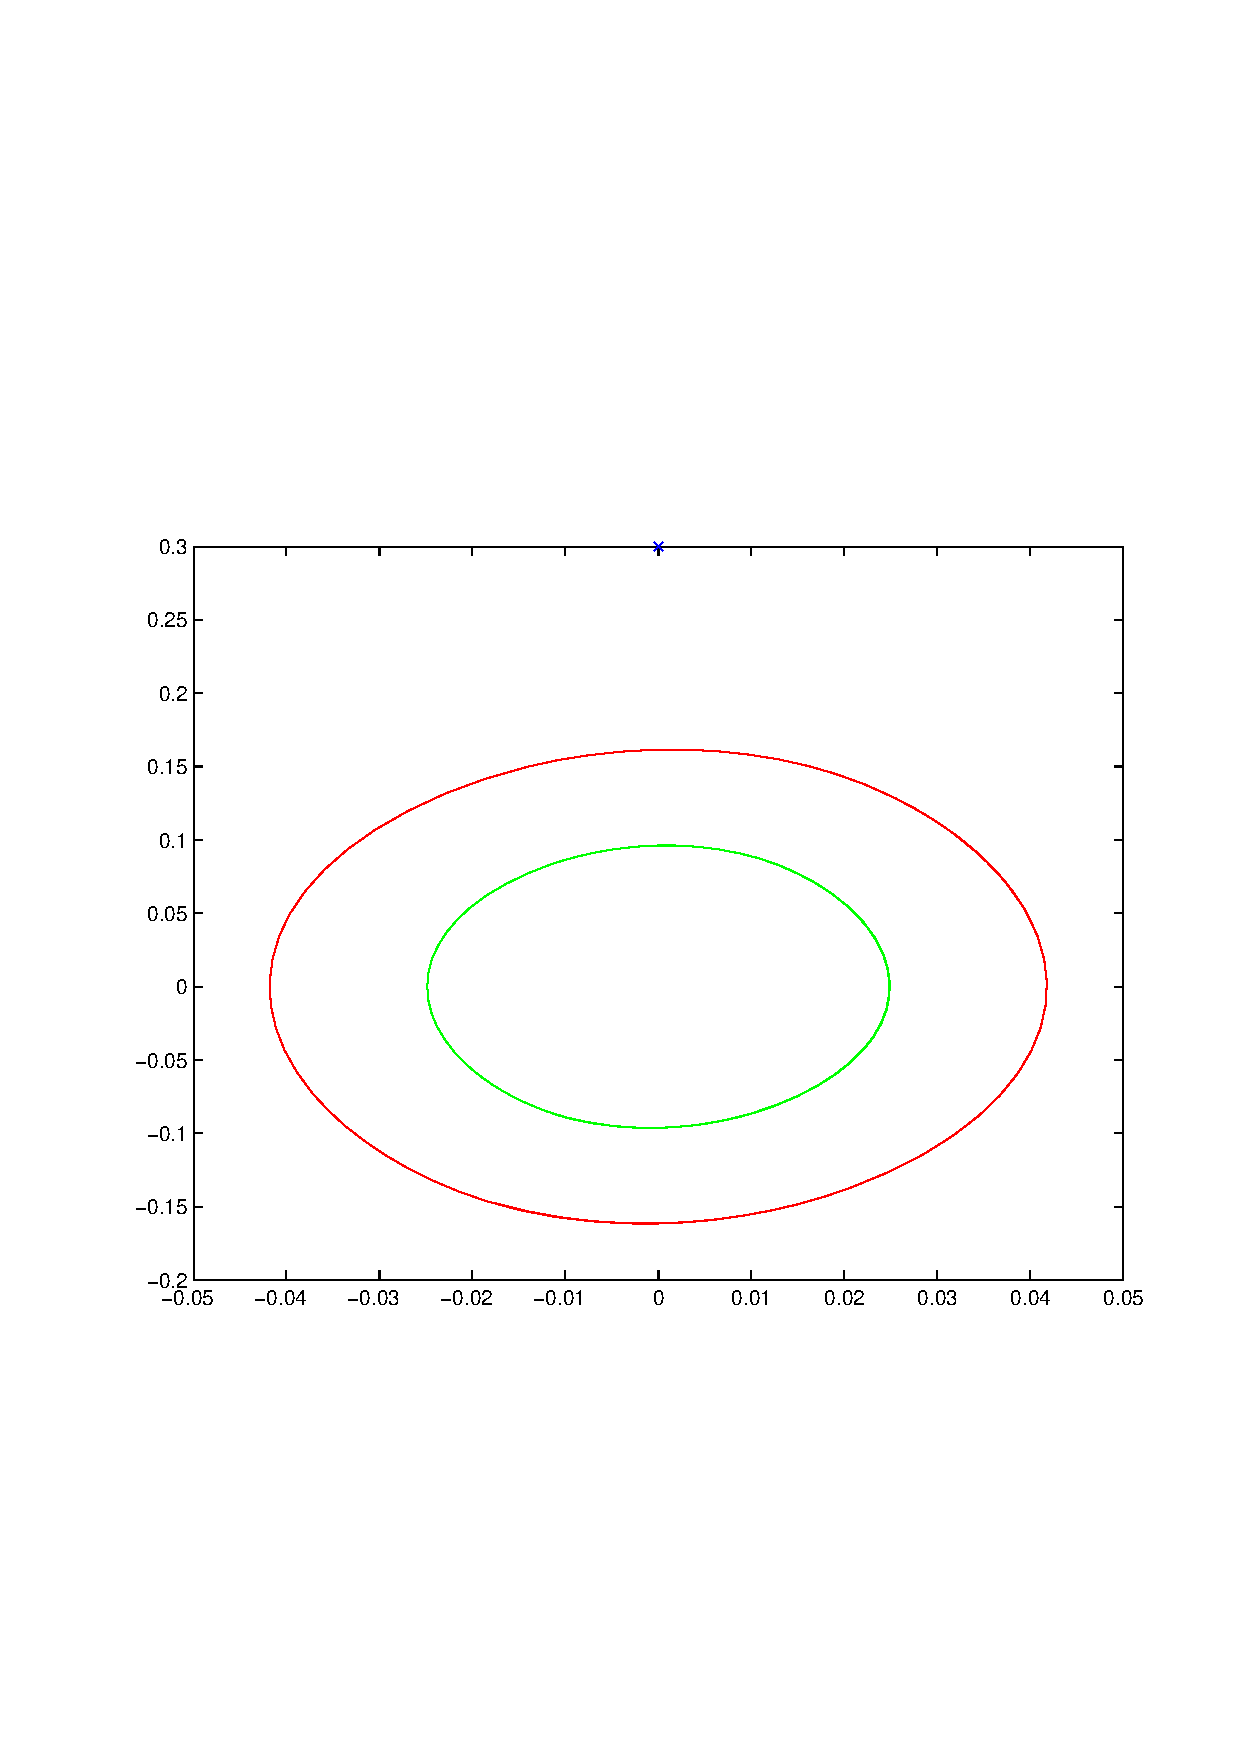
\includegraphics[height=6in]{EnergyControlled}
    \else
      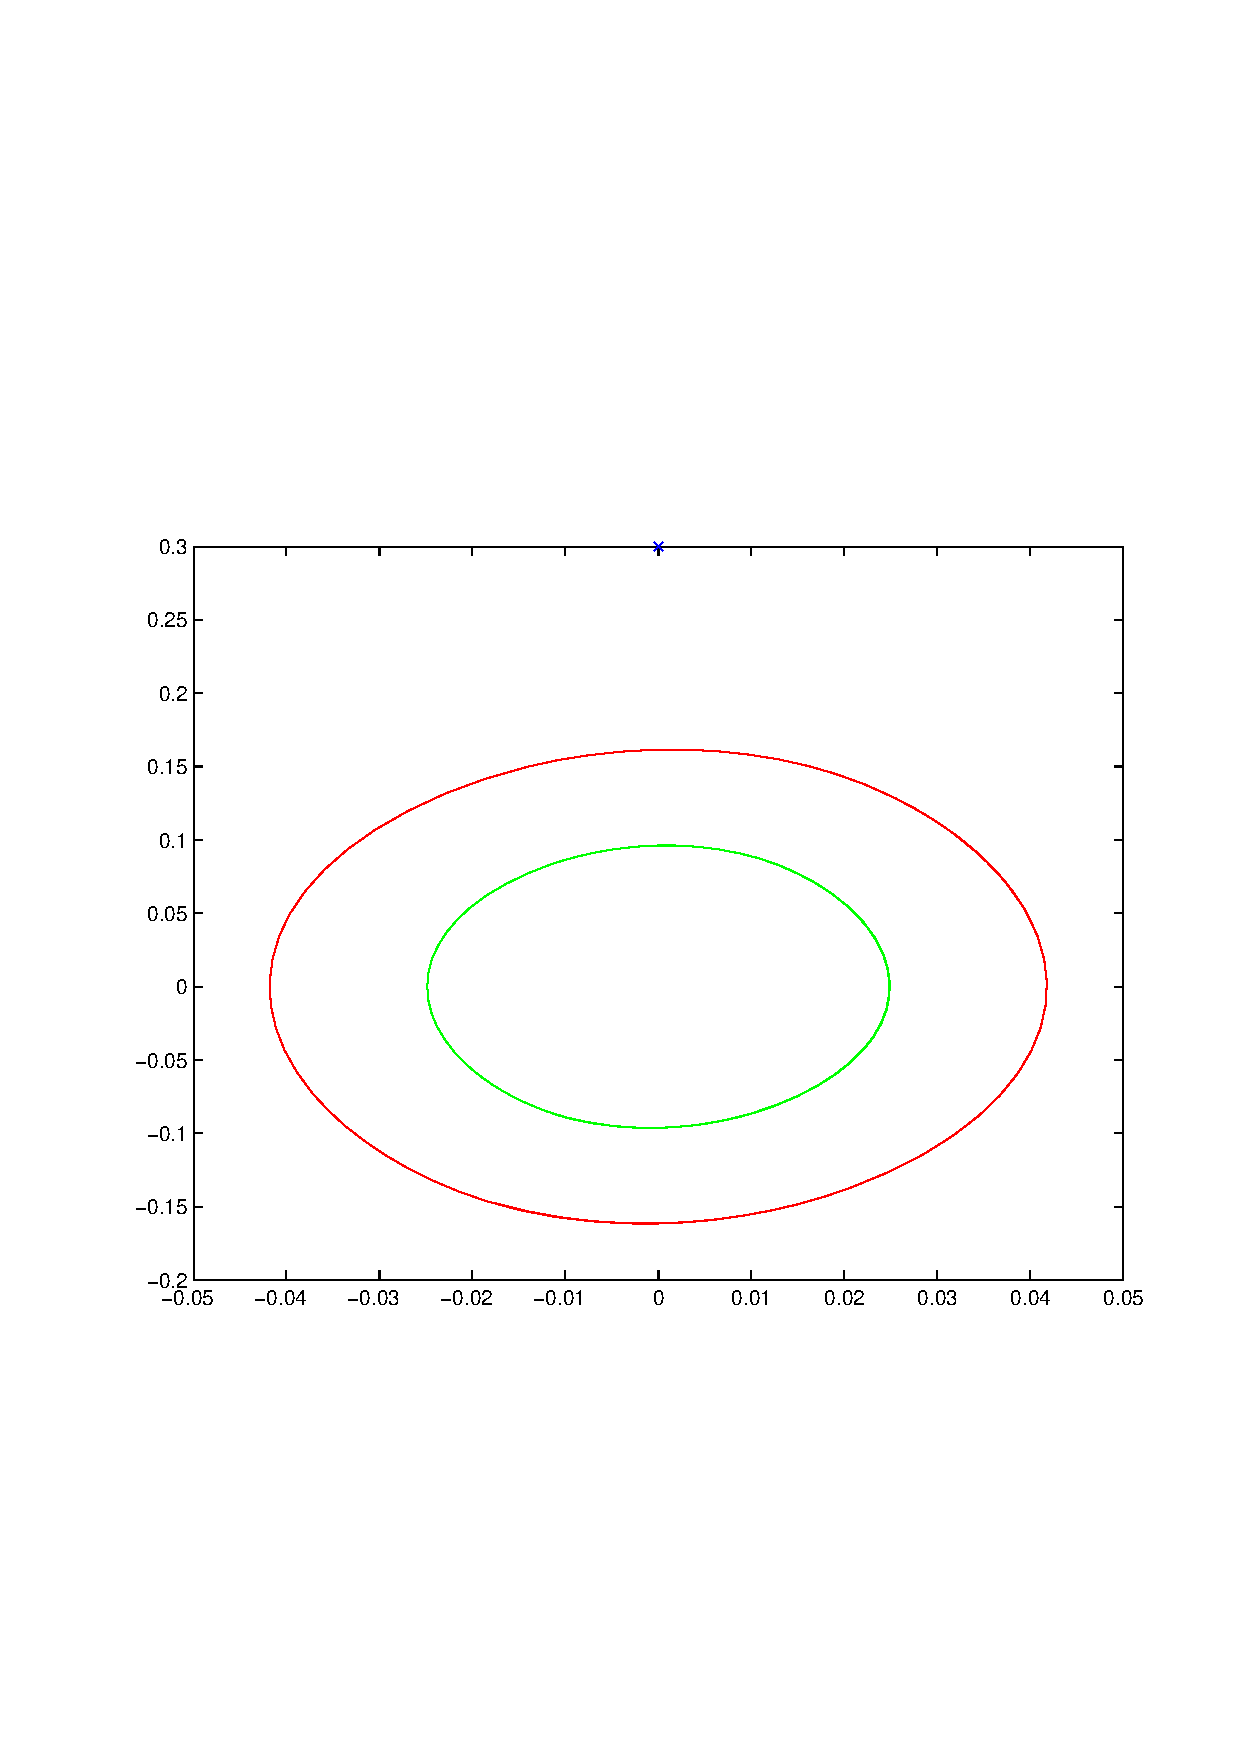
\includegraphics[width=0.7\textwidth]{EnergyControlled}
    \fi
    \caption{Energy Scaling}
    \label{fig:energyscaling}
\end{center}
\end{figure}


but it will also shrink the size of basin of attraction.




\subsubsection*{Fast Stable}
by applying speed and energy scalling sequecely, we can make the stance pos coverge in a quick speed.
as shown in figure ~\ref{fig:fastconverg}
\begin{figure}[!htbp]
  \begin{center}
    \leavevmode
    \ifpdf
      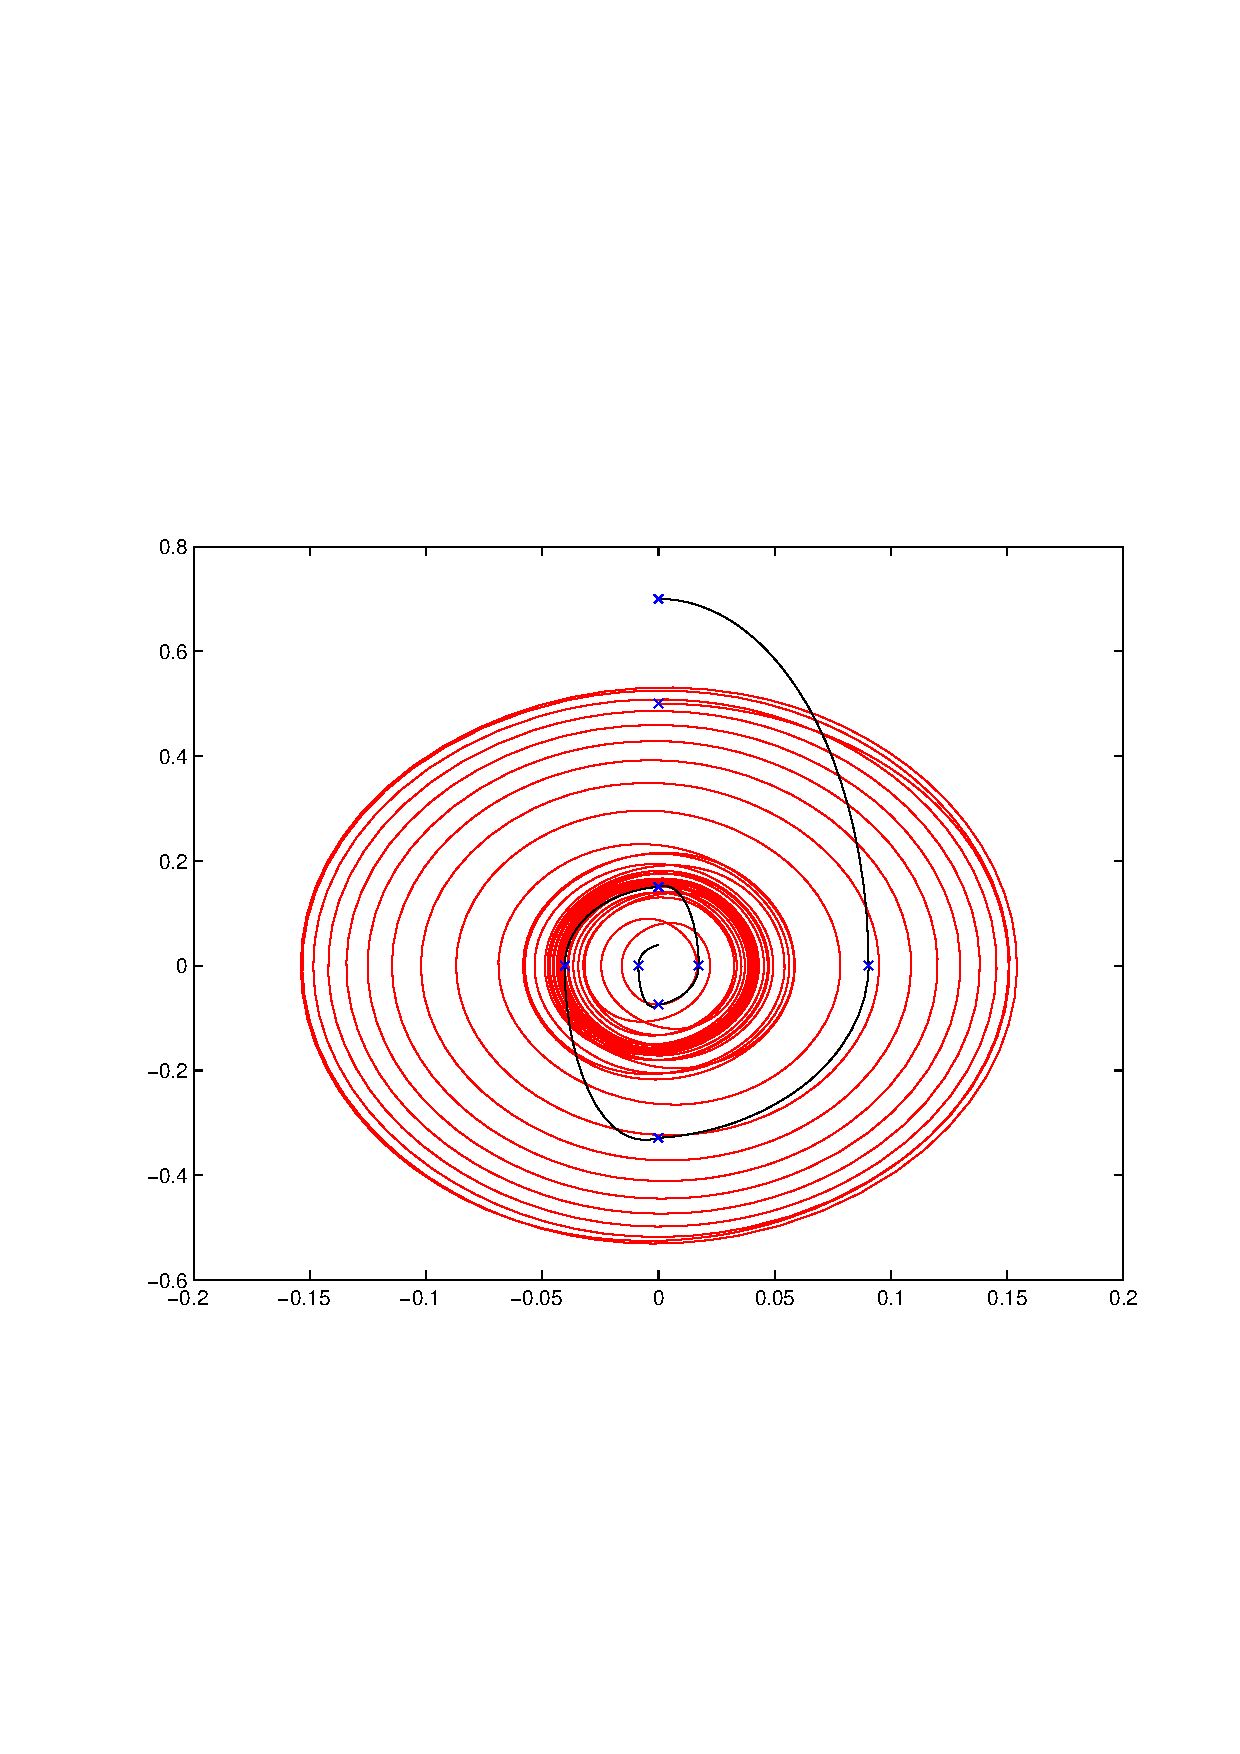
\includegraphics[height=6in]{FastCoverge}
    \else
      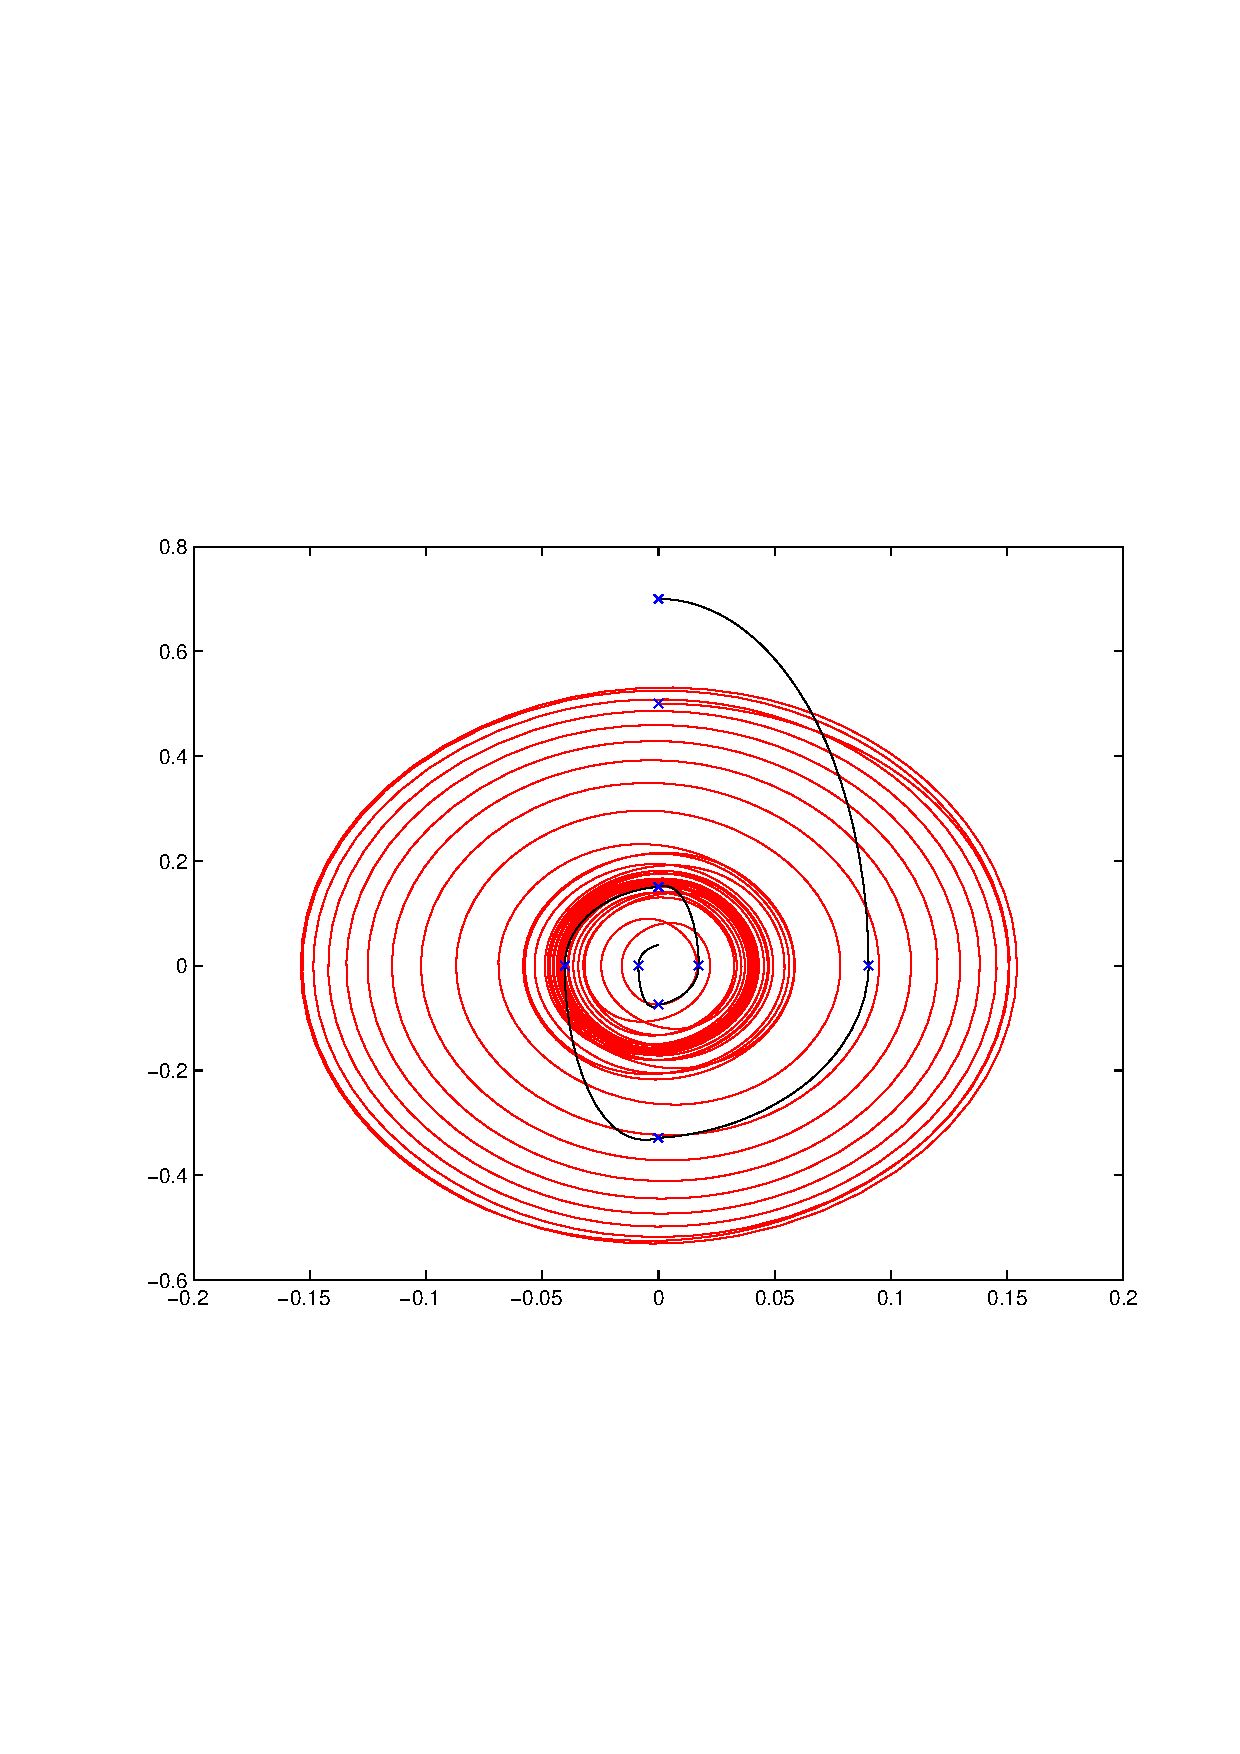
\includegraphics[width=0.7\textwidth]{FastCoverge}
    \fi
    \caption{Fast Converge}
    \label{fig:fastconverg}
\end{center}
\end{figure}


\section{Walking and Stance Transition}



we phase plot we show the limit circle of two motion primitives.

\begin{figure}[!htbp]
  \begin{center}
    \leavevmode
    \ifpdf
      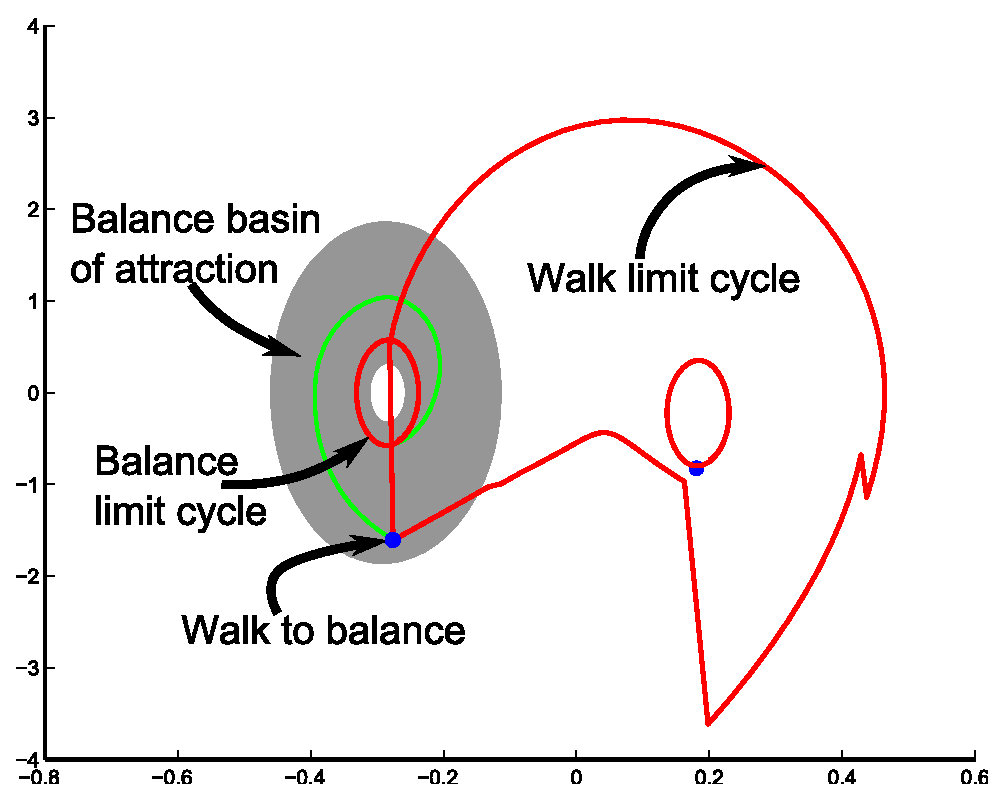
\includegraphics[height=6in]{walk_to_stand}
    \else
      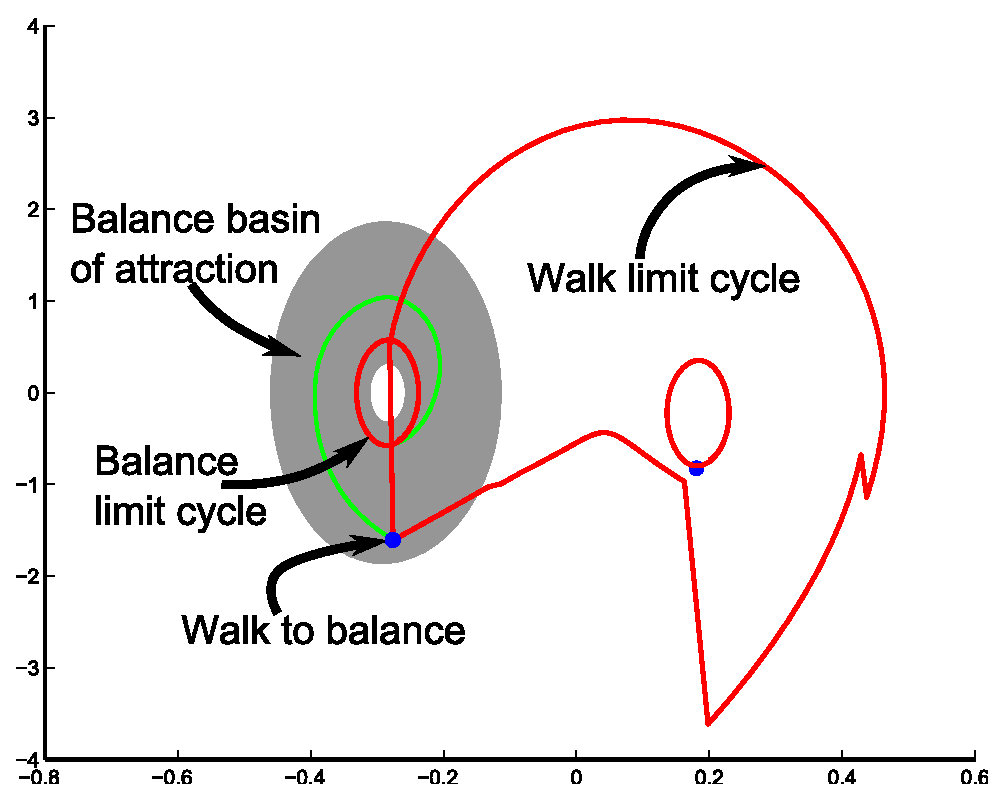
\includegraphics[width=0.7\textwidth]{walk_to_stand}
    \fi
    \caption{Fast Converge}
    \label{fig:fastconverg}
\end{center}
\end{figure}

the phase plot here shows the supporting leg, the swing leg is show in shadow red


\subsection{Walk to Stance}
walk to stance transition happens at the heel strike phase.
if without control effort, the bipedal machine will continue two walk, while if we swich the on the stance controller,
the bipedal machine will converge to a small amplitue,then both legs start oscillation, this is the stance to walk.

we show in picture
\begin{figure}[!htbp]
  \begin{center}
    \leavevmode
    \ifpdf
      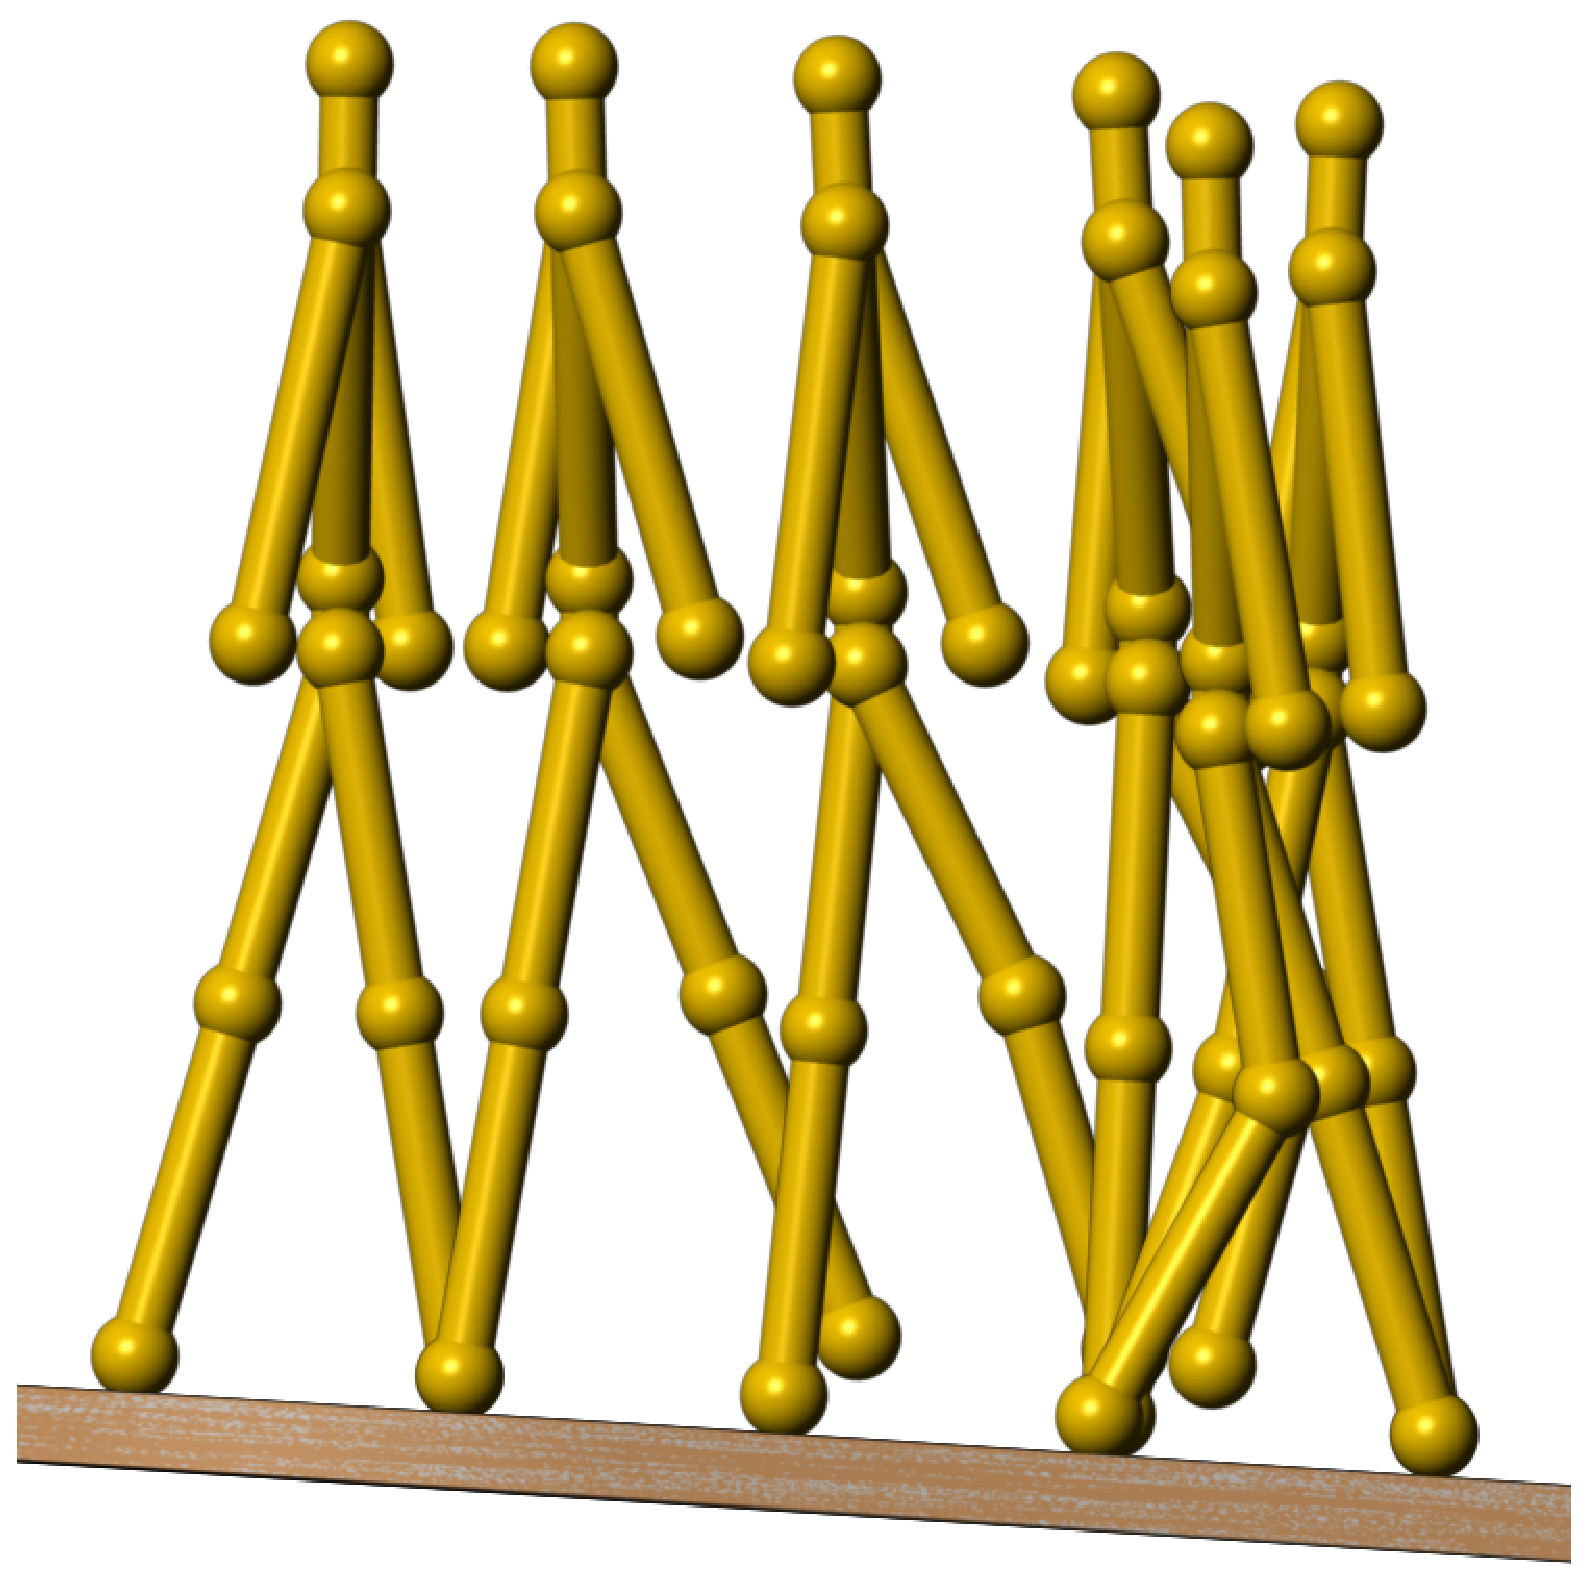
\includegraphics[height=6in]{walk_to_balance}
    \else
      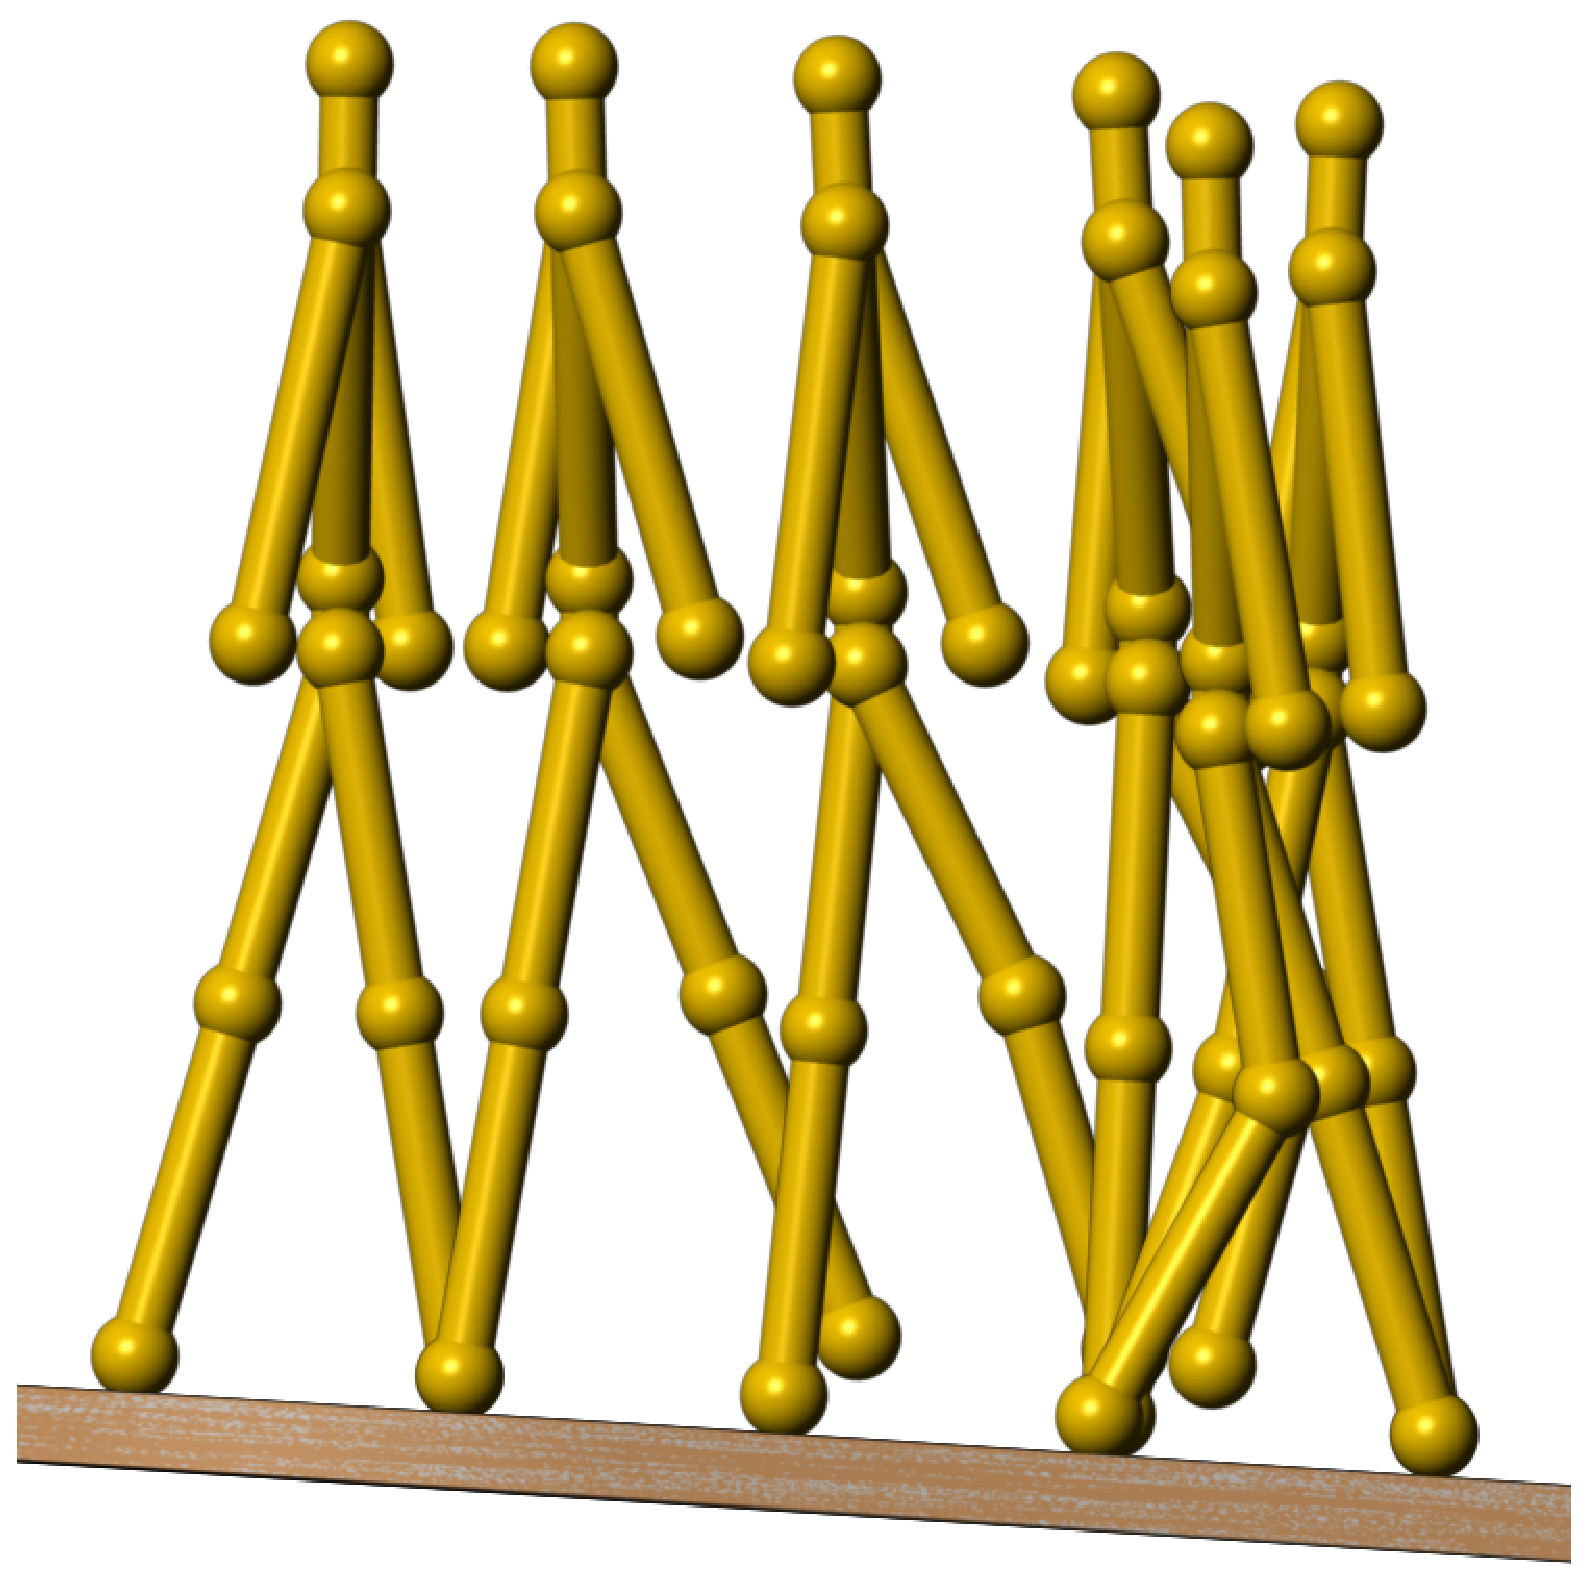
\includegraphics[width=0.7\textwidth]{walk_to_balance}
    \fi
    \caption{Walk to Balance}
    \label{fig:walk to balance}
\end{center}
\end{figure}

When walk to stance happens, the walker have to the stance controller must include the heel strike position.


\subsubsection*{Knee Bending Scheme}
When from walk to stance, that the heel strike time, the two legs are straight, for this case, the support region is very small.
Any push of the figure, it will move out of the two support region.
the walkers have to bend legs and lower the height.
Many possible ways can be develop for bending to lower the body height
We have develop many bending scheme, have seen many possible usage of the bending

\begin{itemize}
	\HiItem{One Leg Bending}
		walker can bend one leg while keep the other leg straght.
	\HiItem{Double Leg Bending}
		We can make the two leg bend.
\end{itemize}

it is very difficult to tell which one more realistic for human, basically, for when human walk, the knees is not necessary straight.
two two scheme provide is the exeme condition.

we have walking stance transition is shown in the following figures

\begin{figure}[!htbp]
  \begin{center}
    \leavevmode
    \ifpdf
      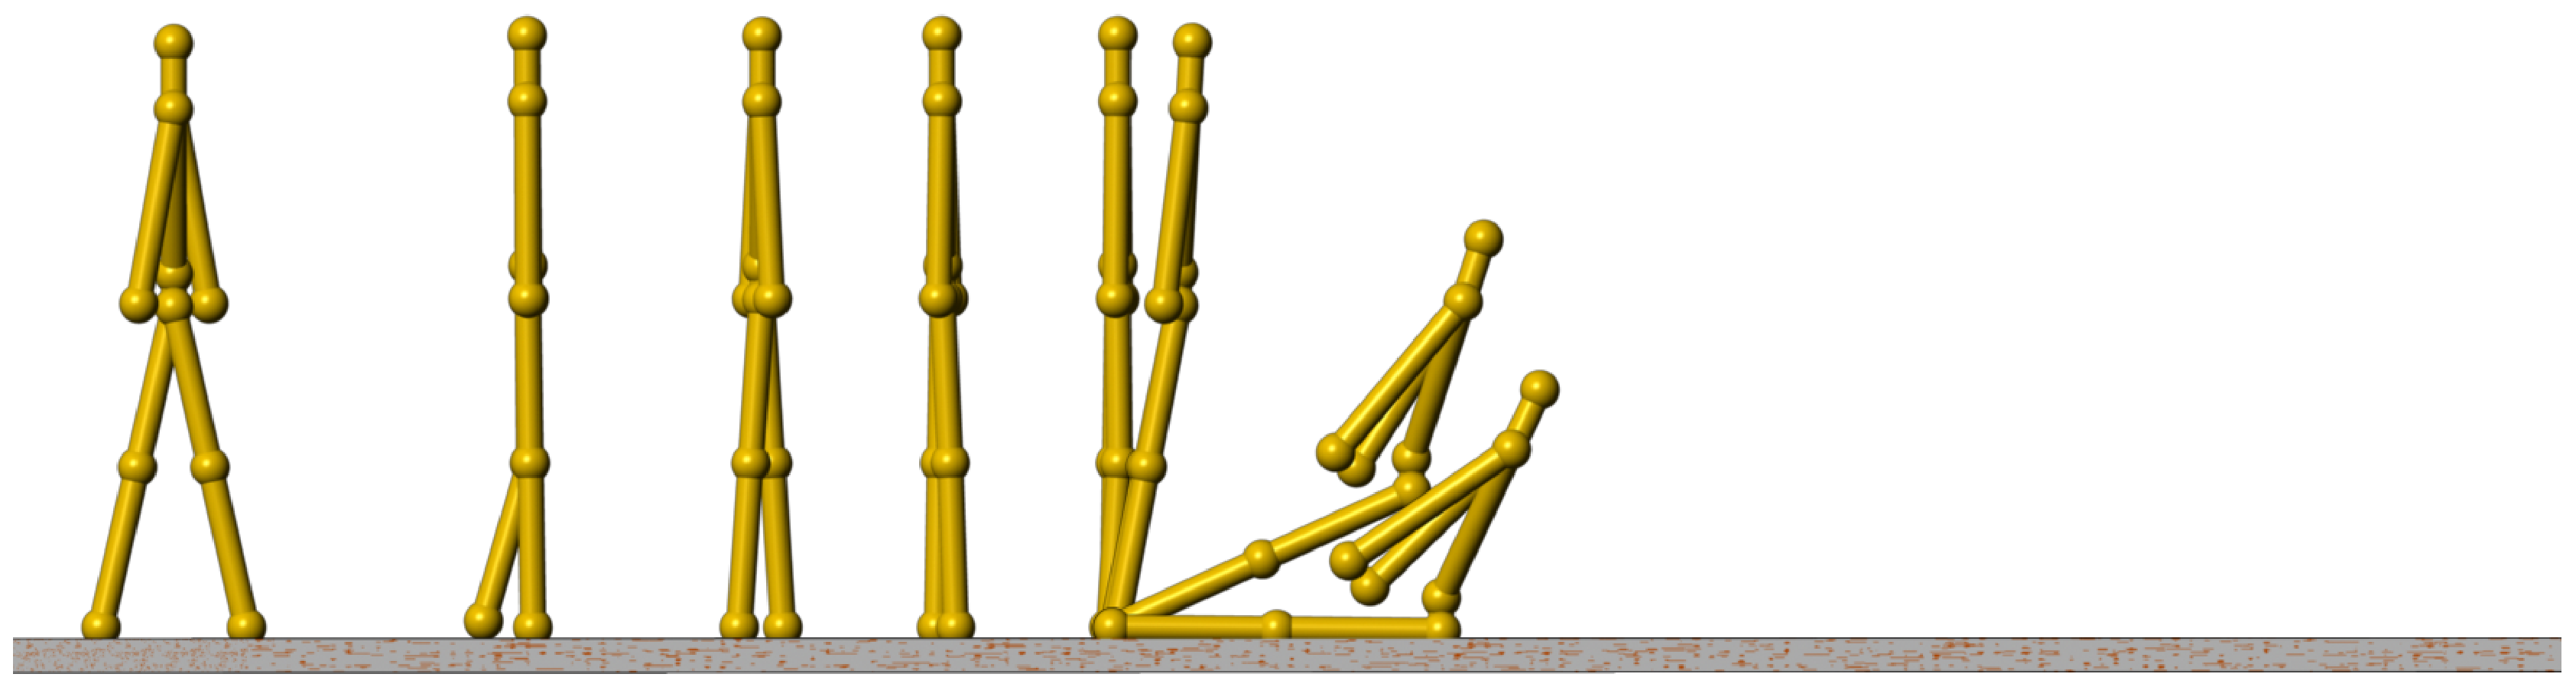
\includegraphics[height=6in]{PlaceHolder}
    \else
      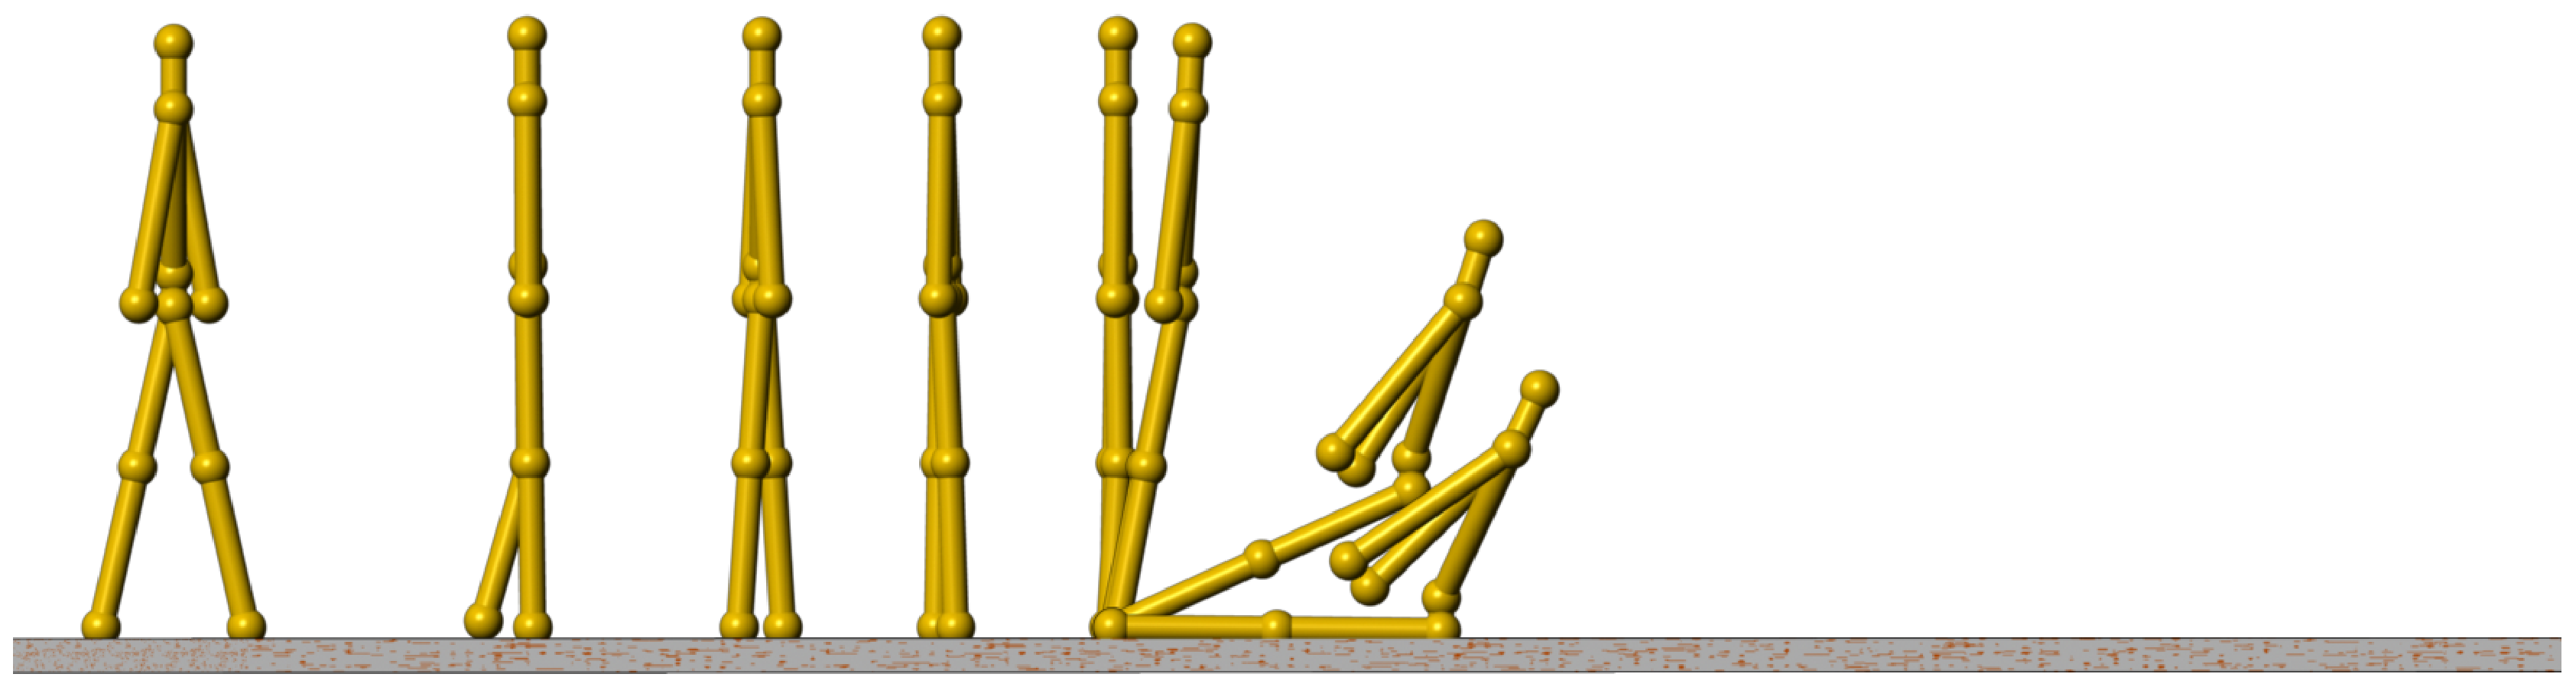
\includegraphics[width=0.7\textwidth]{PlaceHolder}
    \fi
    \caption{Place Holder}
    \label{fig:walkstancestraight}
\end{center}
\end{figure}

\begin{figure}[!htbp]
  \begin{center}
    \leavevmode
    \ifpdf
      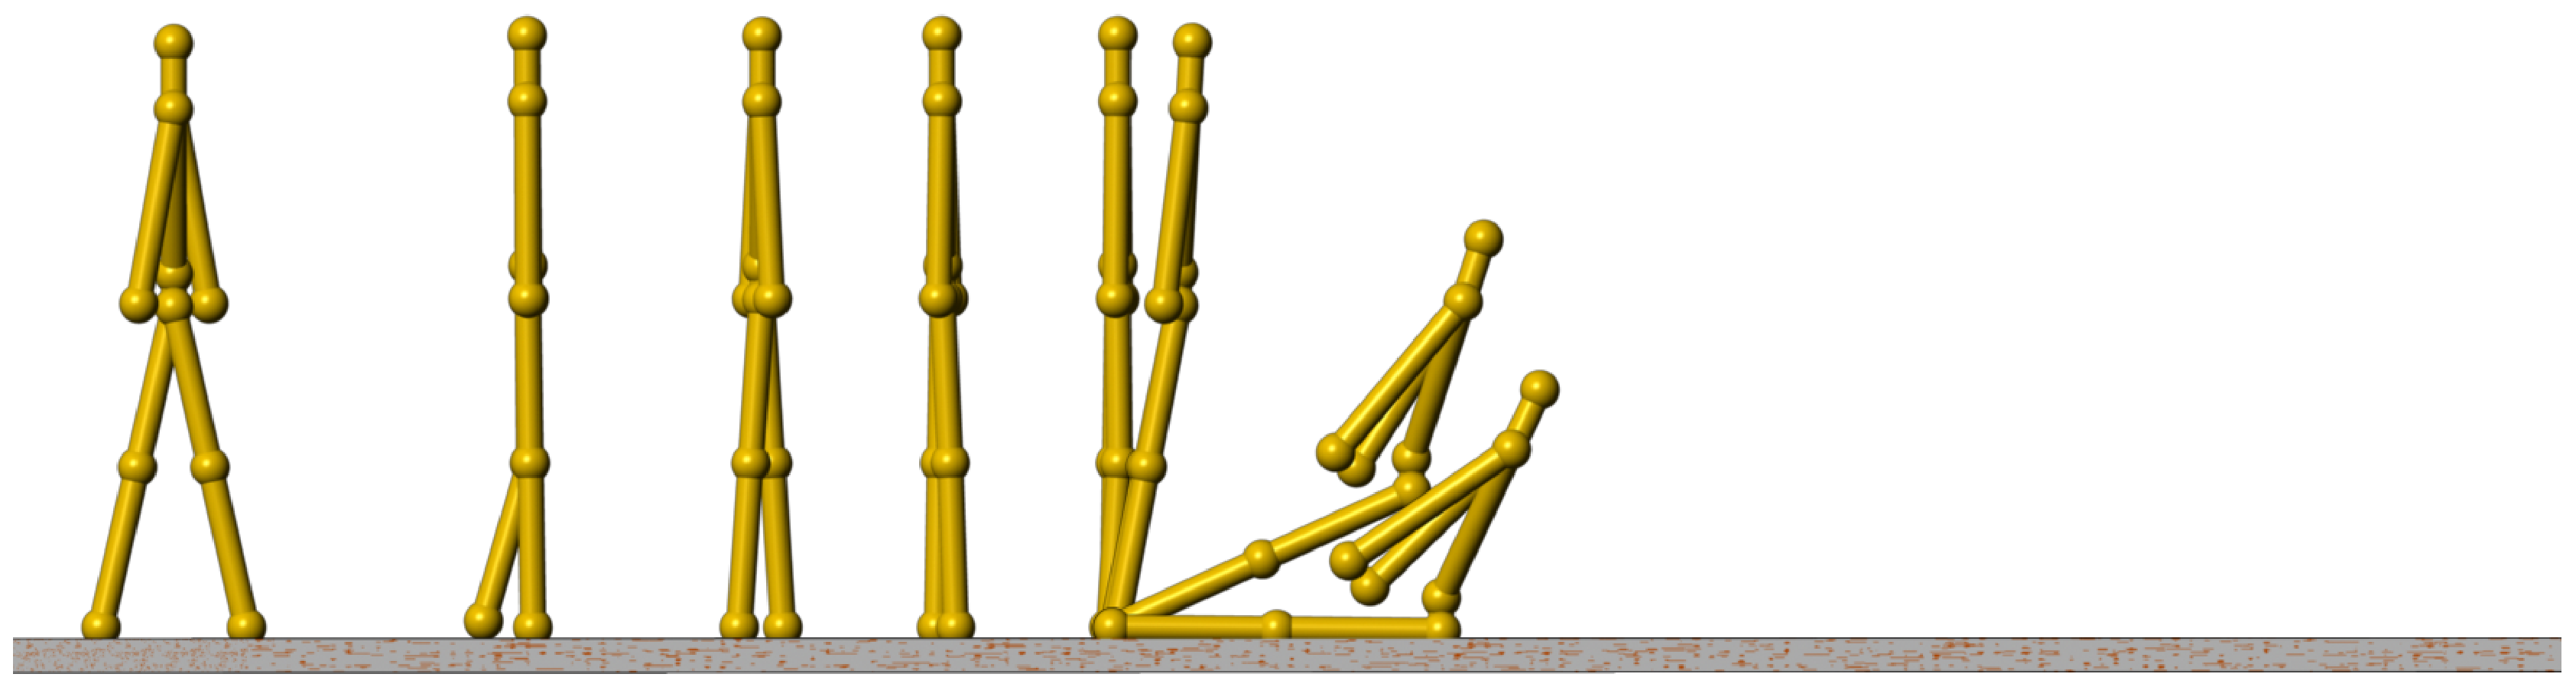
\includegraphics[height=6in]{PlaceHolder}
    \else
      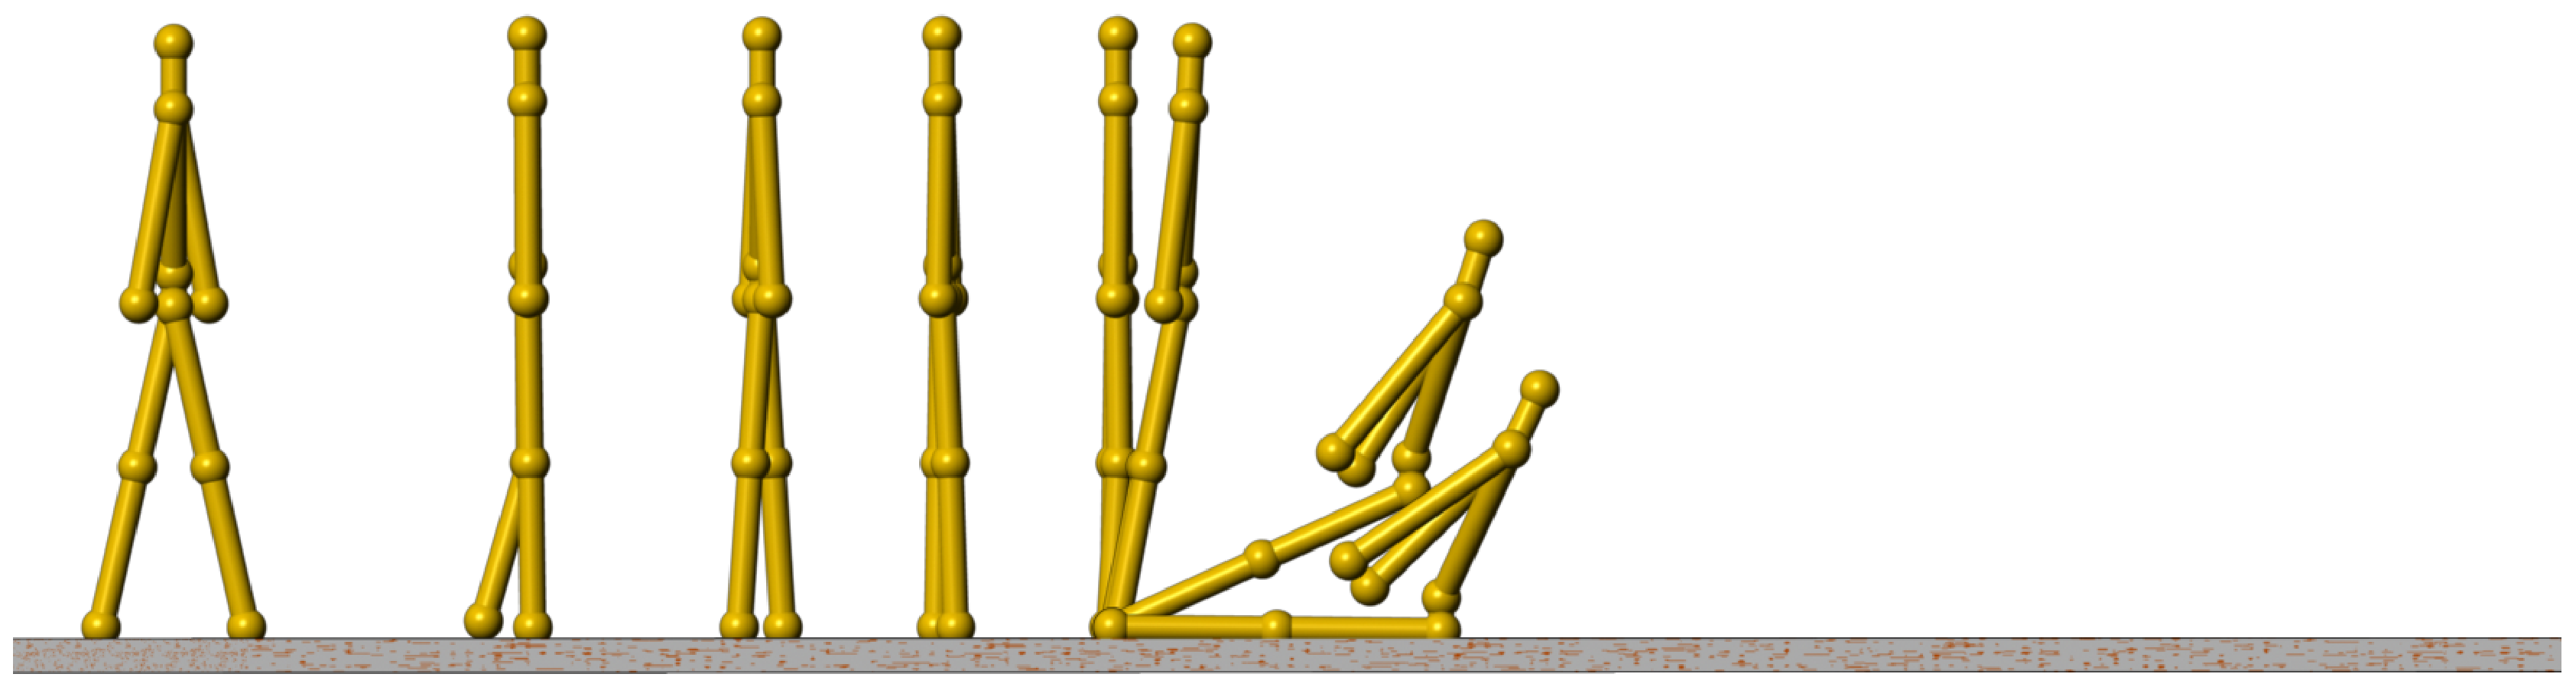
\includegraphics[width=0.7\textwidth]{PlaceHolder}
    \fi
    \caption{Place Holder}
    \label{fig:walkstancebend}
\end{center}
\end{figure}

\subsection{Stance to Walk}
From stance to walk, we must start be making the current state close to the limit circle of walking.
we should place the state of the near the position of start swing position (show in blue).
On the limit circle of stancing, this is the position that the leg is moving forward at maxim speed and the positon of the hip is in the middle between the two legs.
if we switch to the walker at this time, then it will begin to walk.



from walking to stance, there the height has to be increase, so there is only one scheme for straight the knees.
the scheme we use is to keep the supporting leg straight then the make the swing leg from bend to straight.

as show in figure
\begin{figure}[!htbp]
  \begin{center}
    \leavevmode
    \ifpdf
      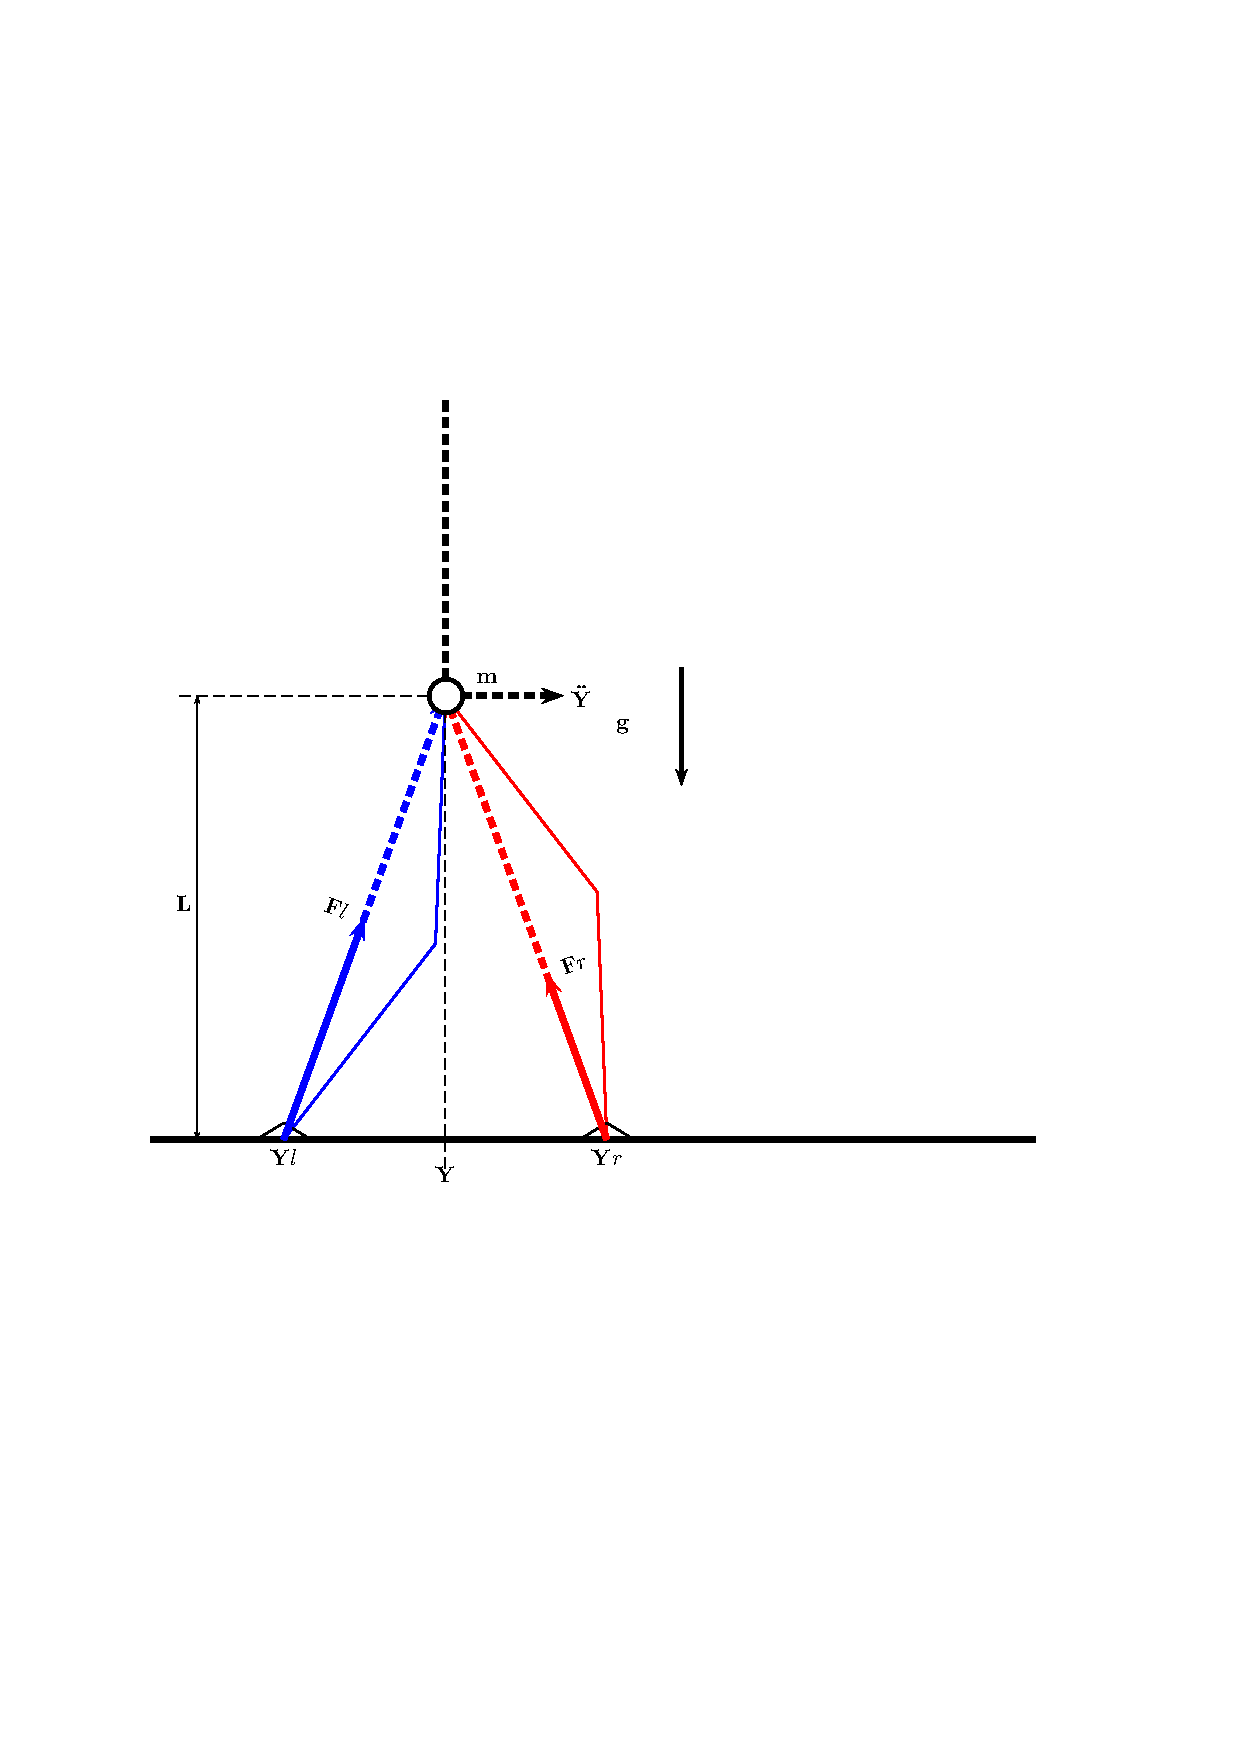
\includegraphics[height=6in]{stancefigure}
    \else
      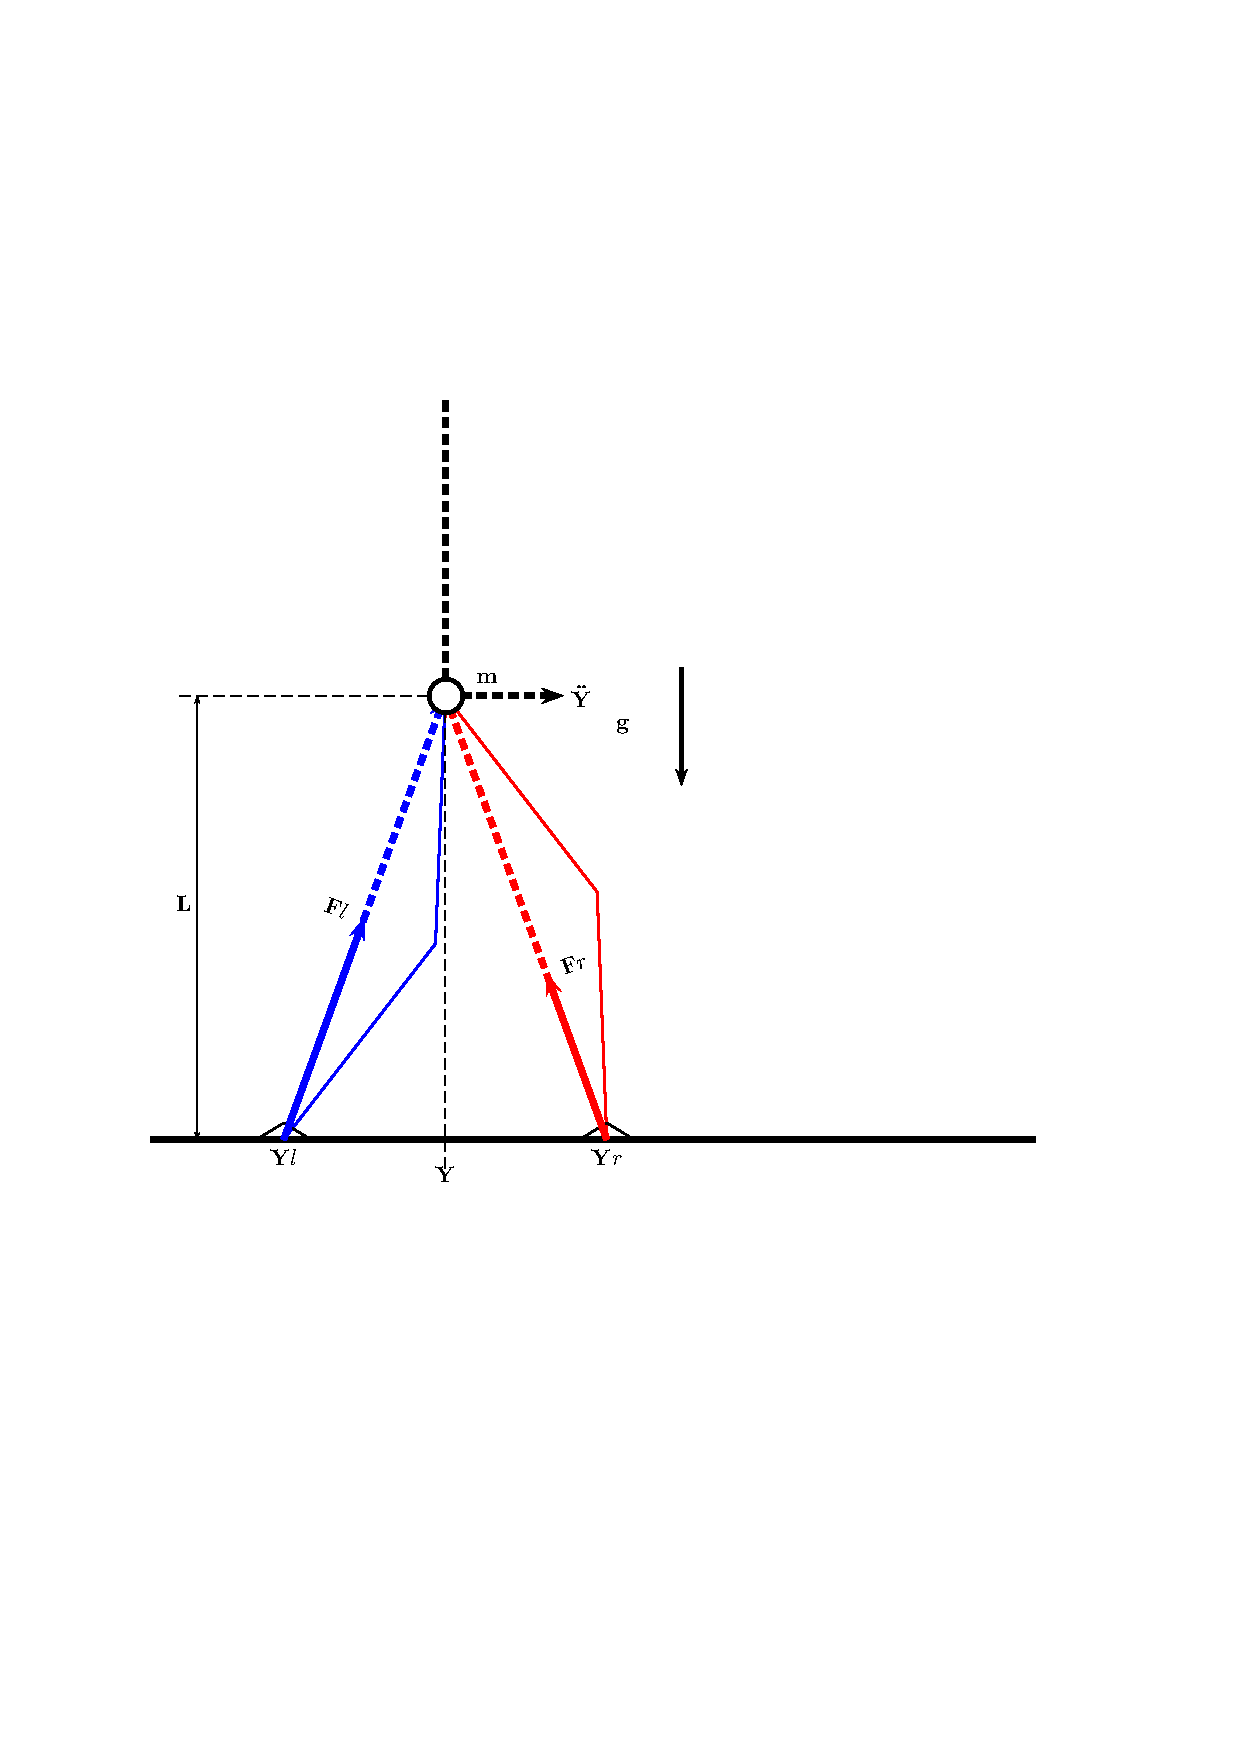
\includegraphics[width=0.7\textwidth]{stancefigure}
    \fi
    \caption{The Place Holder}
    \label{fig:stance2walk}
\end{center}
\end{figure}


A notrivial problem is when switch from stance to walk, 
we can't make two legs both on the limit circle.
Our approach is put the stancing leg on the limit circle, for the stancing leg is more important for maintaining stability.


in the figure above, the stance leg is bit offset of the limit circle, if we put the original swing leg on the limit circl,for it is going to be the support leg in the following walkstep.


\subsection{Speed Action Connection}
When transit from walk to stance, the basin of attraction must include the heelstrike state.
original basin of attraction will not include the heelstrike, a speed action is needed to enlarge the basin of attraction,
There is an alternative to this, we can lower the walker speed, in this way, we lower the effort of balance cotnrol.

Also, if transition from stance to walk, if little effort is executed,the it will start at pos far from the limit cycle.
then to maintain the stability walking, speed action needed to included for start walking slowing.

So the the speedaction of stancing and walking must meet some relationship as
\[
S_sS_w=c
\]

The pheonemon is common for our daily experience, here we give it a methematical meaning.























\subsection{Hyper Dof and Boid System}

Boid like system
some animals like snake and fish have a very flexible verberate. 
And such system are refered to as hyper dof system.
For such kind of system, motion control seems more difficult.

Based on the idea of symmetry and limit circle, we proprose an ad-hoc based idea.
That every joint or every agent are controlled independently,

unlike tradition boid idea,
our research is based on rule based,
 we propose that all the agent are cotnrolled by the same neural ocillator and the same parameters.

The limit cricle will garanty that the final motion will converge to the same one,
so the all the agent will move in an unifield manner.
The different between agent is an phase shift.
That is although all the agent are controlled by the same limit circle, but there is a phase offset between them.
\begin{figure}[ht]
  \centering
  \includegraphics[width=3in]{images/phaseShift.eps}
  \caption{Fish SWimming}
\end{figure}


We apply this method modeling the motion of a long tail fish.
And use the basic mass spring model to model the fish movement.
The advantage of such system over orignal mass spring system is 
Unlike the origianl mass spring system, the speed and size of the vibration can be cotnrolled,
also, numberic error is not a big problem.
So the new system is controllable and also stable.

Figure down shows an mass spring system controlled with cpg.
\begin{figure}[ht]
  \centering
  \includegraphics[width=2.5in]{images/swim.eps}
  \caption{Fish SWimming}
\end{figure}

\section{futurework}
Further Work and Discussion
Motion Synthesis greatly reduced the computational load and generate adaptative motion.
But since it is new and not sophisticated.
Further research is needed.
\subsection{ Modeling More Behaviour}
This method is applicable for lots of system.
But this method greatly relies on the dynamic properties of body environment.
The method is not sensitive for small error, so, local modelling error maybe accepts, but the qualitative property must kept.
This is not a trivial task.
 Some of the key features especially the qualitative dynamic property we are just begin to known.
Further application, fluid dynamic of fish and squid swimming.
\subsection{ More Complex Systems and More Type of Symmetry}
For develop lagrange, symbolic expression need to be provide, for high degree system, this may becomes problematic.
Local frame based Method
\subsection{Data Driven}
Can we find symmetry info from data rather than symbolic differential equation?
\subsection{Symmetry and Boid System}
can symmetry be applied to boid system?





\section*{Acknowledgements}

To Robert, for all the bagels.

\bibliographystyle{acmsiggraph}
\bibliography{AMSI}
\end{document}
